
		\documentclass[a4paper]{article}
		
		%package include
		\usepackage[margin=3cm]{geometry}
		\usepackage[italian]{babel}
		\usepackage[utf8]{inputenc}
		\usepackage[T1]{fontenc}
		\usepackage{graphicx}
		\usepackage{fancyhdr}
		\usepackage{lastpage}
		\usepackage{longtable}
		\usepackage{tabu}
		\usepackage{hyperref}
		\usepackage[hypcap]{caption}
		\usepackage{color}
		\usepackage{xcolor}
		\usepackage{eurosym}
		\usepackage{abstract}
		\usepackage{float}
		\usepackage{listings, lstautogobble}
		\usepackage{amsmath}
		\usepackage{subfigure}
		\usepackage{pifont}
		\usepackage{multirow}

		\colorlet{punct}{red!60!black}
		\definecolor{background}{HTML}{EEEEEE}
		\definecolor{delim}{RGB}{20,105,176}
		\colorlet{numb}{magenta!60!black}


		% per allineare il codice a sinistra invece che al centro
		\lstset{
			autogobble=true,
			escapeinside={(*}{*)}
		}

		\lstdefinelanguage{json}{
		    basicstyle=\normalfont\ttfamily,
		    numbers=left,
		    numberstyle=\scriptsize,
		    stepnumber=1,
		    numbersep=8pt,
		    showstringspaces=false,
		    breaklines=true,
		    frame=lines,
		    backgroundcolor=\color{background},
		    literate=
		     *{0}{{{\color{numb}0}}}{1}
		      {1}{{{\color{numb}1}}}{1}
		      {2}{{{\color{numb}2}}}{1}
		      {3}{{{\color{numb}3}}}{1}
		      {4}{{{\color{numb}4}}}{1}
		      {5}{{{\color{numb}5}}}{1}
		      {6}{{{\color{numb}6}}}{1}
		      {7}{{{\color{numb}7}}}{1}
		      {8}{{{\color{numb}8}}}{1}
		      {9}{{{\color{numb}9}}}{1}
		      {:}{{{\color{punct}{:}}}}{1}
		      {,}{{{\color{punct}{,}}}}{1}
		      {\{}{{{\color{delim}{\{}}}}{1}
		      {\}}{{{\color{delim}{\}}}}}{1}
		      {[}{{{\color{delim}{[}}}}{1}
		      {]}{{{\color{delim}{]}}}}{1},
		}
		

		%macro definitions
		\newcommand{\groupname}{Kaizen Team}
\newcommand{\projectname}{Norris}

\newcommand{\proponente}{Maccagnan Alessandro}
\newcommand{\committente}{Vardanega Tullio}

\newcommand{\insglo}[1]{#1{\ped G}}
\newcommand{\ignoreglo}[1]{#1}
\newcommand{\insdate}[3]{#3-#2-#1}
\newcommand{\instime}[2]{#1-#2}
\newcommand{\insuri}[1]{\textcolor{blue}{\texttt{\url{#1}}}}
\newcommand{\inspath}[1]{\texttt{#1}}
\newcommand{\insrole}[1]{\textit{#1}}
\newcommand{\insdoc}[1]{\textit{“#1”}}
\newcommand{\insfile}[1]{“\texttt{#1}”}
\newcommand{\insrev}[1]{\textbf{#1}}
\newcommand{\insphase}[1]{\textbf{#1}}

		\newcommand{\doctitle}{Specifica Tecnica}
		\newcommand{\lastversion}{5.00}
		

		%abstract font
		\renewcommand{\abstractnamefont}{\huge\bfseries}
		\renewcommand{\abstracttextfont}{\large}

		%hyperred
		\hypersetup{
			linktoc=all,
			colorlinks=true,
			allcolors=black,
			urlcolor=blue,
			bookmarksdepth=100
		}

		%section counters
		\makeatletter
		\newcommand\level[1]{%
			\ifcase#1\relax\expandafter\chapter\or
				\expandafter\section\or
				\expandafter\subsection\or
				\expandafter\subsubsection\else
				\def\next{\@level{#1}}\expandafter\next
			\fi}
		\newcommand{\@level}[1]{%
			\@startsection{level#1}%
				{#1}%
				{\z@}%
				{-3.25ex\@plus -1ex \@minus -.2ex}%
				{1.5ex \@plus .2ex}%
				{\normalfont\normalsize\bfseries}}

		\newdimen\@numsdim
		\newdimen\@dotsdim
		{\normalfont\normalsize
			\sbox\z@{0}\global\@numsdim=\wd\z@
			\sbox\z@{.}\global\@dotsdim=\wd\z@
		}

		\newdimen\@numindent
		\newdimen\@textindent
		\setlength{\@numindent}{15pt}
		\setlength{\@textindent}{15pt}


		\newcounter{level4}[subsubsection]
		\@namedef{thelevel4}{\thesubsubsection.\arabic{level4}}
		\@namedef{level4mark}#1{}
		%\def\l@section{\@dottedtocline{1}{\dimexpr\@numindent*0\relax}{\dimexpr\@dotsdim*0+\@numsdim*1+\@textindent\relax}}
		\def\l@subsection{\@dottedtocline{2}{\dimexpr\@numindent*1\relax}{\dimexpr\@dotsdim*1+\@numsdim*2+\@textindent\relax}}
		\def\l@subsubsection{\@dottedtocline{3}{\dimexpr\@numindent*2\relax}{\dimexpr\@dotsdim*2+\@numsdim*3+\@textindent\relax}}
		\@namedef{l@level4}{\@dottedtocline{4}{\dimexpr\@numindent*3\relax}{\dimexpr\@dotsdim*3+\@numsdim*4+\@textindent\relax}}

		\count@=4
		\def\@ncp#1{\number\numexpr\count@+#1\relax}
		\loop\ifnum\count@<100
			\begingroup\edef\x{\endgroup
				\noexpand\newcounter{level\@ncp{1}}[level\number\count@]
				\noexpand\@namedef{thelevel\@ncp{1}}{%
					\noexpand\@nameuse{thelevel\@ncp{0}}.\noexpand\arabic{level\@ncp{1}}}
				\noexpand\@namedef{level\@ncp{1}mark}####1{}%
				\noexpand\@namedef{l@level\@ncp{1}}%
					{\noexpand\@dottedtocline%
						{\@ncp{1}}%
						{\dimexpr\@numindent*\@ncp{0}\relax}%
						{\the\dimexpr\@dotsdim*\@ncp{0}+\@numsdim*\@ncp{1}+\@textindent\relax}}}%
			\x
			\expandafter\edef\csname toclevel@level\the\count@\endcsname{\the\count@}%
			\advance\count@\@ne
		\repeat
		\makeatother
		
		\setcounter{tocdepth}{100}
		\setcounter{secnumdepth}{100}

		

		%fancyhdr config
		\fancyhf{}
		\fancyhead[L]{
\includegraphics[scale=0.05]{Pics/Logo} 
\includegraphics[height=7mm]{Pics/KaizenTeam}}
		\fancyhead[R]{\Large \bfseries \doctitle \vspace{0.1mm}}

		\fancypagestyle{roman}{
			\hypersetup{linkcolor=black}
			\pagenumbering{Roman}
			\fancyfoot[C]{\thepage{}}
		}

		\fancypagestyle{plain}{
			\hypersetup{linkcolor=blue}
			\pagenumbering{arabic}
			\fancyfoot[C]{\thepage{} di \pageref*{LastPage}}
		}

		
		%space between paragraph
		\raggedbottom
		


		\begin{document}

			\pagestyle{roman}
			\begin{titlepage}
  \begin{center}
	
	
\includegraphics{Pics/KaizenTeam} \\ [1cm]
	
	
\includegraphics[scale=0.6]{Pics/Logo} \\ [1cm]

	
\includegraphics[scale=0.3]{Pics/Norris} \\ [0.5cm]
	
\includegraphics[scale=1]{Pics/CoffeeStrap} \\ [2cm]

	
	\hrule
	\vspace{3mm}
	\Huge{\textbf{\doctitle{} v\lastversion{}}}
	\vspace{3mm}
	\hrule


	\vspace{2cm}

	\begin{minipage}{0.49\textwidth}
		\raggedright \large info@kaizenteam.it
	\end{minipage}
	\begin{minipage}{0.49\textwidth}
		\raggedleft \large \insuri{http://www.kaizenteam.it/}
	\end{minipage}

  \end{center}
\end{titlepage}

			\newpage
			

				\begin{center}
					\tabulinesep=6pt
					\begin{tabu} {X[r]|X[l]}
						\textbf{Versione} & 5.00 \\
						\textbf{Data redazione} & 2015-06-13 \\
						\textbf{Redazione} & \parbox[t]{0.4\textwidth}{Pavanello Fabio Matteo} \\
						\textbf{Verifica} & \parbox[t]{0.4\textwidth}{ Moretto Alessandro \\ Bigarella Chiara} \\
						\textbf{Approvazione} & \parbox[t]{0.4\textwidth}{Carlon Chiara} \\
						\textbf{Uso} & Esterno \\
						\textbf{Distribuzione} & \parbox[t]{0.4\textwidth}{\groupname{} \\ Prof. Vardanega Tullio \\ Prof. Cardin Riccardo \\ CoffeeStrap} \\
					\end{tabu}
				\end{center}

	
			\newpage
			
			\section*{Diario delle modifiche}
				\addtocounter{table}{-1}
				\tabulinesep=3pt
				\begin{longtabu} to \textwidth {|X[c,m]|X[c,m]|X[c,m]|X[c,m]|X[c,m]|}
					\hline
					\rowfont{\bf}
					Versione &
					Data &
					Autore &
					Ruolo &
					Descrizione \\
					\hline
					\endhead
					5.00 &
						2015-06-13 &
						Carlon Chiara &
						Project Manager &
						Approvazione del documento \\
						\hline
					4.04 &
						2015-06-12 &
						Bigarella Chiara &
						Verificatore &
						Verifica incrementi \\
						\hline
					4.03 &
						2015-06-12 &
						Pavanello Fabio Matteo &
						Progettista &
						Fornito maggior dettaglio sulle relazioni individuate tra le componenti \\
						\hline
					4.02 &
						2015-06-11 &
						Moretto Alessandro &
						Verificatore &
						Verifica incrementi \\
						\hline
					4.01 &
						2015-06-10 &
						Pavanello Fabio Matteo &
						Progettista &
						Correzione errori segnalati in RQ \\
						\hline
					4.00 &
						2015-05-27 &
						Pavanello Fabio Matteo &
						Project Manager &
						Approvazione del documento \\
						\hline
					3.16 &
						2015-03-29 &
						Rubin Marco &
						Verificatore &
						Verifica incrementi \\
						\hline
					3.15 &
						2015-05-10 &
						Davide Dal Bianco &
						Verificatore &
						Verifica incrementi \\
						\hline
					3.14 &
						2015-05-10 &
						Bigarella Chiara &
						Progettista &
						Aggiunto paragrafo per spiegare l'utilizzo delle classi factory \\
						\hline
					3.13 &
						2015-05-10 &
						Moretto Alessandro &
						Verificatore &
						Verifica incrementi architettura di Norris e Chuck \\
						\hline
					3.12 &
						2015-05-10 &
						Bucco Riccardo &
						Progettista &
						Lieve modifica architettura Norris e Chuck \\
						\hline
					3.11 &
						2015-05-09 &
						Bucco Riccardo &
						Progettista &
						Spostamento pattern dopo la definizione dell'architettura \\
						\hline
					3.10 &
						2015-05-09 &
						Moretto Alessandro &
						Verificatore &
						Verifica incrementi architettura \\
						\hline
					3.09 &
						2015-05-08 &
						Bigarella Chiara &
						Progettista &
						Correzioni errori rilevati dalla verifica dell'architettura dell'applicazione android \\
						\hline
					3.08 &
						2015-05-08 &
						Moretto Alessandro &
						Verificatore &
						Verifica architettura \\
						\hline
					3.07 &
						2015-05-08 &
						Bigarella Chiara &
						Progettista &
						Modifica architettura dell'applicazione android, da MVC a MVP \\
						\hline
					3.06 &
						2015-05-08 &
						Pavanello Fabio Matteo &
						Verificatore &
						Verifica incrementi \\
						\hline
					3.05 &
						2015-05-08 &
						Carlon Chiara &
						Progettista &
						Approfondita descrizione pattern Bridge \\
						\hline
					3.04 &
						2015-05-08 &
						Bigarella Chiara &
						Progettista &
						Correzione piccoli errori segnalati in RP \\
						\hline
					3.03 &
						2015-05-07 &
						Dal Bianco Davide &
						Verificatore &
						Verifica incrementi \\
						\hline
					3.02 &
						2015-05-07 &
						Carlon Chiara &
						Amministratore &
						Aggiunti svantaggi tecnologie \\
						\hline
					3.01 &
						2015-05-07 &
						Bucco Riccardo &
						Progettista &
						Modificati riferimenti informativi \\
						\hline
					3.00 &
						2015-05-03 &
						Bigarella Chiara &
						Project Manager &
						Approvazione del documento \\
						\hline
					2.02 &
						2015-04-24 &
						Bucco Riccardo &
						Verificatore &
						Verifica modifiche Chuck \\
						\hline
					2.01 &
						2015-04-04 &
						Rubin Marco &
						Progettista &
						Apporto di piccole modifiche architettura Chuck \\
						\hline
					2.00 &
						2015-04-20 &
						Dal Bianco Davide &
						Project Manager &
						Approvazione del documento \\
						\hline
					1.02 &
						2015-04-06 &
						Moretto Alessandro &
						Verificatore &
						Verifica incremento \\
						\hline
					1.01 &
						2015-04-04 &
						Rubin Marco &
						Progettista &
						Apporto di piccole modifiche architetturale Norris \\
						\hline
					1.00 &
						2015-03-31 &
						Rubin Marco &
						Project Manager &
						Approvazione del documento \\
						\hline
					0.16 &
						2015-03-31 &
						Pavanello Fabio Matteo &
						Verificatore &
						Verifica documento \\
						\hline
					0.15 &
						2015-03-29 &
						Bucco Riccardo &
						Progettista &
						Stesura ed importazione tracciamento \\
						\hline
					0.14 &
						2015-03-29 &
						Dal Bianco Davide &
						Project Manager &
						Stesura stime di fattibilità e di bisogno di risorse \\
						\hline
					0.13 &
						2015-03-27 &
						Carlon Chiara &
						Verificatore &
						Verifica componenti applicazione Android \\
						\hline
					0.12 &
						2015-03-26 &
						Pavanello Fabio Matteo &
						Verificatore &
						Verifica componenti Chuck \\
						\hline
					0.11 &
						2015-03-26 &
						Carlon Chiara &
						Verificatore &
						Verifica sezione Dashboard \\
						\hline
					0.10 &
						2015-03-26 &
						Bucco Riccardo &
						Progettista &
						Stesura sezione mockup Dashboard \\
						\hline
					0.09 &
						2015-03-26 &
						Carlon Chiara &
						Verificatore &
						Verifica componenti Norris \\
						\hline
					0.08 &
						2015-03-24 &
						Moretto Alessandro &
						Progettista &
						Stesura e descrizione componenti applicazione Android \\
						\hline
					0.07 &
						2015-03-24 &
						Bucco Riccardo &
						Progettista &
						Stesura e descrizione componenti Chuck \\
						\hline
					0.06 &
						2015-03-23 &
						Dal Bianco Davide &
						Progettista &
						Stesura e descrizione componenti Norris \\
						\hline
					0.05 &
						2015-03-15 &
						Pavanello Fabio Matteo &
						Verificatore &
						Verifica architettura \\
						\hline
					0.04 &
						2015-03-12 &
						Bigarella Chiara &
						Progettista &
						Stesura architettura generale \\
						\hline
					0.03 &
						2015-03-07 &
						Carlon Chiara &
						Verificatore &
						Verifica documento \\
						\hline
					0.02 &
						2015-03-06 &
						Moretto Alessandro &
						Progettista &
						Stesura tecnologie utilizzate \\
						\hline
					0.01 &
						2015-03-05 &
						Bigarella Chiara &
						Progettista &
						Struttura ed introduzione del documento \\
						\hline
					
				\end{longtabu}

	
			\newpage

			
			\tableofcontents
			\newpage
			\listoftables
			\newpage
			\listoffigures
			\newpage
			\pagestyle{plain}

			
		\newpage
		% !TEX encoding = UTF-8 Unicode
\section{Introduzione}
	\subsection{Scopo del documento}
		Tale documento ha lo scopo di pianificare il modo e i tempi in cui verranno svolte le attività dai membri del gruppo \groupname{}. \\In particolare, gli scopi di tale documento sono:
		\begin{itemize}
			\item descrivere il ciclo di vita scelto per il prodotto;
			\item fissare le varie fasi di sviluppo esplicandone scopo e dettagli;
			\item analizzare a gestire gli eventuali rischi;
			\item descrivere cosa dovrà esser fatto nelle varie fasi di sviluppo;
			\item preventivare l'impegno delle risorse;
			\item calcolare il consuntivo di utilizzo delle risorse durante lo svolgimento del progetto.
		\end{itemize}
	\subsection{Riferimenti utili}
		\subsubsection{Glossario}
		Al fine di evitare ogni genere di ambiguità relativa al linguaggio o ai termini utilizzati nei documenti, si allega il documento \insfile{Glossario v1.0}.
		\subsubsection{Normativi}
			\begin{itemize}
				\item\textbf{Capitolato D'Appalto C3}: \projectname{}: Real-time Business Intelligence. Reperibile all'indirizzo: \insuri{http://www.math.unipd.it/~tullio/IS-1/2014/Progetto/C3.pdf}
				\item\textbf{Norme Di Progetto}: "Norme Di Progetto v1.0".
			\end{itemize}
		\subsubsection{Informativi}
			\begin{itemize}
				\item \textbf{Analisi dei Requisiti}: “Analisi Dei Requisiti v1.0”;
				\item \textbf{Piano di Qualifica}: “Piano Di Qualifica v1.0”;
				\item \textbf{Studio di Fattibilità}: “Studio Di Fattibilità v1.0”;
				\item \textbf{Software Engineering - Ian Sommerville - 9th Edition (2010)}: Part 4 - Software Management;
				\item \textbf{Slide dell’insegnamento Ingegneria del Software modulo A}: Il ciclo di vita del software, gestione di progetto.
			\end{itemize}
	
		\newpage
		\level{1}{Tecnologie utilizzate}
In questa sezione sono elencate le principali tecnologie utilizzate per lo sviluppo del progetto. Per ognuna di esse viene descritto lo scopo per il quale vengono usate ed i vantaggi che se ne ricavano.
\level{2}{Node.js}
\level{3}{Descrizione}
L'utilizzo di \insglo{Node.js} è stato richiesto dal proponente. Si tratta di un sistema run-time cross-platform che utilizza l'engine Google V8 \insglo{JavaScript} per eseguire il codice; viene utilizzato nello sviluppo di applicazioni real-time, lato \insglo{server} e di rete. Nel progetto viene usato per la realizzazione della libreria come piattaforma di sviluppo.
\level{3}{Vantaggi}
I vantaggi nell'utilizzo di \insglo{Node.js} sono i seguenti:
\begin{itemize}
\item fornisce una semplice soluzione per lo sviluppo di programmi scalabili;
\item essendo leggero ed efficiente è particolarmente indicato per applicazioni real-time con un intensivo uso di dati;
\item usa un sistema I/O asincrono, non bloccante, basato su eventi; questo permette di sviluppare più facilmente sistemi responsivi.
\end{itemize}
\level{3}{Svantaggi}
Seguono gli svantaggi rilevati nell'utilizzo di \insglo{Node.js}:
\begin{itemize}
	\item essendo un linguaggio di recente creazione, alcuni moduli risultano instabili;
	\item essendo un linguaggio single-threaded, non è performante in caso di applicazioni con uso intensivo di CPU;
	\item utilizzando un sistema I/O asincrono, è possibile che l'uso di \insglo{callback} risulti eccessivo.
\end{itemize}

\level{2}{Socket.io}
\level{3}{Descrizione}
L'uso di \insglo{Socket.io} è stato richiesto dal proponente. È una libreria \insglo{JavaScript} che permette comunicazioni real-time bidirezionali e basate su eventi. Viene utilizzato per implementare la trasmissione degli aggiornamenti dei grafici.
\level{3}{Vantaggi}
L'utilizzo di \insglo{Socket.io} fornisce i seguenti vantaggi:
\begin{itemize}
\item permette di creare comunicazioni bi-direzionali tra \insglo{client} e \insglo{server};
\item gestisce la connessione in modo trasparente;
\item ogniqualvolta il \insglo{browser} lo supporti usa il protocollo \insglo{WebSocket}, il quale fornisce canali di comunicazione bidirezionali simultanei attraverso una singola connessione \insglo{TCP}.
\end{itemize}
\level{3}{Svantaggi}
L'utilizzo di \insglo{Socket.io} porta, anche, ad alcuni svantaggi:
\begin{itemize}
	\item richiede che, sia \insglo{client} che \insglo{server}, utilizzino le librerie di \insglo{Socket.io};
	\item essendo una tecnologia di recente creazione, soffre ancora di alcuni bug.
\end{itemize}

\level{2}{Express.js}
\level{3}{Descrizione}
\insglo{Express.js} è un \insglo{framework} di \insglo{Node.js} che mette a disposizione un \insglo{middleware} utilizzabile per la realizzazione dell'infrastruttura web. Il suo utilizzo è stato richiesto dal proponente.
\level{3}{Vantaggi}
\insglo{Express.js} permette di estendere il modulo \texttt{http} di \insglo{Node.js} rendendo più facile la gestione dell'indirizzamento del \insglo{server}, delle risposte, dei cookie e delle richieste di stato \insglo{HTTP}.
\level{3}{Svantaggi}
Non sono stati rilevati grossi svantaggi nell'uso di \insglo{Express.js}, il quale risulta essere un buon \insglo{framework} che fornisce molti metodi per estendere il modulo \insglo{http} di \insglo{Node.js}.

\level{2}{HTML5}
\level{3}{Descrizione}
Si è scelto di utilizzare HTML5 come \insglo{linguaggio di markup} per la creazione delle pagine web.
\level{3}{Vantaggi}
I vantaggi dell'uso di HTML5 sono i seguenti:
\begin{itemize}
\item è il linguaggio utilizzato dalla libreria \insglo{Chart.js} per produrre i grafici;
\item HTML5 è supportato da tutti i più recenti \insglo{browser};
\item assieme a CSS permette di creare pagine web più interattive;
\item è stato decretato standard dal W3C.
\end{itemize}
\level{3}{Svantaggi}
Nell'uso di HTML5, sono stati rilevati i seguenti svantaggi:
\begin{itemize}
\item è supportato solo dalle versioni più recenti dei \insglo{browser};
\item è un linguaggio ancora in via di sviluppo, il che comporta un possibile cambiamento dei costrutti; tuttavia la maggior parte di questo linguaggio è stata considerata stabile.
\end{itemize}

\level{2}{CSS3}
\level{3}{Descrizione}
È stato scelto di usare CSS3 come linguaggio di formattazione dei documenti HTML. Grazie ad esso è possibile fornire un \insglo{layout} alle pagine web per renderle accessibili ed usabili.
\level{3}{Vantaggi}
I vantaggi dell'uso di CSS3 sono i seguenti:
\begin{itemize}
\item permette il riuso del codice, il che comporta una maggiore velocità di caricamento delle pagine web;
\item consente una manutenzione più semplice e veloce;
\item permette la separazione tra la struttura e la presentazione.
\end{itemize}
\level{3}{Svantaggi}
L'unico svantaggio rilevato dall'uso di CSS3 è dato dal fatto che, essendo un linguaggio ancora in via di sviluppo, è supportato (non appieno) solo dai web \insglo{browser} più recenti.

\level{2}{AngularJS}
\level{3}{Descrizione}
AngularJS è un \insglo{framework} \insglo{MVC} \insglo{JavaScript} che fornisce un metodo ben strutturato per la creazione di siti e applicazioni web. Questo \insglo{framework} è la libreria lato \insglo{client} ideale da usare insieme a \insglo{Node.js}.
\level{3}{Vantaggi}
L'utilizzo di AngularJS fornisce i seguenti vantaggi:
\begin{itemize}
\item fornisce un approccio pulito e strutturato per la creazione delle applicazioni lato \insglo{client};
\item utilizza gli oggetti \insglo{JavaScript};
\item facilita la corretta implementazione del \insglo{pattern} \insglo{MVC};
\item fornisce una semplice e flessibile interfaccia di filtraggio che permette di filtrare i dati nel passaggio da Model a View.
\end{itemize}
\level{3}{Svantaggi}
Uno degli svantaggi rilevato nell'uso di \insglo{Angular.js} è la documentazione povera di esempi d'utilizzo. Tuttavia, questo può essere risolto tramite un'approfondita ricerca nel web. Un altro svantaggio deriva dal fatto che il codice non è valido secondo lo standard del W3C. 

\level{2}{Google chart}
\level{3}{Descrizione}
È stato scelto di usare la libreria \insglo{JavaScript} sviluppata da Google per la creazione di grafici in HTML5.
\level{3}{Vantaggi}
I vantaggi dell'uso di \insglo{Google chart} sono i seguenti:
\begin{itemize}
\item consente un facile inserimento dei grafici all'interno di pagine HTML attraverso l'utilizzo di tag <div>;
\item consente un'ampia personalizzazione delle impostazioni dei grafici;
\ fornisce un'ampia galleria di grafici con cui poter eventualmente estendere il framework;
\item essendo modulare, permette di caricare solo i grafici di cui si ha bisogno.
\end{itemize}
\level{3}{Svantaggi}
Non sono stati riscontrati grossi svantaggi nell'uso di tale libreria, la quale è accompagnata da una documentazione organizzata e ben fornita, anche, di numerosi esempi.

\level{2}{DataTables}
\level{3}{Descrizione}
È stato scelto di usare la libreria \insglo{JavaScript} \insglo{DataTables} per la creazione di tabelle in HTML5. Tale libreria permette la creazione di tabelle dinamiche ed interattive. \insglo{DataTables} fornisce delle \insglo{API} per la manipolazione delle tabelle e per l'accesso ai dati contenuti in esse. 
\level{3}{Vantaggi}
L'utilizzo di \insglo{DataTables} offre i seguenti vantaggi:
\begin{itemize}
\item fornisce numerose opzioni aggiuntive ed estensioni, che rendono ampiamente personalizzabili le tabelle create;
\item fornisce metodi di ordinamento dei dati, che possono essere personalizzati a seconda delle necessità;
\item permette il filtraggio dei dati, basato sui dati o sulle righe;
\item permette la personalizzazione delle opzioni di impaginamento delle tabelle, in modo che siano facili da consultare per l'utente finale.
\end{itemize}
\level{3}{Svantaggi}
Nell'uso di \insglo{DataTables} non sono stati rilevati grossi svantaggi. \insglo{DataTables} offre un'ampia documentazione piena di esempi d'uso. Inoltre, grazie al forum, presente sul sito web ufficiale, si possono ottenere risposte ad eventuali problemi o dubbi che sorgono durante l'utilizzo della libreria.

\level{2}{OpenStreetMap}
\level{3}{Descrizione}
È stato scelto di utilizzare OpenStreetMap, per la visualizzazione di Map Charts, un progetto collaborativo finalizzato alla creazione di dati cartografici, liberi e gratuiti a chiunque. Il progetto è stato lanciato poiché molte delle mappe che normalmente si pensano libere, hanno in realtà restrizioni legali o tecniche. OpenStreetMap mette, inoltre, a disposizione i geodati su cui le mappe si basano, al contrario di moltre altre librerie, come Google Maps \insglo{API}.
\level{3}{Vantaggi}
L'utilizzo di OpenStreetMap offre i seguenti vantaggi:
\begin{itemize}
\item libertà: i dati geografici e le mappe di OpenStreetMap sono rilasciati con licenza creata specificamente per proteggere i \insglo{database}, la quale permette la copia, la modifica e la ridistribuzione delle mappe, inoltre sono completamente gratuite, quindi non occorre pagare per usufruire di funzionalità aggiuntive;
\item affidabilità: le mappe sono prive di errori inseriti volutamente per riconoscere le mappe copiate;
\item copertura mondiale: essendo un progetto collaborativo a livello mondiale, offre mappe molto precise di tutto il mondo;
\item flessibilità: i dati di OpenStreetMap possono essere usati in molte maniere diverse, principalmente per creare mappe ma anche per copiarle, trasferirle e modificarle per qualsiasi scopo.
\end{itemize}
\level{3}{Svantaggi}
Gli unici svantaggi, derivanti dall'uso di OpenStreetMap, sono inerenti alla precisione delle mappe, i cui dati non essendo controllati sistematicamente, possono mancare di precisione ed accuratezza.

\level{2}{MPAndroidChart}
\level{3}{Descrizione}
Si è scelto di utilizzare MPAndroidChart, una libreria per la creazione di chart in \insglo{Android}. Essa viene usata per la creazione di \insglo{bar chart} e \insglo{line chart}, ma ne supporta molti altri come pie chart, radar chart e scatter chart. Tale libreria fornisce anche delle funzioni di scaling (ridimensionamento), dragging (trascinamento), selecting (selezione) e di animazione. La scelta di una libreria per la creazione di chart in \insglo{Android} è ricaduta su MPAndroidChart principalmente per le poche librerie a disposizione, tuttavia sono comunque stati trovati alcuni aspetti positivi.
\level{3}{Vantaggi}
MPAndroidChart fornisce i seguenti benefici:
\begin{itemize}
\item ridimensionamento su entrambi gli assi di un chart, tramite touch-\insglo{gesture}, in modo separato;
\item salvataggio dei chart su SD-Card come immagini;
\item template di impostazioni predefinite;
\item legende create automaticamente ma personalizzabili;
\item grafici ampiamente personalizzabili.
\end{itemize}
\level{3}{Svantaggi}
Non sono stati trovati svantaggi nell'uso di tale libreria. Essa è accompagnata da un'ampia documentazione, che ci ha permesso uno studio più rapido e più semplice grazie ai numerosi esempi forniti.

\level{2}{GoogleMaps Android API v2}
\level{3}{Descrizione}
Si è scelto di utilizzare GoogleMaps \insglo{Android} \insglo{API} v2 per la visualizzazione di mappe. Tale libreria permette di aggiungere mappe basate sui dati di Google Maps, alla propria applicazione. Le \insglo{API} gestiscono automaticamente l'accesso ai \insglo{server} di Google Maps, il download dei dati, la visualizzazione della mappa e le risposte alle \insglo{gesture}. Inoltre è possibile usare tali \insglo{API} per aggiungere markers e per cambiare la view di una particolare area di una mappa.
\level{3}{Vantaggi}
L'utilizzo di GoogleMaps \insglo{Android} \insglo{API} v2 fornisce i seguenti vantaggi:
\begin{itemize}
\item è possibile inserire una mappa in un'\insglo{activity} come un fragment, con un semplice frammento di codice \insglo{XML};
\item fornisce nuove funzionalità come: mappe 3D, satellite, terreno, mappe ibride e transizioni animate
\item offre la possibilità di aggiungere la visualizzazione “StreetView”.
\end{itemize}
\level{3}{Svantaggi}
Non sono stati riscontrati grossi svantaggi nell'uso di tale libreria, la quale è accompagnata da una documentazione ben organizzata. Inoltre, si possono trovare facilmente online, molti esempi e tutorial.

	
		\newpage
		\level{1}{Descrizione generale dei prodotti}
    Riportiamo di seguito una descrizione generale dei prodotti. Per una descrizione più dettagliata delle funzionalità dei prodotti, si rimanda al documento \insdoc{Analisi dei Requisiti v6.00}.

    \level{2}{Norris}
        \insglo{Norris} è un \insglo{framework} per \insglo{Node.js} che permette di raccogliere dati provenienti da sorgenti arbitrarie e visualizzarli come grafici in modo semplice e veloce. In particolare mette a disposizione dei suoi utenti due interfacce:
        \begin{itemize}
            \item le \insglo{API} interne (lato \insglo{server});
            \item le \insglo{API} esterne (lato \insglo{client}).
        \end{itemize}
        
        \level{3}{API interne}
        Tramite le \insglo{API} interne, uno sviluppatore può creare quattro tipologie di grafici: \insglo{bar chart}, \insglo{line chart}, \insglo{map chart} e \insglo{table}. Per ogni grafico può configurare le relative impostazioni e può impostare il metodo di aggiornamento dei dati del grafico stesso. L'aggiornamento dei grafici può essere di tre tipologie, a seconda del tipo di grafico:
        \begin{itemize}
            \item \insglo{in place}, supportato da tutti i tipi di chart;
            \item \insglo{stream}, supportato da \insglo{bar chart}, \insglo{line chart} e \insglo{table};
            \item \insglo{movie}, supportato da \insglo{map chart}.
        \end{itemize}
        
        Lo sviluppatore può, inoltre, scegliere di incapsulare alcuni grafici all'interno di una o più pagine web. Le \insglo{API} interne permettono infatti di aggiungere i grafici creati ad una o più pagine web, le quali verranno create in automatico da \insglo{Norris}. Lo sviluppatore, oltre a poter scegliere quali grafici inserire in queste pagine, può configurare le impostazioni di ciascuna di esse. Tra le impostazioni principali ci sono la scelta del titolo e del template della pagina.\\
        Infine, se lo sviluppatore non vuole rendere pubblici i propri grafici, può definire una funzione login, una funzione isLogged e una funzione di logout. Queste verranno eseguite ogni qualvolta venga richiesto di accedere alle informazioni di un grafico.
       
        \level{3}{API esterne}
            Tramite le \insglo{API} esterne, un utente lato \insglo{client} può effettuare l'autenticazione ad un'istanza di \insglo{Norris} esistente e richiedere al \insglo{server} le informazioni inerenti ai grafici presenti in quell'istanza. In particolare l'utente \insglo{client} può richiedere la lista dei grafici presenti nell'istanza, nonché le informazioni di ogni singolo grafico della lista. Le informazioni verranno fornite in formato \insglo{JSON}.

    \level{2}{Chuck}
        \insglo{Chuck}, acronimo di Chart Universal Creator Kit, è una libreria \insglo{JavaScript} lato \insglo{client} che permette di incapsulare un grafico (creato tramite le \insglo{API} interne di \insglo{Norris}) all'interno di una pagina web diversa da quelle create di default da \insglo{Norris}. In particolare lo sviluppatore lato \insglo{client} deve autenticarsi ad un'istanza di \insglo{Norris}, richiedere un grafico e scegliere il tag HTML in cui inserire il grafico. È possibile, inoltre, modificare alcune impostazioni relative al grafico.
    
    \level{2}{Applicazione Android}
        L'applicazione \insglo{Android} permette di visualizzare i grafici di un'istanza di \insglo{Norris} da uno smartphone \insglo{Android}. Essa permette di scegliere l'istanza di \insglo{Norris} alla quale connettersi tramite autenticazione. Una volta autenticato, l'utente può visualizzare la lista di grafici esistenti e i grafici stessi.
    \level{2}{Dashboard APS}
        La \insglo{dashboard} rappresenta un caso d'uso di \projectname{}. In particolare, essa è un'applicazione web utile alla visualizzazione di informazioni riguardanti le linee degli autobus dell'\insglo{APS} di Padova, con aggiornamento real-time.\\
        Attraverso l'uso di una mappa, l'utente finale potrà vedere gli spostamenti, in tempo reale, dei mezzi di trasporto della rete urbana.\\
    
        
\level{1}{Descrizione delle interazioni che i prodotti hanno tra di loro}
    \level{2}{Norris - Chuck}
        \insglo{Norris} e \insglo{Chuck} interagiscono tramite le \insglo{API} esterne, le quali fungono da interfaccia tra \insglo{server} e \insglo{client}. In particolare si possono avere 3 tipologie di interazione:
        \begin{itemize}
            \item autenticazione: precede l'invio di informazioni inerenti un grafico. \insglo{Chuck} manda a \insglo{Norris} l'indirizzo dell'istanza a cui si vuole connettere, assieme ad username e password. \insglo{Norris} controlla se i dati inviati sono corretti e, in caso affermativo, esegue l'autenticazione. Riportiamo di seguito un diagramma esplicativo:
        	\begin{figure}[H]\centering
        		\includegraphics[width=\textwidth]{SpecificaTecnica/Pics/Chuck/Autenticazione.pdf}
        		\caption{Diagramma di attività dell'autenticazione}
    		\end{figure}
	
            \item richiesta inserimento grafico: \insglo{Chuck} manda a \insglo{Norris} una richiesta di informazioni inerenti al grafico che si vuole inserire nella pagina web. \insglo{Norris} controlla se il \insglo{client} è autenticato. In caso negativo, \insglo{Norris} manda una richiesta di autenticazione al \insglo{client}. In caso affermativo, invece, \insglo{Norris} manda le informazioni relative al grafico richiesto aprendo una comunicazione tramite \insglo{websocket}. Il canale rimane aperto fintanto che il \insglo{client} rimane connesso. Riportiamo di seguito un diagramma esplicativo:
            \begin{figure}[H]\centering
        	\includegraphics[width=\textwidth]{SpecificaTecnica/Pics/Chuck/RichiestaGrafico.pdf}
        	\caption{Diagramma di attività della richiesta di inserimento di un grafico}
    		\end{figure}
            \item aggiornamenti del grafico: quando un grafico viene aggiornato lato \insglo{server}, \insglo{Norris} si preoccupa di mandare l'aggiornamento ai \insglo{client} che hanno quel grafico. La comunicazione dell'aggiornamento avviene tramite un canale \insglo{websocket} appositamente creato al momento della richiesta di inserimento del grafico nella pagina web. Riportiamo di seguito un diagramma esplicativo:
            \begin{figure}[H]\centering
        	\includegraphics[width=\textwidth]{SpecificaTecnica/Pics/Chuck/AggiornamentiGrafico.pdf}
        	\caption{Diagramma di attività dell'aggiornamento di un grafico}
    		\end{figure}
        \end{itemize}
    
    \level{2}{Norris - Applicazione Android}
        \insglo{Norris} e l'applicazione \insglo{Android} interagiscono tramite le \insglo{API} esterne, le quali fungono da interfaccia tra \insglo{server} e \insglo{client}. In particolare si possono avere 4 tipologie di interazione:
        \begin{itemize}
            \item Autenticazione: precede l'invio di informazioni inerenti un grafico. L'applicazione \insglo{Android} manda a \insglo{Norris} l'indirizzo dell'istanza a cui si vuole connettere, assieme ad username e password. \insglo{Norris} controlla se i dati inviati sono corretti e, in caso affermativo, esegue l'autenticazione. Se l'autenticazione non va a buon fine, l'applicazione \insglo{Android} mostra un messaggio d'errore. Riportiamo di seguito un diagramma esplicativo:
        	\begin{figure}[H]\centering
        		\includegraphics[width=\textwidth]{SpecificaTecnica/Pics/Applicazione/Autenticazione.pdf}
        		\caption{Diagramma di attività dell'autenticazione}
    		\end{figure}
            \item Richiesta informazioni della lista di grafici: l'applicazione \insglo{Android} manda a \insglo{Norris} una richiesta di informazioni inerenti alla lista di grafici presenti nell'istanza di \insglo{Norris} alla quale ci si è autenticati. \insglo{Norris} controlla se l'utente è autenticato e, in caso affermativo, manda le informazioni relative alla lista di grafici richiesta tramite una richiesta \insglo{HTTP}. Riportiamo di seguito un diagramma esplicativo:
            \begin{figure}[H]\centering
        	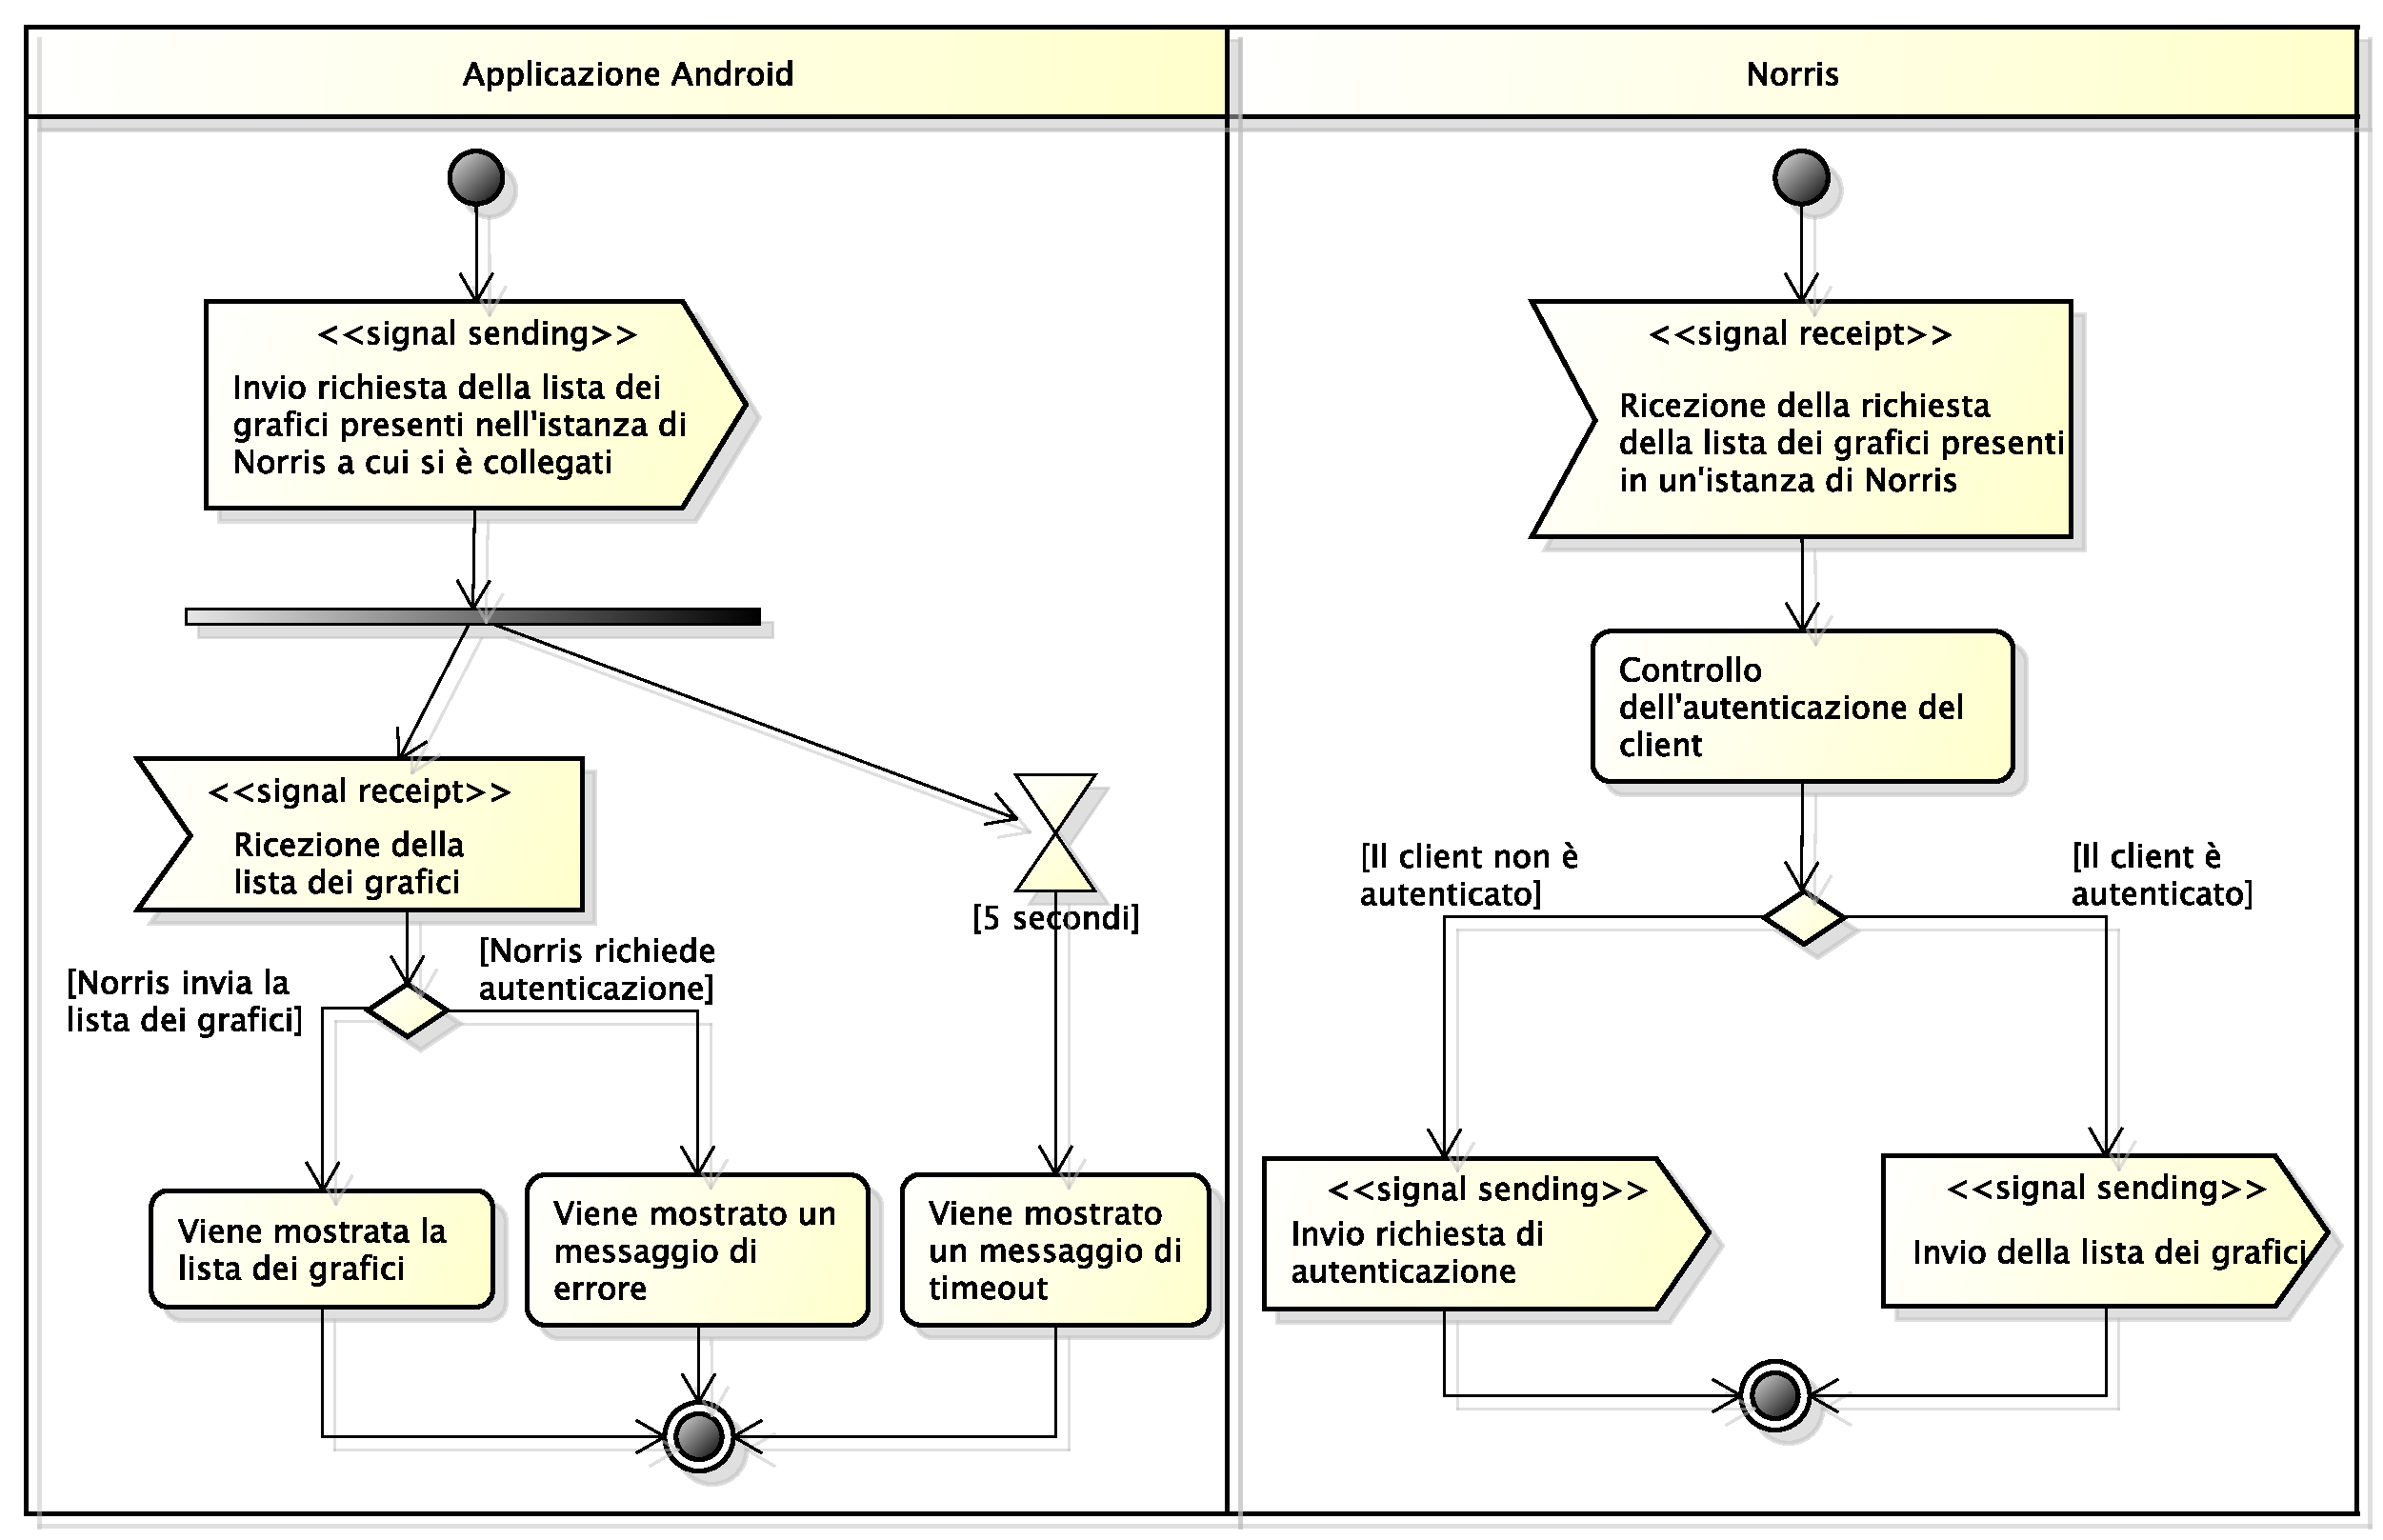
\includegraphics[width=\textwidth]{SpecificaTecnica/Pics/Applicazione/RichiestaLista.pdf}
        	\caption{Diagramma di attività della richiesta delle informazioni di una lista di grafici}
    		\end{figure}
            \item Richiesta informazioni di un grafico: l'applicazione \insglo{Android} manda a \insglo{Norris} una richiesta di informazioni inerenti al grafico che si vuole visualizzare nell'applicazione. \insglo{Norris} controlla se il \insglo{client} è autenticato e, in caso affermativo, manda le informazioni relative al grafico richiesto aprendo una comunicazione tramite \insglo{websocket}. Il canale viene chiuso quando il grafico o l'applicazione sono in background. Riportiamo di seguito un diagramma esplicativo:
            \begin{figure}[H]\centering
        	\includegraphics[width=\textwidth]{SpecificaTecnica/Pics/Applicazione/RichiestaGrafico.pdf}
        	\caption{Diagramma di attività della richiesta delle informazioni di un grafico}
    		\end{figure}
            \item Aggiornamenti del grafico: quando un grafico viene aggiornato lato \insglo{server}, \insglo{Norris} si preoccupa di mandare l'aggiornamento ai \insglo{client} che hanno quel grafico. La comunicazione dell'aggiornamento avviene tramite un canale \insglo{websocket} appositamente creato al momento dell'invio dell'aggiornamento. Il canale viene chiuso quando il grafico o l'applicazione sono in background. Gli aggiornamenti avranno luogo solo quando il grafico è attivo. Se il grafico è in background, gli aggiornamenti vengono ignorati. Riportiamo di seguito un diagramma esplicativo:
            \begin{figure}[H]\centering
        	\includegraphics[width=\textwidth]{SpecificaTecnica/Pics/Applicazione/AggiornamentiGrafico.pdf}
        	\caption{Diagramma di attività dell'aggiornamento di un grafico}
    		\end{figure}
        \end{itemize}

	
		\newpage
		\level{1}{Progettazione architetturale dei prodotti}
	
			\level{4}[DataModel]{Norris::DataModel}
			

		\IfFileExists{DefinizioneDiProdotto/Pics/Classi/Norris--DataModel.pdf}{
			\begin{figure}[H]
				\centering
				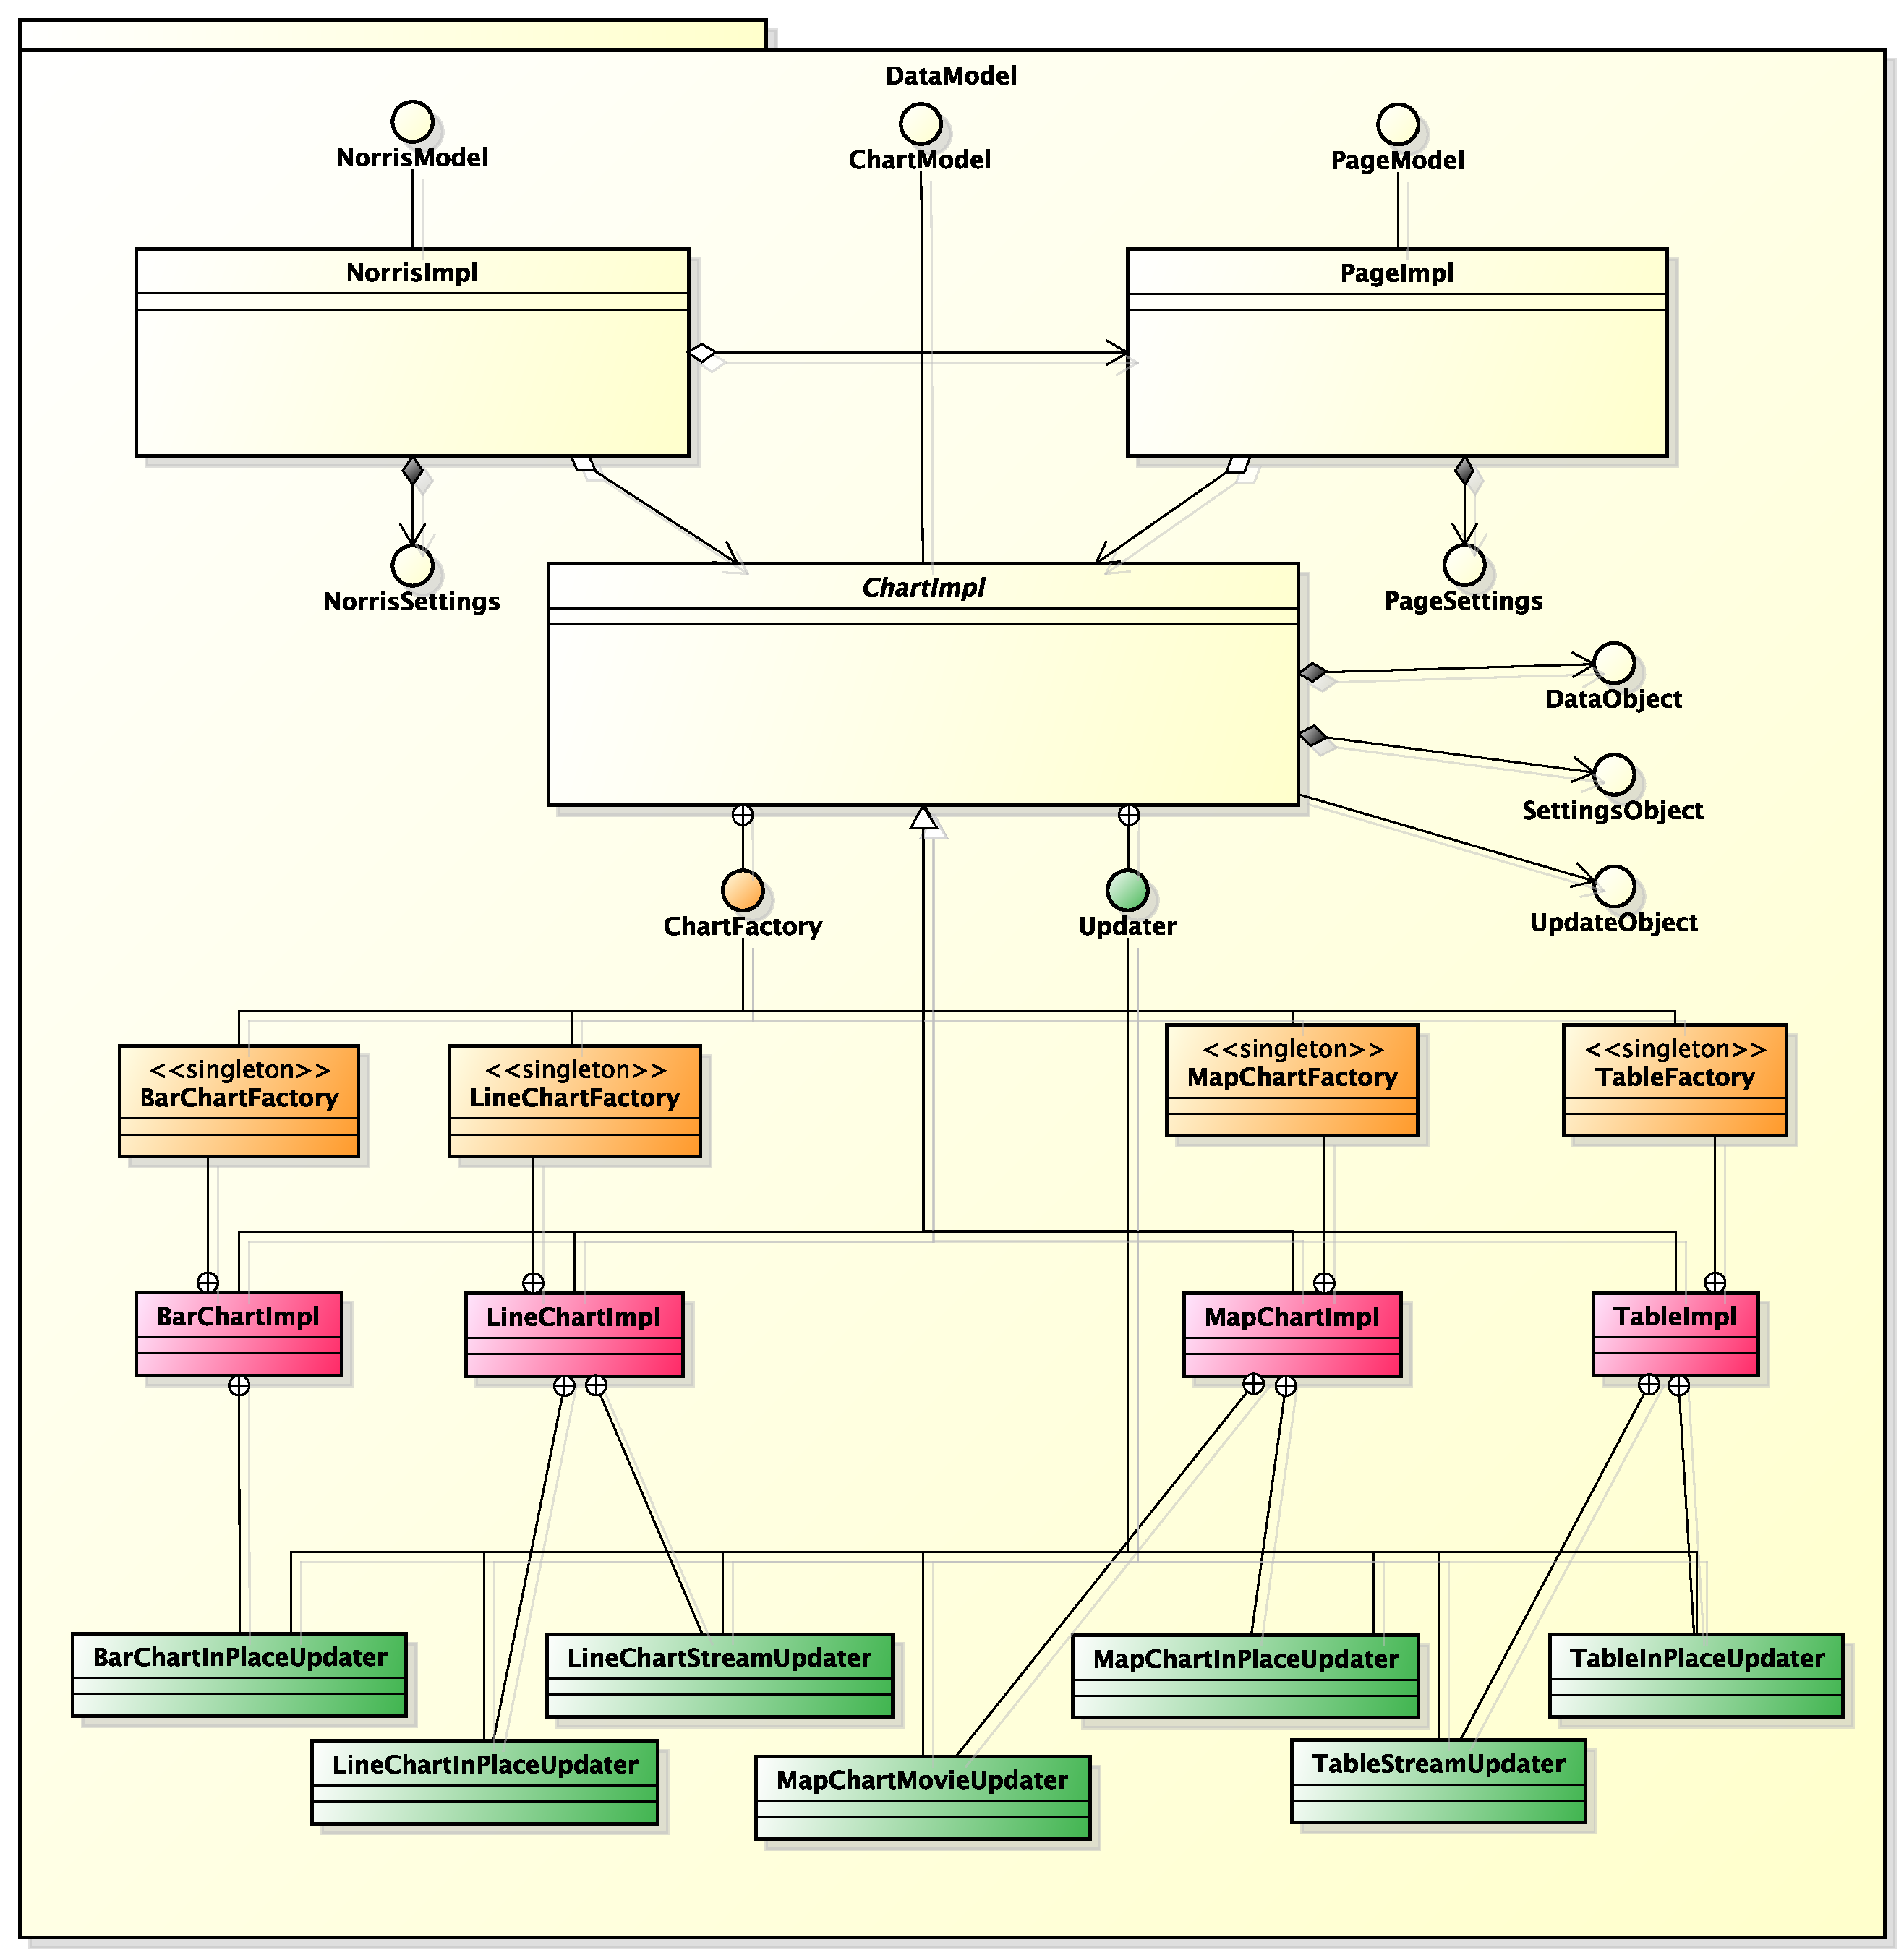
\includegraphics[scale=0.5]{DefinizioneDiProdotto/Pics/Classi/Norris--DataModel}
				\caption{Norris::DataModel}
			\end{figure}
		}
	

			\begin{itemize}
			\item \textbf{Nome:} DataModel
			\item \textbf{Tipo:} package
			
			\item \textbf{Descrizione:} DataModel è il package che astrae un’istanza di Norris. Al suo interno vi sono le informazioni relative alla struttura di grafici e pagine, assieme alle rispettive impostazioni. Inoltre vengono fissate le regole con le quali grafici e pagine vengono composti assieme per formare un’istanza di Norris. Il DataModel fornisce i metodi per inserire i dati e configurare le impostazioni. Fornisce inoltre dei metodi per ottenere i valori di queste ultime, in modo da poterle riutilizzare per un altro grafico o pagina. Infine sono presenti le classi che permettono che vengano memorizzate le informazioni inerenti l’autenticazione.

			\end{itemize}

			
			\level{4}[NorrisChart]{Norris::DataModel::NorrisChart}
			

		\IfFileExists{DefinizioneDiProdotto/Pics/Classi/Norris--DataModel--NorrisChart.pdf}{
			\begin{figure}[H]
				\centering
				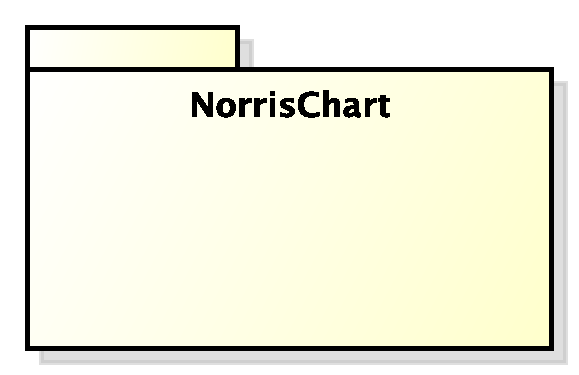
\includegraphics[scale=0.5]{DefinizioneDiProdotto/Pics/Classi/Norris--DataModel--NorrisChart}
				\caption{Norris::DataModel::NorrisChart}
			\end{figure}
		}
	

			\begin{itemize}
			\item \textbf{Nome:} NorrisChart
			\item \textbf{Tipo:} package
			
			\item \textbf{Descrizione:} NorrisChart è il package, le cui classi contengono i dati riguardanti i grafici con le relative impostazioni. Contiene le classi per ogni tipo di grafico, nelle quali sono implementati i metodi, per inserire i dati e configurare le impostazioni, e per ottenere tali valori. Inoltre, le classi di questo package mettono a disposizione le modalità di aggiornamento dei grafici.
			\end{itemize}

			
			\level{5}[BarChartImpl]{Norris::DataModel::NorrisChart::BarChartImpl}
			

		\IfFileExists{DefinizioneDiProdotto/Pics/Classi/Norris--DataModel--NorrisChart--BarChartImpl.pdf}{
			\begin{figure}[H]
				\centering
				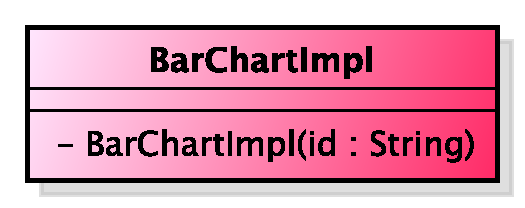
\includegraphics[scale=0.5]{DefinizioneDiProdotto/Pics/Classi/Norris--DataModel--NorrisChart--BarChartImpl}
				\caption{Norris::DataModel::NorrisChart::BarChartImpl}
			\end{figure}
		}
	
			
			\begin{itemize}
			\item \textbf{Nome:} BarChartImpl
			\item \textbf{Tipo:} classe
			
		\item \textbf{Estende:}
		ChartImpl
		\item \textbf{Astratta:}
		no
			\item \textbf{Visibilità:} package
			\item \textbf{Descrizione:} Questa classe rappresenta un grafico di tipo bar chart. Essa contiene al suo interno i dati (BarChartDataObject) e le impostazioni (BarChartSettingsObject) relativi al grafico. Inoltre contiene la classe BarChartInPlaceUpdater, la quale implementa l'aggiornamento di tipo in place per il grafico in questione. Un'istanza della classe BarChartImpl viene creata dalla classe factory BarChartFactory.

			\item \textbf{Metodi:}
				\begin{itemize}
				\setlength{\itemsep}{5pt}
				
					\item[\ding{111}] {{--BarChartImpl(id : String)}} \\ [1mm] Questo metodo è il costruttore della classe. Esso è privato perchè non può esser creata una istanza se non dalla sua classe interna factory.
				\end{itemize}
		
			\end{itemize}

			
			\level{5}[BarChartFactory]{Norris::DataModel::NorrisChart::BarChartImpl::BarChartFactory}
			

		\IfFileExists{DefinizioneDiProdotto/Pics/Classi/Norris--DataModel--NorrisChart--BarChartImpl--BarChartFactory.pdf}{
			\begin{figure}[H]
				\centering
				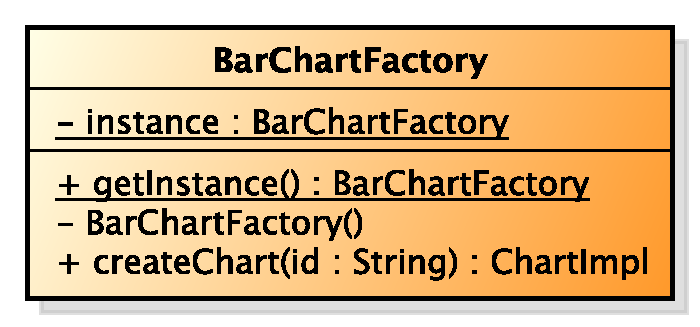
\includegraphics[scale=0.5]{DefinizioneDiProdotto/Pics/Classi/Norris--DataModel--NorrisChart--BarChartImpl--BarChartFactory}
				\caption{Norris::DataModel::NorrisChart::BarChartImpl::BarChartFactory}
			\end{figure}
		}
	
			
			\begin{itemize}
			\item \textbf{Nome:} BarChartFactory
			\item \textbf{Tipo:} classe
			
		\item \textbf{Astratta:}
		no
			\item \textbf{Visibilità:} private
			\item \textbf{Descrizione:} Questa classe si occupa della creazione di un grafico di tipo BarChartImpl. In particolare si occupa di configurare i dati e le impostazioni del grafico. Tale classe dispone di un blocco di inizializzazione statica che registra la sua istanza nel HashMap factories della classe ChartImpl non appena tale classe viene caricata.
			\item \textbf{Attributi:}
				\begin{itemize}
				\setlength{\itemsep}{5pt}
				
					\item[\ding{111}] \underline{--instance : BarChartFactory} \\ [1mm] Questo attributo è il riferimento all'unica istanza della classe.
				\end{itemize}
		
			\item \textbf{Metodi:}
				\begin{itemize}
				\setlength{\itemsep}{5pt}
				
					\item[\ding{111}] {\underline{+getInstance() : BarChartFactory}} \\ [1mm] Questo metodo permette di ottenere l'unica istanza esistente della classe.
					\item[\ding{111}] {{--BarChartFactory()}} \\ [1mm] Questo metodo è il costruttore della classe. Esso è privato perchè non si vuole permettere a nessuno di poter creare un’istanza se non utilizzando il metodo getInstance().

					\item[\ding{111}] {{+createChart(id : String) : ChartImpl}} \\ [1mm] Tale metodo ha il compito di creare la relativa specializzazione di ChartImpl. Esso può accedere al suo costruttore perchè questa classe factory è interna alla relativa classe BarChartImpl.
				\end{itemize}
		
			\end{itemize}

			
			\level{5}[BarChartInPlaceUpdater]{Norris::DataModel::NorrisChart::BarChartInPlaceUpdater}
			

		\IfFileExists{DefinizioneDiProdotto/Pics/Classi/Norris--DataModel--NorrisChart--BarChartInPlaceUpdater.pdf}{
			\begin{figure}[H]
				\centering
				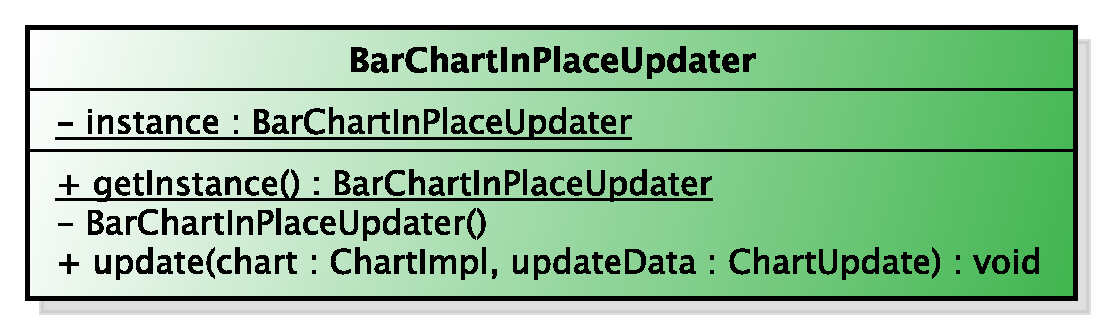
\includegraphics[scale=0.5]{DefinizioneDiProdotto/Pics/Classi/Norris--DataModel--NorrisChart--BarChartInPlaceUpdater}
				\caption{Norris::DataModel::NorrisChart::BarChartInPlaceUpdater}
			\end{figure}
		}
	
			
			\begin{itemize}
			\item \textbf{Nome:} BarChartInPlaceUpdater
			\item \textbf{Tipo:} classe
			
		\item \textbf{Astratta:}
		no
			\item \textbf{Visibilità:} package
			\item \textbf{Descrizione:} Questa classe si occupa di definire il metodo di aggiornamento in place per un grafico di tipo bar chart. In particolare modifica il DataObject contenuto in BarChartImpl tramite il metodo opportuno.
			\item \textbf{Attributi:}
				\begin{itemize}
				\setlength{\itemsep}{5pt}
				
					\item[\ding{111}] \underline{--instance : BarChartInPlaceUpdater} \\ [1mm] Questo attributo è il riferimento all'unica istanza della classe.
				\end{itemize}
		
			\item \textbf{Metodi:}
				\begin{itemize}
				\setlength{\itemsep}{5pt}
				
					\item[\ding{111}] {\underline{+getInstance() : BarChartInPlaceUpdater}} \\ [1mm] Questo metodo permette di ottenere l'unica istanza esistente della classe.
					\item[\ding{111}] {{--BarChartInPlaceUpdater()}} \\ [1mm] Questo metodo è il costruttore della classe.
					\item[\ding{111}] {{+update(chart : ChartImpl, updateData : ChartUpdate) : void}} \\ [1mm] Questo metodo permette di aggiornare il chart passato come primo parametro utilizzando i dati passati come secondo parametro.
				\end{itemize}
		
			\end{itemize}

			
			\level{5}[ChartImpl]{Norris::DataModel::NorrisChart::ChartImpl}
			

		\IfFileExists{DefinizioneDiProdotto/Pics/Classi/Norris--DataModel--NorrisChart--ChartImpl.pdf}{
			\begin{figure}[H]
				\centering
				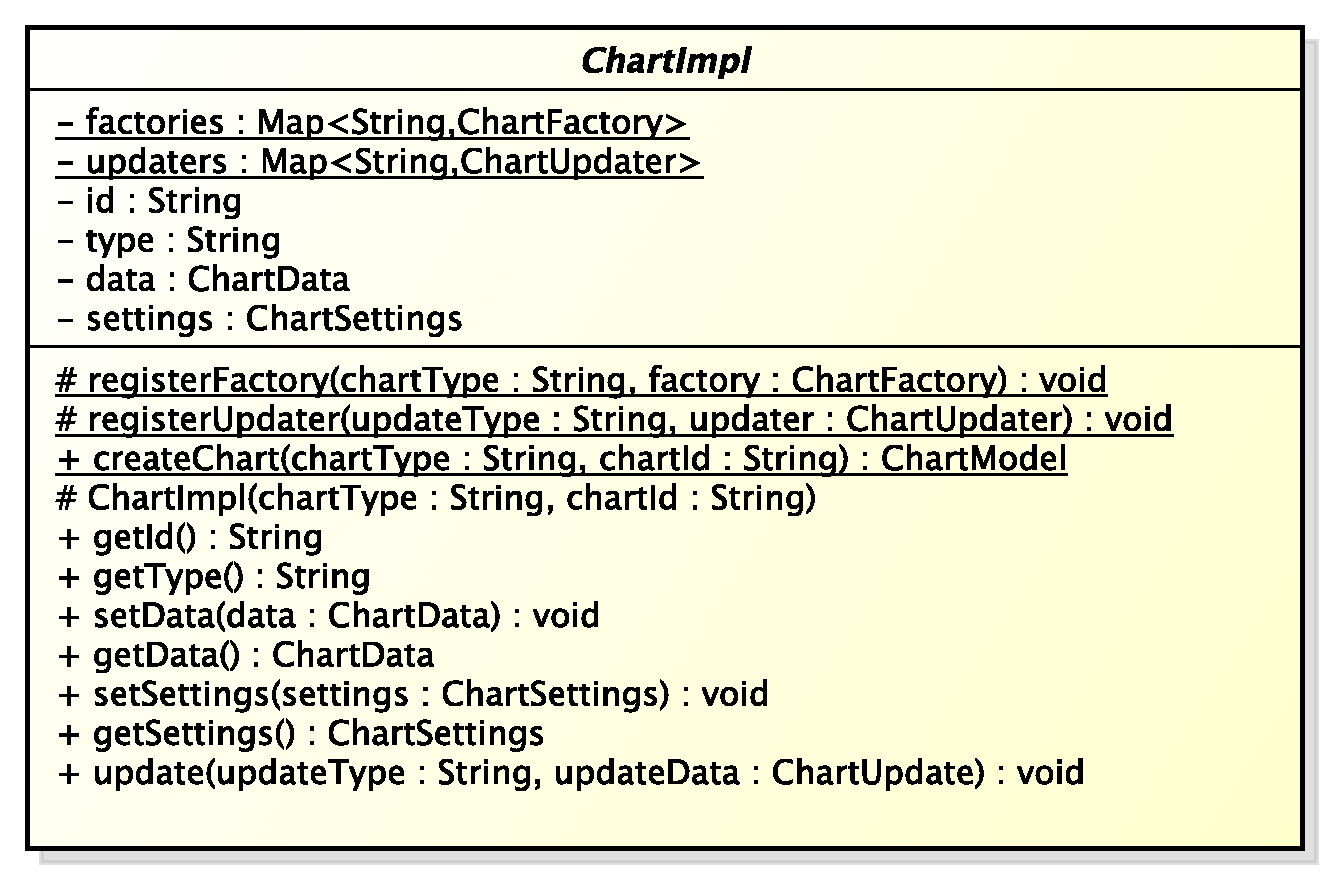
\includegraphics[scale=0.5]{DefinizioneDiProdotto/Pics/Classi/Norris--DataModel--NorrisChart--ChartImpl}
				\caption{Norris::DataModel::NorrisChart::ChartImpl}
			\end{figure}
		}
	
			
			\begin{itemize}
			\item \textbf{Nome:} ChartImpl
			\item \textbf{Tipo:} classe
			
		\item \textbf{Estende:}
		EventEmitter
		\item \textbf{Astratta:}
		si
			\item \textbf{Visibilità:} public
			\item \textbf{Descrizione:} Questa classe rappresenta un grafico generico e per questo motivo è una classe astratta. Essa contiene al suo interno i dati (ChartData) e le impostazioni (ChartSettings) relativi al grafico. Inoltre contiene l' interfaccia ChartFactory. Sono inoltre presenti due hashmap: la prima si occupa della corrispondenza tra le tipologie di grafico e le rispettive classi factory, la seconda invece si occupa della corrispondenza tra le varie tipologie di aggiornamento e la classe che implementa tale aggiornamento per un tipo specifico di grafico. ChartImpl ha una dipendenza verso l'interfaccia ChartUpdate, in quanto deve conoscere il tipo del pacchetto degli aggiornamenti.
			\item \textbf{Attributi:}
				\begin{itemize}
				\setlength{\itemsep}{5pt}
				
					\item[\ding{111}] \underline{--factories : Map<String,ChartFactory>} \\ [1mm] Questo attributo contiene le dipendenze necessarie per istanziare nuovi grafici. La chiave del HashMap rappresenta
					\item[\ding{111}] \underline{--updaters : Map<String,ChartUpdater>} \\ [1mm] Questo attributo contiene le dipendenze necessarie per aggiornare i grafici.
					\item[\ding{111}] {--id : String} \\ [1mm] Questo attributo consiste nell'id del grafico.
					\item[\ding{111}] {--type : String}
					\item[\ding{111}] {--data : ChartData} \\ [1mm] Questo attributo contiene i dati rappresentati dal grafico.
					\item[\ding{111}] {--settings : ChartSettings} \\ [1mm] Questo attributo contiene le impostazioni del grafico.
				\end{itemize}
		
			\item \textbf{Metodi:}
				\begin{itemize}
				\setlength{\itemsep}{5pt}
				
					\item[\ding{111}] {\underline{\#registerFactory(chartType : String, factory : ChartFactory) : void}} \\ [1mm] Tale metodo serve per registrare una certa factory al relativo chart nel HashMap della classe (factories). Tale metodo viene chiamato dalle classi factory interne ai vari ChartImpl con lo scopo di registrarsi come creatori di chart e poter quindi esser utilizzate per tale scopo.
					\item[\ding{111}] {\underline{\#registerUpdater(updateType : String, updater : ChartUpdater) : void}} \\ [1mm] Tale metodo serve per registrare un certo updater al relativo tipo di update nel MashMap della classe (updaters). Tale metodo viene invocato dalle classi Updater al loro caricamento per aggiungersi come updater.
					\item[\ding{111}] {\underline{+createChart(chartType : String, chartId : String) : ChartImpl}} \\ [1mm] Tale metodo non fa altro che creare il chart associato al parametro type e ritornare l’interfaccia ChartModel di tale istanza creata. Esso non fa altro che invocare il metodo chreateChart dela classe factory pesente nel HashMap factories con la chiave eguale al parametro type e ne ritornerà tale oggetto creato.
					\item[\ding{111}] {{\#ChartImpl(chartType : String, chartId : String)}} \\ [1mm] Questo metodo è il costruttore della classe. Esso è accessibile solamente alle sottoclassi per la creazione del sottoggetto.
					\item[\ding{111}] {{+getId() : String}} \\ [1mm] Questo metodo permette di ottenere l'id del grafico.
					\item[\ding{111}] {{+getType() : String}} \\ [1mm] Questo metodo permette di ottenere il tipo del grafico.
					\item[\ding{111}] {{+setData(data : ChartData) : void}} \\ [1mm] Questo metodo permette di impostare i dati del grafico.
					\item[\ding{111}] {{+getData() : ChartData}} \\ [1mm] Questo metodo permette di ottenere i dati del grafico.
					\item[\ding{111}] {{+setSettings(settings : ChartSettings) : void}} \\ [1mm] Questo metodo permette di impostare le opzioni del grafico.
					\item[\ding{111}] {{+getSettings() : ChartSettings}} \\ [1mm] Questo metodo permette di ottenere le opzioni del grafico.
					\item[\ding{111}] {{+update(updateType : String, updateData : ChartUpdate) : void}} \\ [1mm] Tale metodo ha il compito di aggiornare i chart utilizzando la tipologia di aggiornamento presente in updateType e il pacchetto di aggiornamento updateData. Esso non fa altro che invocare il metodo update dell’updater pesente nel HashMap updaters con la chiave eguale al parametro updateType e passargli come parametro il parametro ricevuto updateData ed i dati del chart che verranno modificati per riferimento.
				\end{itemize}
		
			\end{itemize}

			
			\level{5}[LineChartImpl]{Norris::DataModel::NorrisChart::LineChartImpl}
			

		\IfFileExists{DefinizioneDiProdotto/Pics/Classi/Norris--DataModel--NorrisChart--LineChartImpl.pdf}{
			\begin{figure}[H]
				\centering
				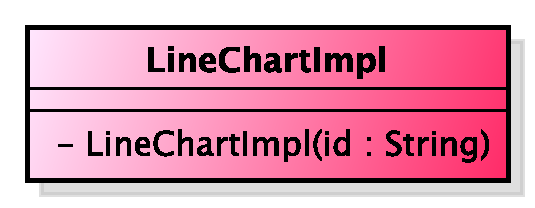
\includegraphics[scale=0.5]{DefinizioneDiProdotto/Pics/Classi/Norris--DataModel--NorrisChart--LineChartImpl}
				\caption{Norris::DataModel::NorrisChart::LineChartImpl}
			\end{figure}
		}
	
			
			\begin{itemize}
			\item \textbf{Nome:} LineChartImpl
			\item \textbf{Tipo:} classe
			
		\item \textbf{Estende:}
		ChartImpl
		\item \textbf{Astratta:}
		no
			\item \textbf{Visibilità:} package
			\item \textbf{Descrizione:} Questa classe rappresenta un grafico di tipo line chart. Essa contiene al suo interno i dati (LineChartDataObject) e le impostazioni (LineChartSettingsObject) relativi al grafico. Inoltre contiene le classi LineChartInPlaceUpdater e LineChartStreamUpdater, le quali implementano rispettivamente l'aggiornamento di tipo in place e stream per il grafico in questione. Un'istanza della classe LineChartImpl viene creata dalla classe factory LineChartFactory.
			\item \textbf{Metodi:}
				\begin{itemize}
				\setlength{\itemsep}{5pt}
				
					\item[\ding{111}] {{--LineChartImpl(id : String)}} \\ [1mm] Questo metodo è il costruttore della classe. Esso è privato perchè non può esser creata una istanza se non dalla sua classe interna factory.
				\end{itemize}
		
			\end{itemize}

			
			\level{5}[LineChartFactory]{Norris::DataModel::NorrisChart::LineChartImpl::LineChartFactory}
			

		\IfFileExists{DefinizioneDiProdotto/Pics/Classi/Norris--DataModel--NorrisChart--LineChartImpl--LineChartFactory.pdf}{
			\begin{figure}[H]
				\centering
				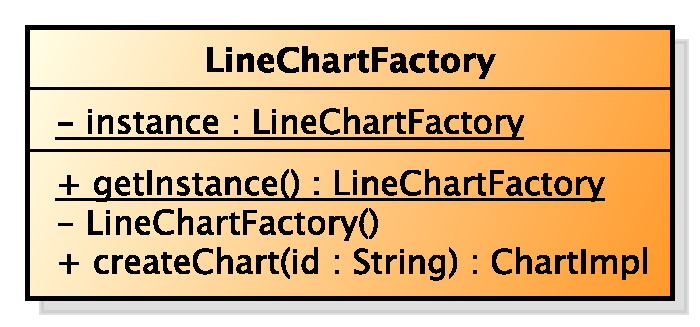
\includegraphics[scale=0.5]{DefinizioneDiProdotto/Pics/Classi/Norris--DataModel--NorrisChart--LineChartImpl--LineChartFactory}
				\caption{Norris::DataModel::NorrisChart::LineChartImpl::LineChartFactory}
			\end{figure}
		}
	
			
			\begin{itemize}
			\item \textbf{Nome:} LineChartFactory
			\item \textbf{Tipo:} classe
			
		\item \textbf{Astratta:}
		no
			\item \textbf{Visibilità:} private
			\item \textbf{Descrizione:} Questa classe si occupa della creazione di un grafico di tipo LineChartImpl. In particolare si occupa di configurare i dati e le impostazioni del grafico. Tale classe dispone di un blocco di inizializzazione statica che registra la sua istanza nel HashMap factories della classe ChartImpl non appena tale classe viene caricata.
			\item \textbf{Attributi:}
				\begin{itemize}
				\setlength{\itemsep}{5pt}
				
					\item[\ding{111}] \underline{--instance : LineChartFactory} \\ [1mm] Questo attributo è il riferimento all'unica istanza della classe.
				\end{itemize}
		
			\item \textbf{Metodi:}
				\begin{itemize}
				\setlength{\itemsep}{5pt}
				
					\item[\ding{111}] {\underline{+getInstance() : LineChartFactory}} \\ [1mm] Questo metodo permette di ottenere l'unica istanza esistente della classe.
					\item[\ding{111}] {{--LineChartFactory()}} \\ [1mm] Questo metodo è il costruttore della classe. Esso è privato perchè non si vuole permettere a nessuno di poter creare un’istanza se non utilizzando il metodo getInstance().

					\item[\ding{111}] {{+createChart(id : String) : ChartImpl}} \\ [1mm] Tale metodo ha il compito di creare la relativa specializzazione di ChartImpl. Esso può accedere al suo costruttore perchè questa classe factory è interna alla relativa classe BarChartImpl.
				\end{itemize}
		
			\end{itemize}

			
			\level{5}[LineChartInPlaceUpdater]{Norris::DataModel::NorrisChart::LineChartInPlaceUpdater}
			

		\IfFileExists{DefinizioneDiProdotto/Pics/Classi/Norris--DataModel--NorrisChart--LineChartInPlaceUpdater.pdf}{
			\begin{figure}[H]
				\centering
				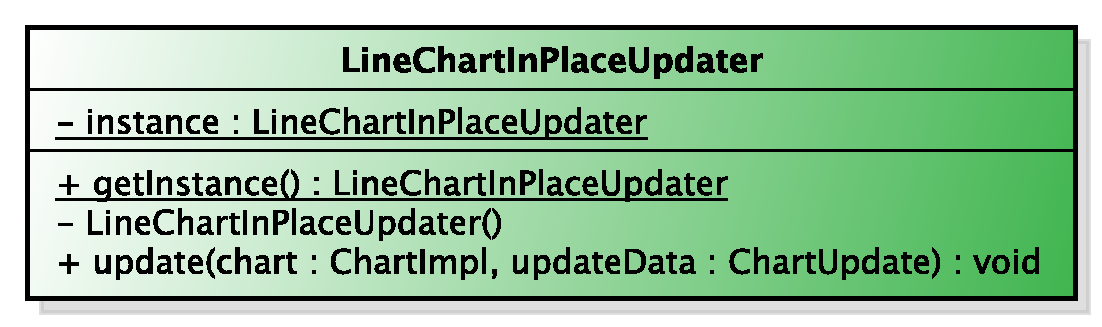
\includegraphics[scale=0.5]{DefinizioneDiProdotto/Pics/Classi/Norris--DataModel--NorrisChart--LineChartInPlaceUpdater}
				\caption{Norris::DataModel::NorrisChart::LineChartInPlaceUpdater}
			\end{figure}
		}
	
			
			\begin{itemize}
			\item \textbf{Nome:} LineChartInPlaceUpdater
			\item \textbf{Tipo:} classe
			
		\item \textbf{Astratta:}
		no
			\item \textbf{Visibilità:} package
			\item \textbf{Descrizione:} Questa classe si occupa di definire il metodo di aggiornamento in place per un grafico di tipo line chart. In particolare modifica il DataObject contenuto in LineChartImpl tramite il metodo opportuno.
			\item \textbf{Attributi:}
				\begin{itemize}
				\setlength{\itemsep}{5pt}
				
					\item[\ding{111}] \underline{--instance : LineChartInPlaceUpdater} \\ [1mm] Questo attributo è il riferimento all'unica istanza della classe.
				\end{itemize}
		
			\item \textbf{Metodi:}
				\begin{itemize}
				\setlength{\itemsep}{5pt}
				
					\item[\ding{111}] {\underline{+getInstance() : LineChartInPlaceUpdater}} \\ [1mm] Questo metodo permette di ottenere l'unica istanza esistente della classe.
					\item[\ding{111}] {{--LineChartInPlaceUpdater()}} \\ [1mm] Questo metodo è il costruttore della classe.
					\item[\ding{111}] {{+update(chart : ChartImpl, updateData : ChartUpdate) : void}} \\ [1mm] Questo metodo permette di aggiornare il chart passato come primo parametro utilizzando i dati passati come secondo parametro.
				\end{itemize}
		
			\end{itemize}

			
			\level{5}[LineChartStreamUpdater]{Norris::DataModel::NorrisChart::LineChartStreamUpdater}
			

		\IfFileExists{DefinizioneDiProdotto/Pics/Classi/Norris--DataModel--NorrisChart--LineChartStreamUpdater.pdf}{
			\begin{figure}[H]
				\centering
				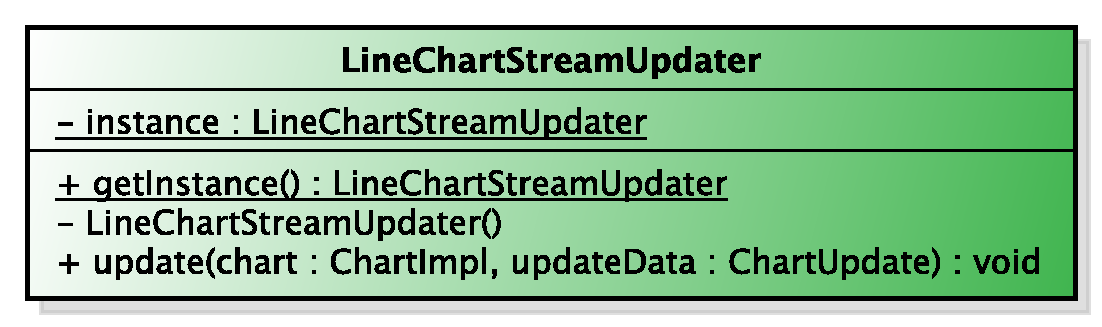
\includegraphics[scale=0.5]{DefinizioneDiProdotto/Pics/Classi/Norris--DataModel--NorrisChart--LineChartStreamUpdater}
				\caption{Norris::DataModel::NorrisChart::LineChartStreamUpdater}
			\end{figure}
		}
	
			
			\begin{itemize}
			\item \textbf{Nome:} LineChartStreamUpdater
			\item \textbf{Tipo:} classe
			
		\item \textbf{Astratta:}
		no
			\item \textbf{Visibilità:} package
			\item \textbf{Descrizione:} Questa classe si occupa di definire il metodo di aggiornamento stream per un grafico di tipo line chart. In particolare modifica il DataObject contenuto in LineChartImpl tramite il metodo opportuno.
			\item \textbf{Attributi:}
				\begin{itemize}
				\setlength{\itemsep}{5pt}
				
					\item[\ding{111}] \underline{--instance : LineChartStreamUpdater} \\ [1mm] Questo attributo è il riferimento all'unica istanza della classe.
				\end{itemize}
		
			\item \textbf{Metodi:}
				\begin{itemize}
				\setlength{\itemsep}{5pt}
				
					\item[\ding{111}] {\underline{+getInstance() : LineChartStreamUpdater}} \\ [1mm] Questo metodo permette di ottenere l'unica istanza esistente della classe.
					\item[\ding{111}] {{--LineChartStreamUpdater()}} \\ [1mm] Questo metodo è il costruttore della classe.
					\item[\ding{111}] {{+update(chart : ChartImpl, updateData : ChartUpdate) : void}} \\ [1mm] Questo metodo permette di aggiornare il chart passato come primo parametro utilizzando i dati passati come secondo parametro.
				\end{itemize}
		
			\end{itemize}

			
			\level{5}[MapChartImpl]{Norris::DataModel::NorrisChart::MapChartImpl}
			

		\IfFileExists{DefinizioneDiProdotto/Pics/Classi/Norris--DataModel--NorrisChart--MapChartImpl.pdf}{
			\begin{figure}[H]
				\centering
				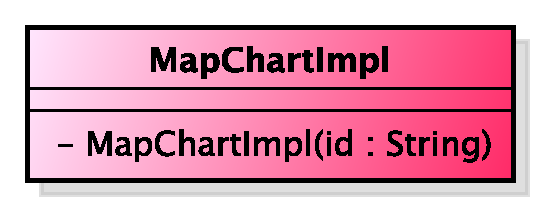
\includegraphics[scale=0.5]{DefinizioneDiProdotto/Pics/Classi/Norris--DataModel--NorrisChart--MapChartImpl}
				\caption{Norris::DataModel::NorrisChart::MapChartImpl}
			\end{figure}
		}
	
			
			\begin{itemize}
			\item \textbf{Nome:} MapChartImpl
			\item \textbf{Tipo:} classe
			
		\item \textbf{Estende:}
		ChartImpl
		\item \textbf{Astratta:}
		no
			\item \textbf{Visibilità:} package
			\item \textbf{Descrizione:} Questa classe rappresenta un grafico di tipo map chart. Essa contiene al suo interno i dati (MapChartDataObject) e le impostazioni (MapChartSettingsObject) relativi al grafico. Inoltre contiene le classi MapChartInPlaceUpdater e MapChartMovieUpdater, le quali implementano rispettivamente l'aggiornamento di tipo in place e movie per il grafico in questione. Un'istanza della classe MapChartImpl viene creata dalla classe factory MapChartFactory.
			\item \textbf{Metodi:}
				\begin{itemize}
				\setlength{\itemsep}{5pt}
				
					\item[\ding{111}] {{--MapChartImpl(id : String)}} \\ [1mm] Questo metodo è il costruttore della classe. Esso è privato perchè non può esser creata una istanza se non dalla sua classe interna factory.
				\end{itemize}
		
			\end{itemize}

			
			\level{5}[MapChartFactory]{Norris::DataModel::NorrisChart::MapChartImpl::MapChartFactory}
			

		\IfFileExists{DefinizioneDiProdotto/Pics/Classi/Norris--DataModel--NorrisChart--MapChartImpl--MapChartFactory.pdf}{
			\begin{figure}[H]
				\centering
				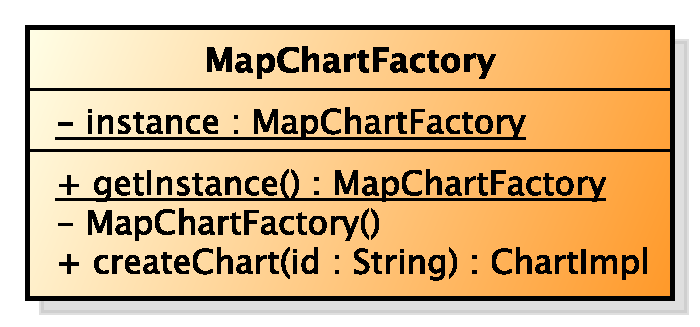
\includegraphics[scale=0.5]{DefinizioneDiProdotto/Pics/Classi/Norris--DataModel--NorrisChart--MapChartImpl--MapChartFactory}
				\caption{Norris::DataModel::NorrisChart::MapChartImpl::MapChartFactory}
			\end{figure}
		}
	
			
			\begin{itemize}
			\item \textbf{Nome:} MapChartFactory
			\item \textbf{Tipo:} classe
			
		\item \textbf{Astratta:}
		no
			\item \textbf{Visibilità:} private
			\item \textbf{Descrizione:} Questa classe si occupa della creazione di un grafico di tipo MapChartImpl. In particolare si occupa di configurare i dati e le impostazioni del grafico. Tale classe dispone di un blocco di inizializzazione statica che registra la sua istanza nel HashMap factories della classe ChartImpl non appena tale classe viene caricata.
			\item \textbf{Attributi:}
				\begin{itemize}
				\setlength{\itemsep}{5pt}
				
					\item[\ding{111}] \underline{--instance : MapChartFactory} \\ [1mm] Questo attributo è il riferimento all'unica istanza della classe.
				\end{itemize}
		
			\item \textbf{Metodi:}
				\begin{itemize}
				\setlength{\itemsep}{5pt}
				
					\item[\ding{111}] {\underline{+getInstance() : MapChartFactory}} \\ [1mm] Questo metodo permette di ottenere l'unica istanza esistente della classe.
					\item[\ding{111}] {{--MapChartFactory()}} \\ [1mm] Questo metodo è il costruttore della classe. Esso è privato perchè non si vuole permettere a nessuno di poter creare un’istanza se non utilizzando il metodo getInstance().

					\item[\ding{111}] {{+createChart(id : String) : ChartImpl}} \\ [1mm] Tale metodo ha il compito di creare la relativa specializzazione di ChartImpl. Esso può accedere al suo costruttore perchè questa classe factory è interna alla relativa classe BarChartImpl.
				\end{itemize}
		
			\end{itemize}

			
			\level{5}[MapChartInPlaceUpdater]{Norris::DataModel::NorrisChart::MapChartInPlaceUpdater}
			

		\IfFileExists{DefinizioneDiProdotto/Pics/Classi/Norris--DataModel--NorrisChart--MapChartInPlaceUpdater.pdf}{
			\begin{figure}[H]
				\centering
				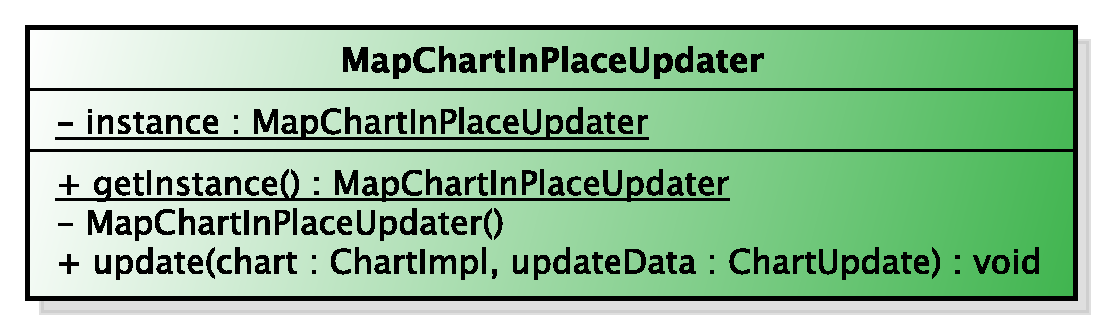
\includegraphics[scale=0.5]{DefinizioneDiProdotto/Pics/Classi/Norris--DataModel--NorrisChart--MapChartInPlaceUpdater}
				\caption{Norris::DataModel::NorrisChart::MapChartInPlaceUpdater}
			\end{figure}
		}
	
			
			\begin{itemize}
			\item \textbf{Nome:} MapChartInPlaceUpdater
			\item \textbf{Tipo:} classe
			
		\item \textbf{Astratta:}
		no
			\item \textbf{Visibilità:} package
			\item \textbf{Descrizione:} Questa classe si occupa di definire il metodo di aggiornamento in place per un grafico di tipo map chart. In particolare modifica il DataObject contenuto in MapChartImpl tramite il metodo opportuno.
			\item \textbf{Attributi:}
				\begin{itemize}
				\setlength{\itemsep}{5pt}
				
					\item[\ding{111}] \underline{--instance : MapChartInPlaceUpdater} \\ [1mm] Questo attributo è il riferimento all'unica istanza della classe.
				\end{itemize}
		
			\item \textbf{Metodi:}
				\begin{itemize}
				\setlength{\itemsep}{5pt}
				
					\item[\ding{111}] {\underline{+getInstance() : MapChartInPlaceUpdater}} \\ [1mm] Questo metodo permette di ottenere l'unica istanza esistente della classe.
					\item[\ding{111}] {{--MapChartInPlaceUpdater()}} \\ [1mm] Questo metodo è il costruttore della classe.
					\item[\ding{111}] {{+update(chart : ChartImpl, updateData : ChartUpdate) : void}} \\ [1mm] Questo metodo permette di aggiornare il chart passato come primo parametro utilizzando i dati passati come secondo parametro.
				\end{itemize}
		
			\end{itemize}

			
			\level{5}[MapChartMovieUpdater]{Norris::DataModel::NorrisChart::MapChartMovieUpdater}
			

		\IfFileExists{DefinizioneDiProdotto/Pics/Classi/Norris--DataModel--NorrisChart--MapChartMovieUpdater.pdf}{
			\begin{figure}[H]
				\centering
				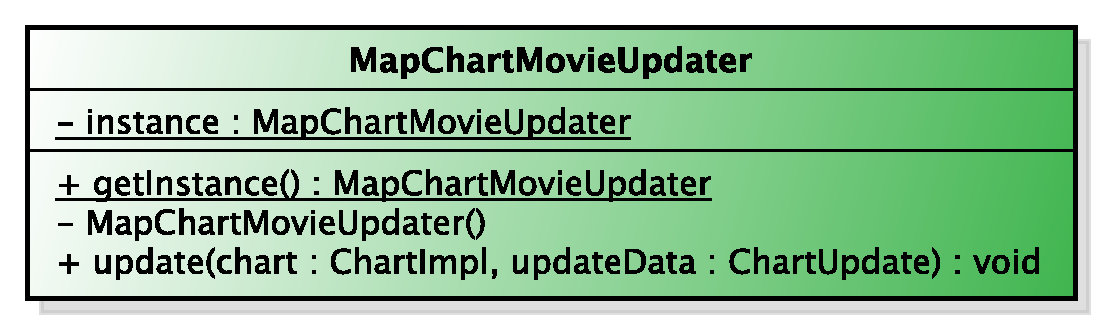
\includegraphics[scale=0.5]{DefinizioneDiProdotto/Pics/Classi/Norris--DataModel--NorrisChart--MapChartMovieUpdater}
				\caption{Norris::DataModel::NorrisChart::MapChartMovieUpdater}
			\end{figure}
		}
	
			
			\begin{itemize}
			\item \textbf{Nome:} MapChartMovieUpdater
			\item \textbf{Tipo:} classe
			
		\item \textbf{Astratta:}
		no
			\item \textbf{Visibilità:} package
			\item \textbf{Descrizione:} Questa classe si occupa di definire il metodo di aggiornamento movie per un grafico di tipo map chart. In particolare modifica il DataObject contenuto in MapChartImpl tramite il metodo opportuno.
			\item \textbf{Attributi:}
				\begin{itemize}
				\setlength{\itemsep}{5pt}
				
					\item[\ding{111}] \underline{--instance : MapChartMovieUpdater} \\ [1mm] Questo attributo è il riferimento all'unica istanza della classe.
				\end{itemize}
		
			\item \textbf{Metodi:}
				\begin{itemize}
				\setlength{\itemsep}{5pt}
				
					\item[\ding{111}] {\underline{+getInstance() : MapChartMovieUpdater}} \\ [1mm] Questo metodo permette di ottenere l'unica istanza esistente della classe.
					\item[\ding{111}] {{--MapChartMovieUpdater()}} \\ [1mm] Questo metodo è il costruttore della classe.
					\item[\ding{111}] {{+update(chart : ChartImpl, updateData : ChartUpdate) : void}} \\ [1mm] Questo metodo permette di aggiornare il chart passato come primo parametro utilizzando i dati passati come secondo parametro.
				\end{itemize}
		
			\end{itemize}

			
			\level{5}[TableImpl]{Norris::DataModel::NorrisChart::TableImpl}
			

		\IfFileExists{DefinizioneDiProdotto/Pics/Classi/Norris--DataModel--NorrisChart--TableImpl.pdf}{
			\begin{figure}[H]
				\centering
				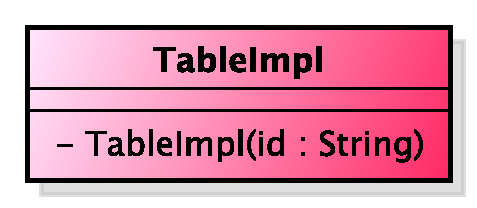
\includegraphics[scale=0.5]{DefinizioneDiProdotto/Pics/Classi/Norris--DataModel--NorrisChart--TableImpl}
				\caption{Norris::DataModel::NorrisChart::TableImpl}
			\end{figure}
		}
	
			
			\begin{itemize}
			\item \textbf{Nome:} TableImpl
			\item \textbf{Tipo:} classe
			
		\item \textbf{Estende:}
		ChartImpl
		\item \textbf{Astratta:}
		no
			\item \textbf{Visibilità:} package
			\item \textbf{Descrizione:} Questa classe rappresenta un grafico di tipo table. Essa contiene al suo interno i dati (TableDataObject) e le impostazioni (TableSettingsObject) relativi al grafico. Inoltre contiene le classi TableInPlaceUpdater e TableStreamUpdater, le quali implementano rispettivamente l'aggiornamento di tipo in place e stream per il grafico in questione. Un'istanza della classe TableImpl viene creata dalla classe factory TableFactory.
			\item \textbf{Metodi:}
				\begin{itemize}
				\setlength{\itemsep}{5pt}
				
					\item[\ding{111}] {{--TableImpl(id : String)}} \\ [1mm] Questo metodo è il costruttore della classe. Esso è privato perchè non può esser creata una istanza se non dalla sua classe interna factory.
				\end{itemize}
		
			\end{itemize}

			
			\level{5}[TableFactory]{Norris::DataModel::NorrisChart::TableImpl::TableFactory}
			

		\IfFileExists{DefinizioneDiProdotto/Pics/Classi/Norris--DataModel--NorrisChart--TableImpl--TableFactory.pdf}{
			\begin{figure}[H]
				\centering
				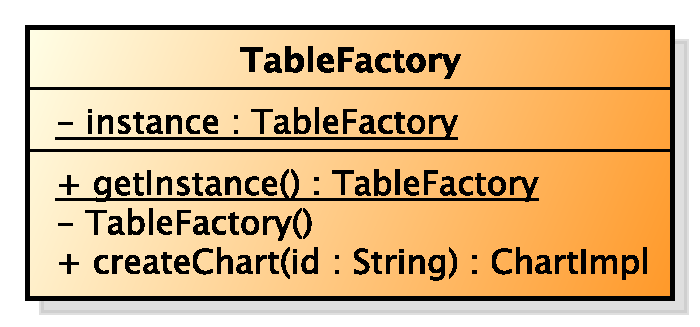
\includegraphics[scale=0.5]{DefinizioneDiProdotto/Pics/Classi/Norris--DataModel--NorrisChart--TableImpl--TableFactory}
				\caption{Norris::DataModel::NorrisChart::TableImpl::TableFactory}
			\end{figure}
		}
	
			
			\begin{itemize}
			\item \textbf{Nome:} TableFactory
			\item \textbf{Tipo:} classe
			
		\item \textbf{Astratta:}
		no
			\item \textbf{Visibilità:} private
			\item \textbf{Descrizione:} Questa classe si occupa della creazione di un grafico di tipo TableImpl. In particolare si occupa di configurare i dati e le impostazioni del grafico. Tale classe dispone di un blocco di inizializzazione statica che registra la sua istanza nel HashMap factories della classe ChartImpl non appena tale classe viene caricata.
			\item \textbf{Attributi:}
				\begin{itemize}
				\setlength{\itemsep}{5pt}
				
					\item[\ding{111}] \underline{--instance : TableFactory} \\ [1mm] Questo attributo è il riferimento all'unica istanza della classe.
				\end{itemize}
		
			\item \textbf{Metodi:}
				\begin{itemize}
				\setlength{\itemsep}{5pt}
				
					\item[\ding{111}] {\underline{+getInstance() : TableFactory}} \\ [1mm] Questo metodo permette di ottenere l'unica istanza esistente della classe.
					\item[\ding{111}] {{--TableFactory()}} \\ [1mm] Questo metodo è il costruttore della classe. Esso è privato perchè non si vuole permettere a nessuno di poter creare un’istanza se non utilizzando il metodo getInstance().
					\item[\ding{111}] {{+createChart(id : String) : ChartImpl}} \\ [1mm] Tale metodo ha il compito di creare la relativa specializzazione di ChartImpl. Esso può accedere al suo costruttore perchè questa classe factory è interna alla relativa classe BarChartImpl.
				\end{itemize}
		
			\end{itemize}

			
			\level{5}[TableInPlaceUpdater]{Norris::DataModel::NorrisChart::TableInPlaceUpdater}
			

		\IfFileExists{DefinizioneDiProdotto/Pics/Classi/Norris--DataModel--NorrisChart--TableInPlaceUpdater.pdf}{
			\begin{figure}[H]
				\centering
				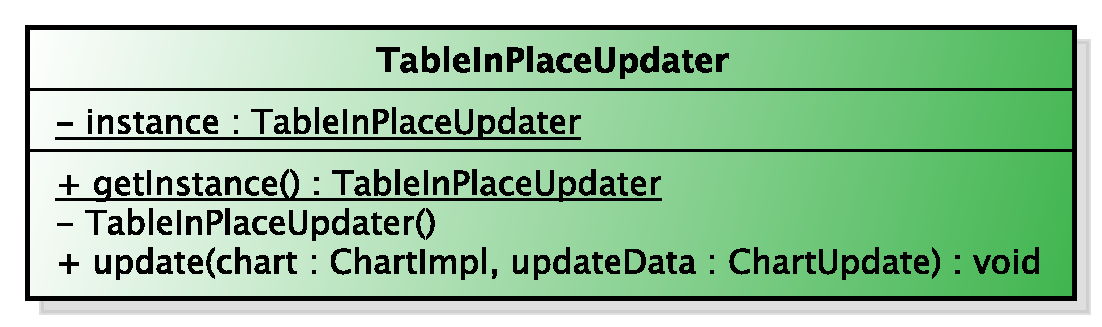
\includegraphics[scale=0.5]{DefinizioneDiProdotto/Pics/Classi/Norris--DataModel--NorrisChart--TableInPlaceUpdater}
				\caption{Norris::DataModel::NorrisChart::TableInPlaceUpdater}
			\end{figure}
		}
	
			
			\begin{itemize}
			\item \textbf{Nome:} TableInPlaceUpdater
			\item \textbf{Tipo:} classe
			
		\item \textbf{Astratta:}
		no
			\item \textbf{Visibilità:} package
			\item \textbf{Descrizione:} Questa classe si occupa di definire il metodo di aggiornamento in place per un grafico di tipo table. In particolare modifica il DataObject contenuto in Table tramite il metodo opportuno.
			\item \textbf{Attributi:}
				\begin{itemize}
				\setlength{\itemsep}{5pt}
				
					\item[\ding{111}] \underline{--instance : TableInPlaceUpdater} \\ [1mm] Questo attributo è il riferimento all'unica istanza della classe.
				\end{itemize}
		
			\item \textbf{Metodi:}
				\begin{itemize}
				\setlength{\itemsep}{5pt}
				
					\item[\ding{111}] {\underline{+getInstance() : TableInPlaceUpdater}} \\ [1mm] Questo metodo permette di ottenere l'unica istanza esistente della classe.
					\item[\ding{111}] {{--TableInPlaceUpdater()}} \\ [1mm] Questo metodo permette di aggiornare il chart passato come primo parametro utilizzando i dati passati come secondo parametro.
					\item[\ding{111}] {{+update(chart : ChartImpl, updateData : ChartUpdate) : void}} \\ [1mm] Questo metodo permette di aggiornare il chart passato come primo parametro utilizzando i dati passati come secondo parametro.
				\end{itemize}
		
			\end{itemize}

			
			\level{5}[TableStreamUpdater]{Norris::DataModel::NorrisChart::TableStreamUpdater}
			

		\IfFileExists{DefinizioneDiProdotto/Pics/Classi/Norris--DataModel--NorrisChart--TableStreamUpdater.pdf}{
			\begin{figure}[H]
				\centering
				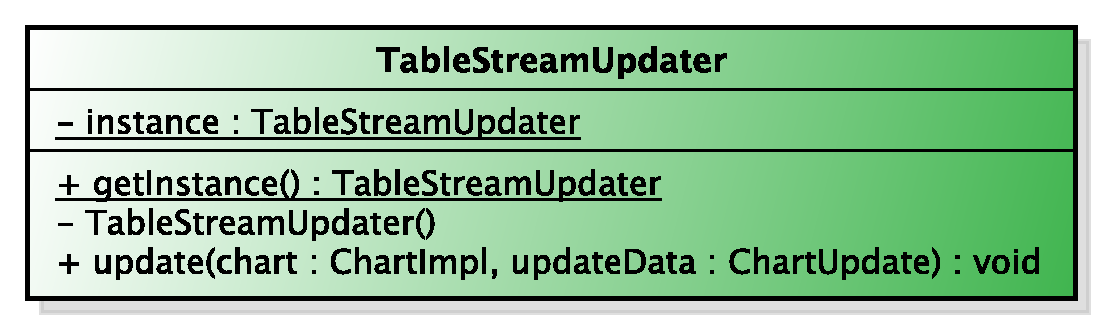
\includegraphics[scale=0.5]{DefinizioneDiProdotto/Pics/Classi/Norris--DataModel--NorrisChart--TableStreamUpdater}
				\caption{Norris::DataModel::NorrisChart::TableStreamUpdater}
			\end{figure}
		}
	
			
			\begin{itemize}
			\item \textbf{Nome:} TableStreamUpdater
			\item \textbf{Tipo:} classe
			
		\item \textbf{Astratta:}
		no
			\item \textbf{Visibilità:} package
			\item \textbf{Descrizione:} Questa classe si occupa di definire il metodo di aggiornamento stream per un grafico di tipo table. In particolare modifica il DataObject contenuto in Table tramite il metodo opportuno.
			\item \textbf{Attributi:}
				\begin{itemize}
				\setlength{\itemsep}{5pt}
				
					\item[\ding{111}] \underline{--instance : TableStreamUpdater} \\ [1mm] Questo attributo è il riferimento all'unica istanza della classe.
				\end{itemize}
		
			\item \textbf{Metodi:}
				\begin{itemize}
				\setlength{\itemsep}{5pt}
				
					\item[\ding{111}] {\underline{+getInstance() : TableStreamUpdater}} \\ [1mm] Questo metodo permette di ottenere l'unica istanza esistente della classe.
					\item[\ding{111}] {{--TableStreamUpdater()}} \\ [1mm] Questo metodo è il costruttore della classe.
					\item[\ding{111}] {{+update(chart : ChartImpl, updateData : ChartUpdate) : void}} \\ [1mm] Questo metodo permette di aggiornare il chart passato come primo parametro utilizzando i dati passati come secondo parametro.
				\end{itemize}
		
			\end{itemize}

			
			\level{5}[NorrisImpl]{Norris::DataModel::NorrisImpl}
			

		\IfFileExists{DefinizioneDiProdotto/Pics/Classi/Norris--DataModel--NorrisImpl.pdf}{
			\begin{figure}[H]
				\centering
				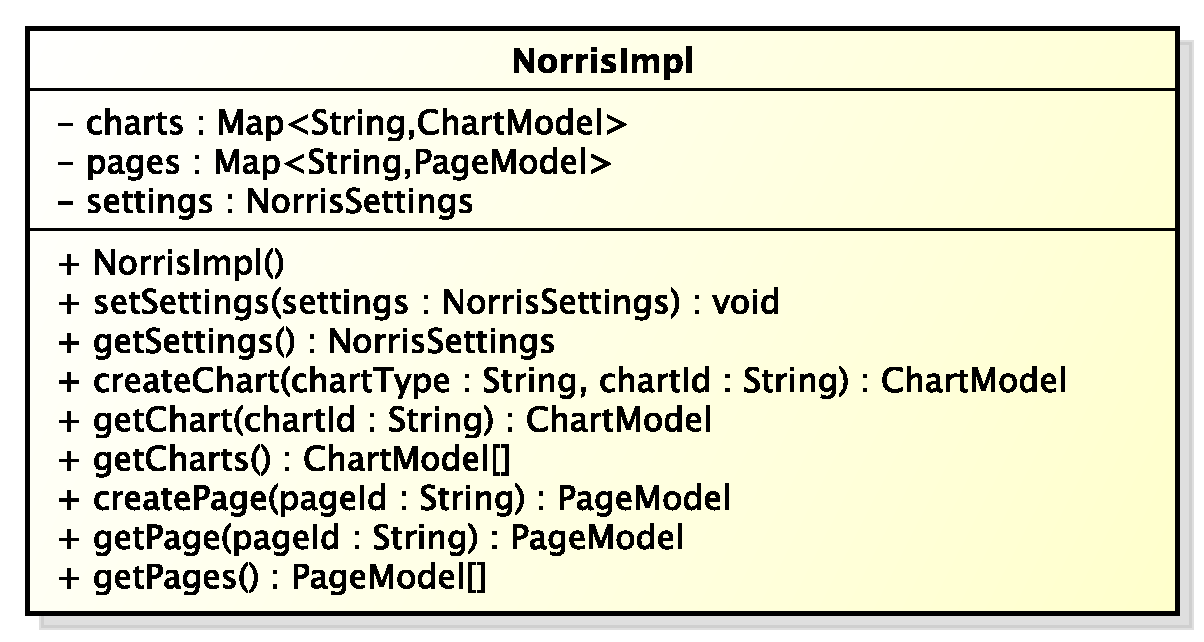
\includegraphics[scale=0.5]{DefinizioneDiProdotto/Pics/Classi/Norris--DataModel--NorrisImpl}
				\caption{Norris::DataModel::NorrisImpl}
			\end{figure}
		}
	
			
			\begin{itemize}
			\item \textbf{Nome:} NorrisImpl
			\item \textbf{Tipo:} classe
			
		\item \textbf{Estende:}
		EventEmitter
		\item \textbf{Astratta:}
		no
			\item \textbf{Visibilità:} public
			\item \textbf{Descrizione:} NorrisImpl implementa l'interfaccia NorrisModel e rappresenta il modello di un'istanza di Norris. Essa contiene al suo interno dei grafici (ChartImpl), delle pagine (PageImpl) e le impostazioni relative all'istanza di Norris. Tra queste ci sono le funzioni di autenticazione.
			\item \textbf{Attributi:}
				\begin{itemize}
				\setlength{\itemsep}{5pt}
				
					\item[\ding{111}] {--charts : Map<String,ChartImpl>} \\ [1mm] Questo attributo consiste nell'insieme dei grafici presenti nell'istanza di Norris.
					\item[\ding{111}] {--pages : Map<String,PageImpl>}
					\item[\ding{111}] {--settings : NorrisSettings} \\ [1mm] Questo attributo consiste nelle opzioni dell'istanza di Norris.
				\end{itemize}
		
			\item \textbf{Metodi:}
				\begin{itemize}
				\setlength{\itemsep}{5pt}
				
					\item[\ding{111}] {{+NorrisImpl(settings : NorrisSettings)}} \\ [1mm] Questo metodo è il costruttore della classe.
					\item[\ding{111}] {{+getSettings() : NorrisSettings}} \\ [1mm] Questo metodo permette di ottenere le impostazioni relative all'istanza di Norris.
					\item[\ding{111}] {{+createChart(chartType : String, chartId : String) : ChartImpl}} \\ [1mm] Questo metodo permette di creare un nuovo grafico e di aggiungerlo all'istanza di Norris.
					\item[\ding{111}] {{+getChart(chartId : String) : ChartImpl}} \\ [1mm] Questo metodo permette di ottenere un grafico presente nell'istanza di Norris dato il suo id.
					\item[\ding{111}] {{+getCharts() : ChartImpl}} \\ [1mm] Questo metodo permette di ottenere tutti i grafici presenti nell'istanza di Norris.
					\item[\ding{111}] {{+createPage(pageId : String) : PageImpl}} \\ [1mm] Questo metodo permette di creare una nuova pagina di aggiungerla all'istanza di Norris.
					\item[\ding{111}] {{+getPage(pageId : String) : PageImpl}} \\ [1mm] Questo metodo permette di ottenere una pagina presente nell'istanza di Norris dato il suo id.
					\item[\ding{111}] {{+getPages() : PageImpl[]}} \\ [1mm] Questo metodo permette di ottenere tutti le pagine presenti nell'istanza di Norris.
				\end{itemize}
		
			\end{itemize}

			
			\level{4}[NorrisPage]{Norris::DataModel::NorrisPage}
			

		\IfFileExists{DefinizioneDiProdotto/Pics/Classi/Norris--DataModel--NorrisPage.pdf}{
			\begin{figure}[H]
				\centering
				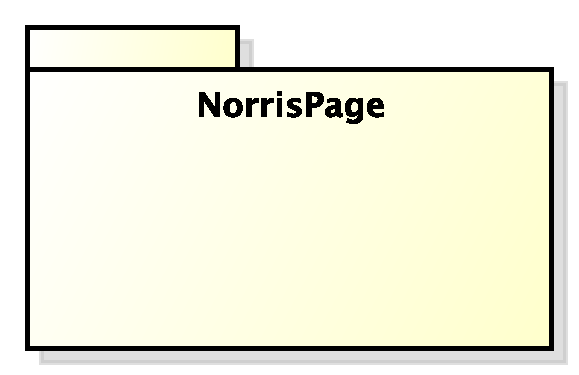
\includegraphics[scale=0.5]{DefinizioneDiProdotto/Pics/Classi/Norris--DataModel--NorrisPage}
				\caption{Norris::DataModel::NorrisPage}
			\end{figure}
		}
	

			\begin{itemize}
			\item \textbf{Nome:} NorrisPage
			\item \textbf{Tipo:} package
			
			\item \textbf{Descrizione:} NorrisPage è il package, le cui classi si occupano dell'aggiunta di grafici alle pagine e del settaggio delle impostazioni delle pagine.
			\end{itemize}

			
			\level{5}[PageImpl]{Norris::DataModel::NorrisPage::PageImpl}
			

		\IfFileExists{DefinizioneDiProdotto/Pics/Classi/Norris--DataModel--NorrisPage--PageImpl.pdf}{
			\begin{figure}[H]
				\centering
				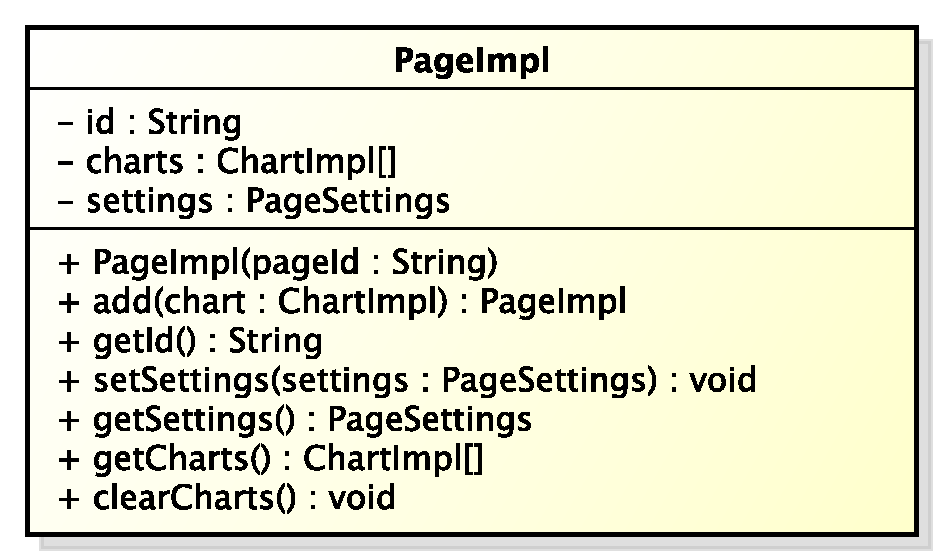
\includegraphics[scale=0.5]{DefinizioneDiProdotto/Pics/Classi/Norris--DataModel--NorrisPage--PageImpl}
				\caption{Norris::DataModel::NorrisPage::PageImpl}
			\end{figure}
		}
	
			
			\begin{itemize}
			\item \textbf{Nome:} PageImpl
			\item \textbf{Tipo:} classe
			
		\item \textbf{Astratta:}
		no
			\item \textbf{Visibilità:} public
			\item \textbf{Descrizione:} Questa classe rappresenta una pagina web. Essa contiene al suo interno dei grafici (ChartImpl) e le impostazioni della pagina web (PageSettingsObject).
			\item \textbf{Attributi:}
				\begin{itemize}
				\setlength{\itemsep}{5pt}
				
					\item[\ding{111}] {--id : String} \\ [1mm] Questo attributo consiste nell'id della pagina.
					\item[\ding{111}] {--charts : ChartImpl[]} \\ [1mm] Questo attributo consiste nell'insieme dei grafici contenuti nella pagina.
					\item[\ding{111}] {--settings : PageSettings} \\ [1mm] Questo attributo consiste nelle opzioni delle pagina rappresentata.
				\end{itemize}
		
			\item \textbf{Metodi:}
				\begin{itemize}
				\setlength{\itemsep}{5pt}
				
					\item[\ding{111}] {{+PageImpl(pageId : String)}} \\ [1mm] Questo metodo è il costruttore della classe. Il parametro rappresenta l'id che si vuole dare a atale pagina.
					\item[\ding{111}] {{+add(chart : ChartImpl) : PageImpl}} \\ [1mm] Questo metodo permette di aggiungere nuovi grafici alla pagina. Passando dunque come parametro un chart esso viene aggiunto alla pagina
					\item[\ding{111}] {{+getId() : String}} \\ [1mm] Questo metodo permette di ottenere l'id della pagina.
					\item[\ding{111}] {{+setSettings(settings : PageSettings) : void}} \\ [1mm] Questo metodo permette di impostare le opzioni della pagina.
					\item[\ding{111}] {{+getSettings() : PageSettings}} \\ [1mm] Questo metodo permette di ottenere le opzioni della pagina.
					\item[\ding{111}] {{+getCharts() : ChartImpl}} \\ [1mm] Questo metodo permette di ottenere la lista dei grafici contenuti nella pagina.
					\item[\ding{111}] {{+clearCharts() : void}} \\ [1mm] Questo metodo permette di togliere tutti i grafici contenuti nella pagina.
				\end{itemize}
		
			\end{itemize}

			
			\level{4}[InternalAPIManager]{Norris::InternalAPIManager}
			

		\IfFileExists{DefinizioneDiProdotto/Pics/Classi/Norris--InternalAPIManager.pdf}{
			\begin{figure}[H]
				\centering
				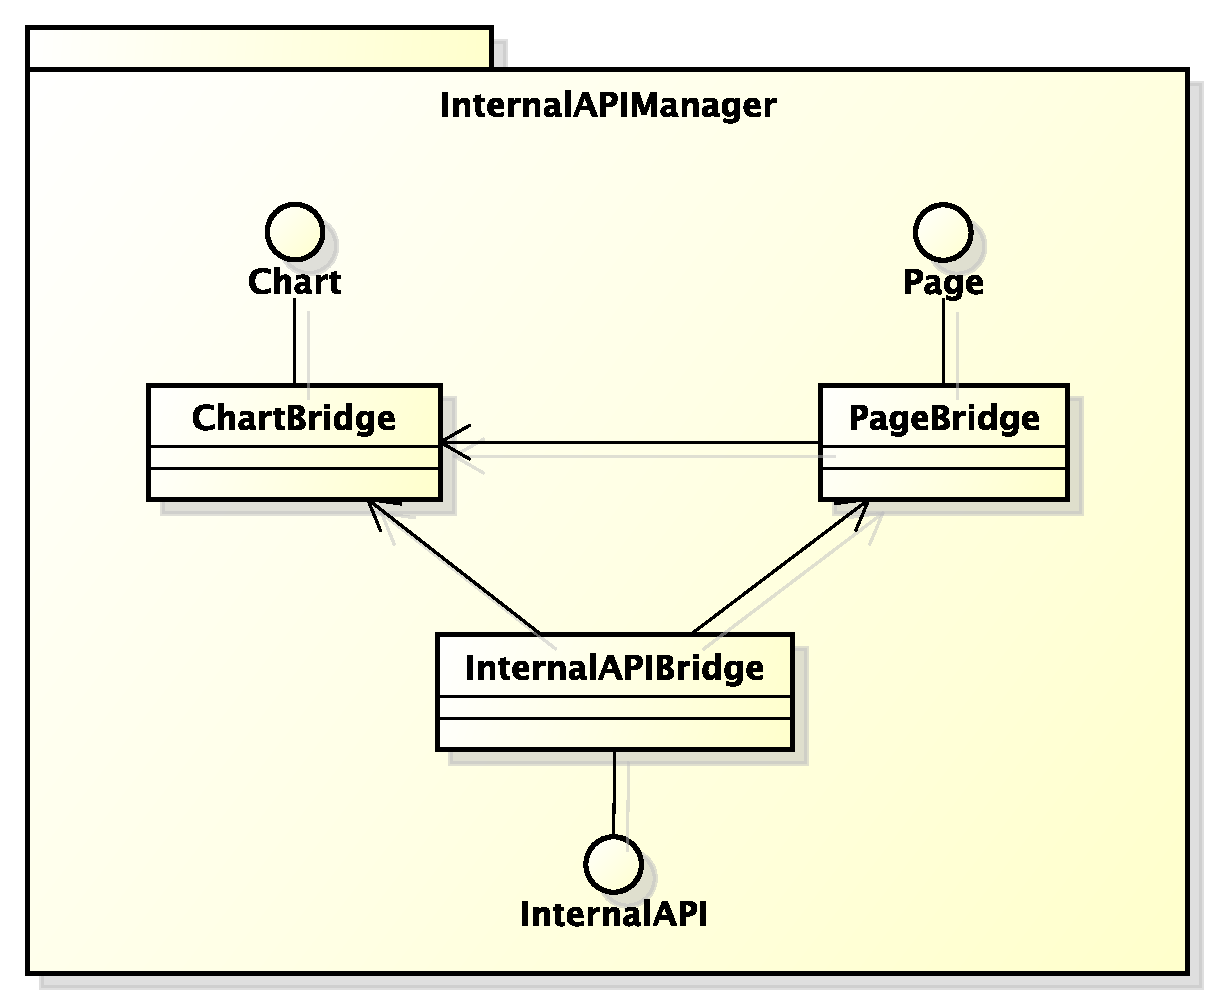
\includegraphics[scale=0.5]{DefinizioneDiProdotto/Pics/Classi/Norris--InternalAPIManager}
				\caption{Norris::InternalAPIManager}
			\end{figure}
		}
	

			\begin{itemize}
			\item \textbf{Nome:} InternalAPIManager
			\item \textbf{Tipo:} package
			
			\item \textbf{Descrizione:} InternalAPIManager è un package le cui classi si occupano di creare ed aggiornare grafici, creare pagine, aggiungere dei grafici ad esse o all'istanza di Norris e scegliere le varie impostazioni riguardanti grafici, pagine o istanze. Inoltre, forniscono le funzioni di autenticazione.
			\end{itemize}

			
			\level{5}[ChartBridge]{Norris::InternalAPIManager::ChartBridge}
			

		\IfFileExists{DefinizioneDiProdotto/Pics/Classi/Norris--InternalAPIManager--ChartBridge.pdf}{
			\begin{figure}[H]
				\centering
				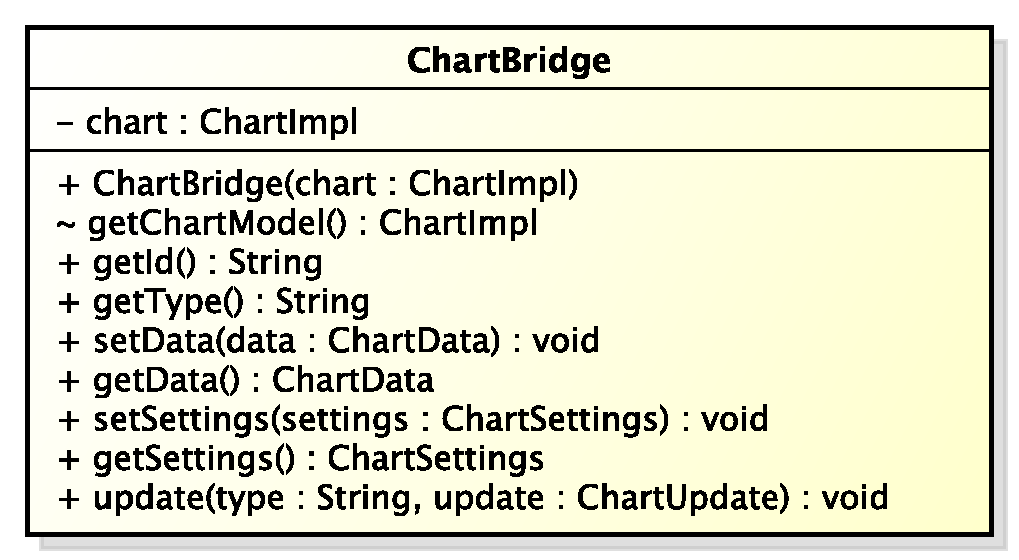
\includegraphics[scale=0.5]{DefinizioneDiProdotto/Pics/Classi/Norris--InternalAPIManager--ChartBridge}
				\caption{Norris::InternalAPIManager::ChartBridge}
			\end{figure}
		}
	
			
			\begin{itemize}
			\item \textbf{Nome:} ChartBridge
			\item \textbf{Tipo:} classe
			
		\item \textbf{Astratta:}
		no
			\item \textbf{Visibilità:} package
			\item \textbf{Descrizione:} ChartBridge implementa l'interfaccia Chart. Si occupa di inoltrare al modello dei dati le richieste di modifica delle impostazioni e le richieste di aggiornamento dei grafici.
			\item \textbf{Attributi:}
				\begin{itemize}
				\setlength{\itemsep}{5pt}
				
					\item[\ding{111}] {--chart : ChartImpl} \\ [1mm] Questo attributo è il riferimento all'istanza del chart rappresentato.
				\end{itemize}
		
			\item \textbf{Metodi:}
				\begin{itemize}
				\setlength{\itemsep}{5pt}
				
					\item[\ding{111}] {{+ChartBridge(chart : ChartImpl)}} \\ [1mm] Questo metodo è il costruttore della classe. esso salva il parametro nell'attributo chart.
					\item[\ding{111}] {{\(\sim\)getChartModel() : ChartImpl}} \\ [1mm] Questo metodo permette di ottenere il riferimento al chart rappresentato. Esso ritornerà il campo privato
					\item[\ding{111}] {{+getId() : String}} \\ [1mm] Questo metodo permette di ottenere l'id del chart rappresentato. Esso dovrà reperire tale informazione dal modello dei dati sfruttando l'attributo privato chart.
					\item[\ding{111}] {{+getType() : String}} \\ [1mm] Questo metodo permette di ottenere il tipo del chart rappresentato. Esso dovrà reperire tale informazione dal modello dei dati sfruttando l'attributo privato chart.
					\item[\ding{111}] {{+setData(data : ChartData) : void}} \\ [1mm] Questo metodo permette di impostare i dati del chart rappresentato.
					\item[\ding{111}] {{+getData() : ChartData}} \\ [1mm] Questo metodo permette di ottenere i dati del chart rappresentato. Esso dovrà reperire tale informazione dal modello dei dati sfruttando l'attributo privato chart.
					\item[\ding{111}] {{+setSettings(settings : ChartSettings) : void}} \\ [1mm] Questo metodo permette di impostare le opzioni del chart rappresentato.
					\item[\ding{111}] {{+getSettings() : ChartSettings}} \\ [1mm] Questo metodo permette di ottenere le opzioni del chart rappresentato. Esso dovrà reperire tale informazione dal modello dei dati sfruttando l'attributo privato chart.
					\item[\ding{111}] {{+update(type : String, update : ChartUpdate) : void}} \\ [1mm] Questo metodo permette di aggiornare il chart rappresentato secondo gli aggiornamenti previsti.
				\end{itemize}
		
			\end{itemize}

			
			\level{5}[NorrisBridge]{Norris::InternalAPIManager::NorrisBridge}
			

		\IfFileExists{DefinizioneDiProdotto/Pics/Classi/Norris--InternalAPIManager--NorrisBridge.pdf}{
			\begin{figure}[H]
				\centering
				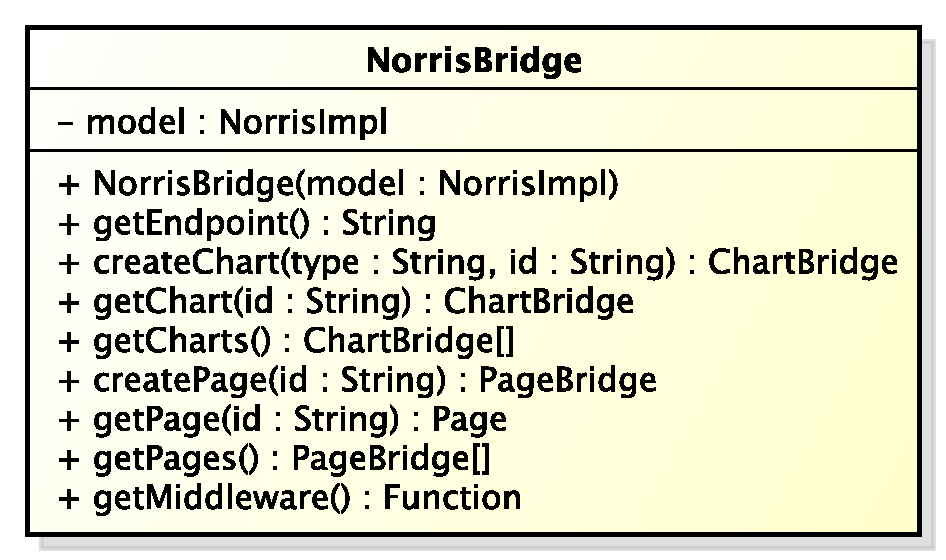
\includegraphics[scale=0.5]{DefinizioneDiProdotto/Pics/Classi/Norris--InternalAPIManager--NorrisBridge}
				\caption{Norris::InternalAPIManager::NorrisBridge}
			\end{figure}
		}
	
			
			\begin{itemize}
			\item \textbf{Nome:} NorrisBridge
			\item \textbf{Tipo:} classe
			
		\item \textbf{Astratta:}
		no
			\item \textbf{Visibilità:} public
			\item \textbf{Descrizione:} NorrisBridge implementa l'interfaccia Norris. Si occupa di inoltare al modello dei dati le richieste di modifica delle impostazioni e delle funzioni di autenticazione di un'istanza di Norris e le richieste di aggiunta di grafici e di pagine all'istanza stessa.
			\item \textbf{Attributi:}
				\begin{itemize}
				\setlength{\itemsep}{5pt}
				
					\item[\ding{111}] {--model : NorrisImpl} \\ [1mm] Questo attributo è il riferimento all'istanza di Norris rappresentata dalla classe.
				\end{itemize}
		
			\item \textbf{Metodi:}
				\begin{itemize}
				\setlength{\itemsep}{5pt}
				
					\item[\ding{111}] {{+NorrisBridge(model : NorrisImpl)}} \\ [1mm] Questo metodo è il costruttore della classe.
					\item[\ding{111}] {{+getEndpoint() : String}} \\ [1mm] Questo metodo permette di ottenere l'endpoint sul quale sono fornite le API. Esso reperirà tale informazione dal modello dei dati sfruttando l'attributo privato model.
					\item[\ding{111}] {{+createChart(type : String, id : String) : ChartBridge}} \\ [1mm] Questo metodo permette di creare un nuovo chart ed aggiungerlo all'istanza di Norris rappresentata.
					\item[\ding{111}] {{+getChart(id : String) : ChartBridge}} \\ [1mm] Questo metodo permette di ottenere un chart contenuto nell'istanza di Norris rappresentata tramite il suo id.
					\item[\ding{111}] {{+getCharts() : ChartBridge}} \\ [1mm] Questo metodo permette di ottenere l'insieme dei grafici presenti all'interno dell'istanza di Norris rappresentata.
					\item[\ding{111}] {{+createPage(id : String) : PageBridge}} \\ [1mm] Questo metodo permette di creare una nuova pagina ed aggiungerla all'istanza di Norris rappresentata.
					\item[\ding{111}] {{+getPage(id : String) : Page}} \\ [1mm] Questo metodo permette di ottenere una pagina contenuta nell'istanza di Norris rappresentata tramite il suo id.
					\item[\ding{111}] {{+getPages() : PageBridge[]}} \\ [1mm] Questo metodo permette di ottenere l'insieme delle pagine presenti all'interno dell'istanza di Norris rappresentata.
					\item[\ding{111}] {{+getMiddleware() : Function}} \\ [1mm] Questo metodo permette di ottenere un middleware per express, il quale consente di montare le pagine dell'instanza di Norris su un webserver.
				\end{itemize}
		
			\end{itemize}

			
			\level{5}[PageBridge]{Norris::InternalAPIManager::PageBridge}
			

		\IfFileExists{DefinizioneDiProdotto/Pics/Classi/Norris--InternalAPIManager--PageBridge.pdf}{
			\begin{figure}[H]
				\centering
				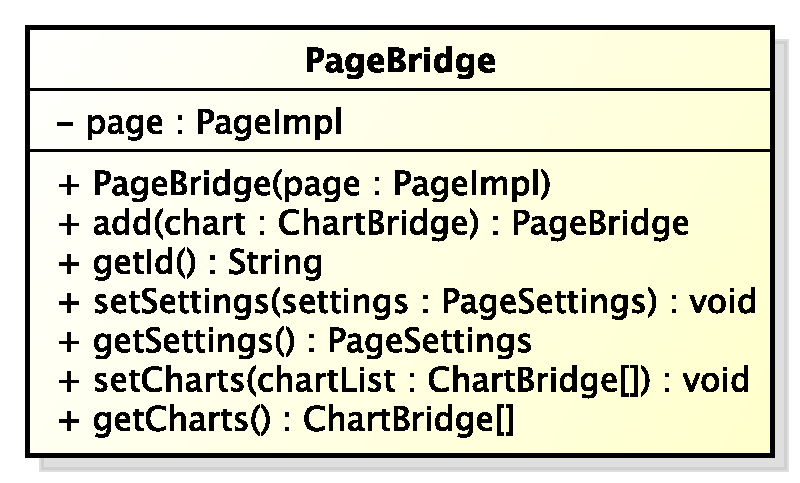
\includegraphics[scale=0.5]{DefinizioneDiProdotto/Pics/Classi/Norris--InternalAPIManager--PageBridge}
				\caption{Norris::InternalAPIManager::PageBridge}
			\end{figure}
		}
	
			
			\begin{itemize}
			\item \textbf{Nome:} PageBridge
			\item \textbf{Tipo:} classe
			
		\item \textbf{Astratta:}
		no
			\item \textbf{Visibilità:} package
			\item \textbf{Descrizione:} PageBridge implementa l'interfaccia Page. Si occupa di inoltare al modello dei dati le richieste di modifica delle impostazioni di una pagina e le richieste di aggiunta di grafici alla pagina stessa.
			\item \textbf{Attributi:}
				\begin{itemize}
				\setlength{\itemsep}{5pt}
				
					\item[\ding{111}] {--page : PageImpl} \\ [1mm] Questo attributo è un riferimento al tipo di pagina rappresentata.
				\end{itemize}
		
			\item \textbf{Metodi:}
				\begin{itemize}
				\setlength{\itemsep}{5pt}
				
					\item[\ding{111}] {{+PageBridge(page : PageImpl)}} \\ [1mm] Questo metodo è il costruttore della classe.	
					\item[\ding{111}] {{+add(chart : ChartBridge) : PageBridge}} \\ [1mm] Questo metodo permette di aggiungere nuovi chart alla pagina rappresentata.
					\item[\ding{111}] {{+getId() : String}} \\ [1mm] Questo metodo permette di ottenere l'id della pagina rappresentata.  Esso dovrà reperire tale informazione dal modello dei dati sfruttando l'attributo privato page.
					\item[\ding{111}] {{+setSettings(settings : PageSettings) : void}} \\ [1mm] Questo metodo permette di impostare le opzioni relative alla pagina rappresentata.
					\item[\ding{111}] {{+getSettings() : PageSettings}} \\ [1mm] Questo metodo permette di ottenere le opzioni della pagina rappresentata.  Esso dovrà reperire tale informazione dal modello dei dati sfruttando l'attributo privato page.
					\item[\ding{111}] {{+setCharts(chartList : ChartBridge[]) : void}} \\ [1mm] Questo metodo permette di impostare l'insieme dei chart contenuti nella pagina rappresentata.
					\item[\ding{111}] {{+getCharts() : ChartBridge[]}} \\ [1mm] Questo metodo permette di ottenere l'insieme dei chart contenuti nella pagina rappresentata. Esso dovrà reperire tale informazione dal modello dei dati sfruttando l'attributo privato page.
				\end{itemize}
		
			\end{itemize}

			
			\level{4}[ExternalAPIManager]{Norris::ExternalAPIManager}
			

		\IfFileExists{DefinizioneDiProdotto/Pics/Classi/Norris--ExternalAPIManager.pdf}{
			\begin{figure}[H]
				\centering
				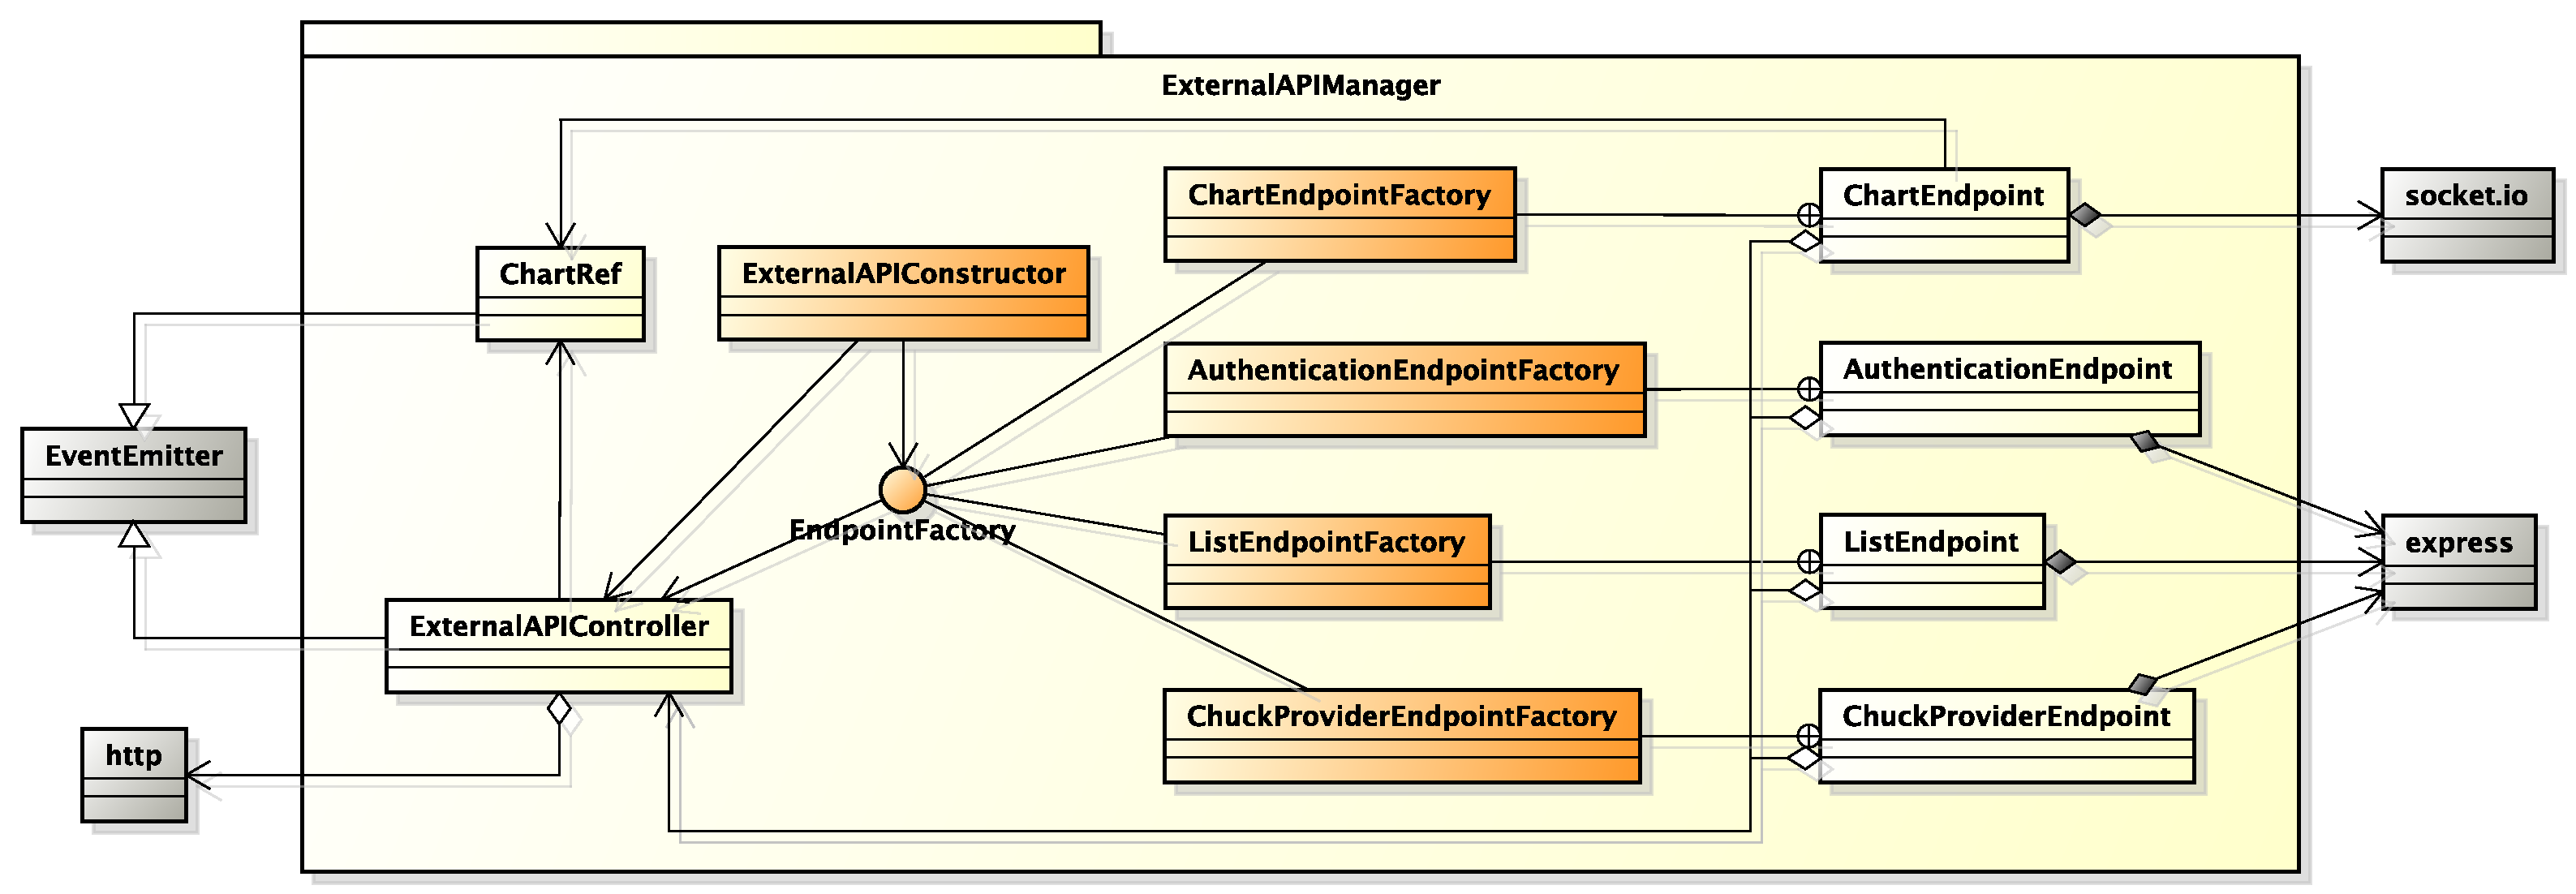
\includegraphics[scale=0.5]{DefinizioneDiProdotto/Pics/Classi/Norris--ExternalAPIManager}
				\caption{Norris::ExternalAPIManager}
			\end{figure}
		}
	

			\begin{itemize}
			\item \textbf{Nome:} ExternalAPIManager
			\item \textbf{Tipo:} package
			
			\item \textbf{Descrizione:} ExternalAPIManager è il package, le cui classi si occupano di implementare le funzionalità per: ottenere la lista dei grafici, ottenere un grafico con i relativi aggiornamenti ed effettuare login e logout. Inoltre, gestiscono la comunicazione con il websocket, tramite HTTP e canale Websocket.
			\end{itemize}

			
			\level{5}[AuthenticationEndpoint]{Norris::ExternalAPIManager::AuthenticationEndpoint}
			

		\IfFileExists{DefinizioneDiProdotto/Pics/Classi/Norris--ExternalAPIManager--AuthenticationEndpoint.pdf}{
			\begin{figure}[H]
				\centering
				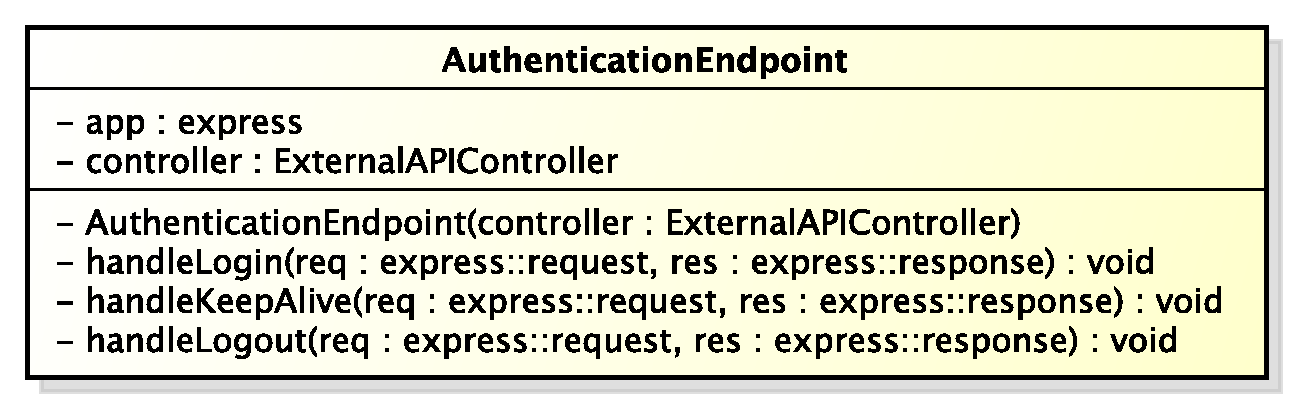
\includegraphics[scale=0.5]{DefinizioneDiProdotto/Pics/Classi/Norris--ExternalAPIManager--AuthenticationEndpoint}
				\caption{Norris::ExternalAPIManager::AuthenticationEndpoint}
			\end{figure}
		}
	
			
			\begin{itemize}
			\item \textbf{Nome:} AuthenticationEndpoint
			\item \textbf{Tipo:} classe
			
		\item \textbf{Astratta:}
		no
			\item \textbf{Visibilità:} package
			\item \textbf{Descrizione:} Questa classe si occupa di gestire l'autenticazione. In particolare si occupa di gestire le richieste di login e di logout, eseguendo le funzioni definite dallo sviluppatore e contenute in NorrisImpl.
			\item \textbf{Attributi:}
				\begin{itemize}
				\setlength{\itemsep}{5pt}
				
					\item[\ding{111}] {--controller : ExternalAPIController} \\ [1mm] Questo attributo è un riferimento all'oggetto che permette di ricavare informazioni sull'istanza di Norris.
				\end{itemize}
		
			\item \textbf{Metodi:}
				\begin{itemize}
				\setlength{\itemsep}{5pt}
				
					\item[\ding{111}] {{--AuthenticationEndpoint(controller : ExternalAPIController)}} \\ [1mm] Questo metodo è il costruttore della classe.
					\item[\ding{111}] {{--handleLogin(req : express::request, res : express::response) : void}} \\ [1mm] Questo metodo gestisce una richiesta di autenticazione. La richiesta HTTP ricevuta viene demandata all'ExternalAPIController che effettuerà il login.
					\item[\ding{111}] {{--handleKeepAlive(req : express::request, res : express::response) : void}} \\ [1mm] Questo metodo gestisce una richiesta per il rinnovo della sessione. La richiesta HTTP ricevuta viene demandata all'ExternalAPIController che effettuerà il mantenimento della sessione.
					\item[\ding{111}] {{--handleLogout(req : express::request, res : express::response) : void}} \\ [1mm] Questo metodo gestisce una richiesta per la terminazione della sessione. La richiesta HTTP ricevuta viene demandata all'ExternalAPIController che effettuerà il logout.
				\end{itemize}
		
			\end{itemize}

			
			\level{5}[AuthenticationEndpointFactory]{Norris::ExternalAPIManager::AuthenticationEndpoint::AuthenticationEndpointFactory}
			

		\IfFileExists{DefinizioneDiProdotto/Pics/Classi/Norris--ExternalAPIManager--AuthenticationEndpoint--AuthenticationEndpointFactory.pdf}{
			\begin{figure}[H]
				\centering
				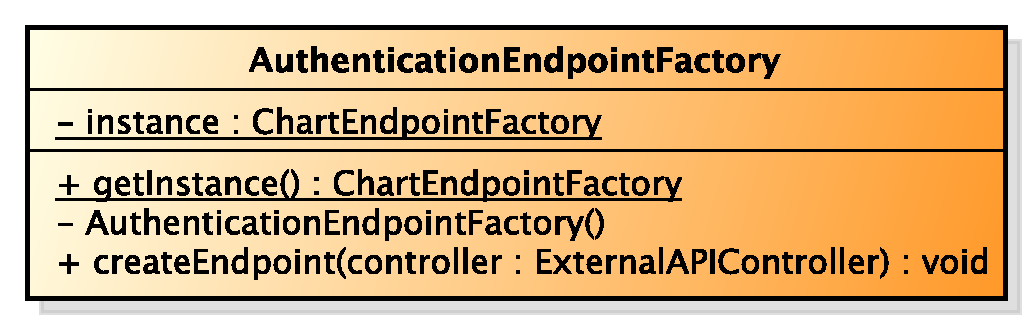
\includegraphics[scale=0.5]{DefinizioneDiProdotto/Pics/Classi/Norris--ExternalAPIManager--AuthenticationEndpoint--AuthenticationEndpointFactory}
				\caption{Norris::ExternalAPIManager::AuthenticationEndpoint::AuthenticationEndpointFactory}
			\end{figure}
		}
	
			
			\begin{itemize}
			\item \textbf{Nome:} AuthenticationEndpointFactory
			\item \textbf{Tipo:} classe
			
		\item \textbf{Astratta:}
		no
			\item \textbf{Visibilità:} private
			\item \textbf{Descrizione:} Questa classe si occupa della creazione di un endpoint di tipo AuthenticationEndpoint. Tale classe dispone di un blocco di inizializzazione statica che registra la sua istanza nell'array endpoints della classe ExternalAPIConstructor non appena tale classe viene caricata.
			\item \textbf{Attributi:}
				\begin{itemize}
				\setlength{\itemsep}{5pt}
				
					\item[\ding{111}] \underline{--instance : ChartEndpointFactory} \\ [1mm] Questo attributo è il riferimento all'unica istanza della classe.
				\end{itemize}
		
			\item \textbf{Metodi:}
				\begin{itemize}
				\setlength{\itemsep}{5pt}
				
					\item[\ding{111}] {\underline{+getInstance() : ChartEndpointFactory}} \\ [1mm] Questo metodo permette di ottenere l'unica istanza esistente della classe.
					\item[\ding{111}] {{--AuthenticationEndpointFactory()}} \\ [1mm] Questo metodo è il costruttore della classe. Esso è privato perchè non si vuole permettere a nessuno di poter creare un’istanza se non utilizzando il metodo getInstance().

					\item[\ding{111}] {{+createEndpoint(controller : ExternalAPIController) : void}} \\ [1mm] Questo metodo crea un'istanza della classe AuthenticationEndpoint.
				\end{itemize}
		
			\end{itemize}

			
			\level{5}[ChartEndpoint]{Norris::ExternalAPIManager::ChartEndpoint}
			

		\IfFileExists{DefinizioneDiProdotto/Pics/Classi/Norris--ExternalAPIManager--ChartEndpoint.pdf}{
			\begin{figure}[H]
				\centering
				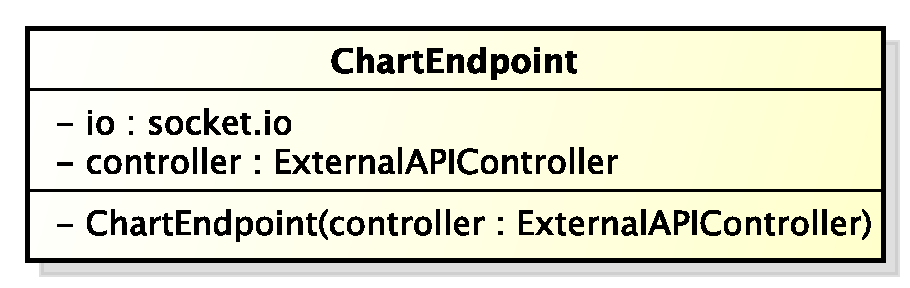
\includegraphics[scale=0.5]{DefinizioneDiProdotto/Pics/Classi/Norris--ExternalAPIManager--ChartEndpoint}
				\caption{Norris::ExternalAPIManager::ChartEndpoint}
			\end{figure}
		}
	
			
			\begin{itemize}
			\item \textbf{Nome:} ChartEndpoint
			\item \textbf{Tipo:} classe
			
		\item \textbf{Astratta:}
		no
			\item \textbf{Visibilità:} package
			\item \textbf{Descrizione:} Questa classe si occupa di gestire le richieste di  grafici da parte dei client, nonchè l'invio degli aggiornamenti dei grafici stessi. In particolare, ad ogni richiesta di un grafico controlla se il client è autenticato all'istanza di Norris. Essa contiene un oggetto del modulo socket.io di Node.js per gestire l'invio dei grafici e degli aggiornamenti tramite canale websocket.
			\item \textbf{Attributi:}
				\begin{itemize}
				\setlength{\itemsep}{5pt}
				
					\item[\ding{111}] {--io : socket.io} \\ [1mm] Questo attributo è un riferimento ad un'istanza di socket.io, utilizzata per fornire le funzionalità.
					\item[\ding{111}] {--controller : ExternalAPIController} \\ [1mm] Questo attributo è un riferimento all'oggetto che permette di ricavare informazioni sull'istanza di Norris.
				\end{itemize}
		
			\item \textbf{Metodi:}
				\begin{itemize}
				\setlength{\itemsep}{5pt}
				
					\item[\ding{111}] {{--ChartEndpoint(controller : ExternalAPIController)}} \\ [1mm] Questo metodo è il costruttore della classe.
				\end{itemize}
		
			\end{itemize}

			
			\level{5}[ChartEndpointFactory]{Norris::ExternalAPIManager::ChartEndpoint::ChartEndpointFactory}
			

		\IfFileExists{DefinizioneDiProdotto/Pics/Classi/Norris--ExternalAPIManager--ChartEndpoint--ChartEndpointFactory.pdf}{
			\begin{figure}[H]
				\centering
				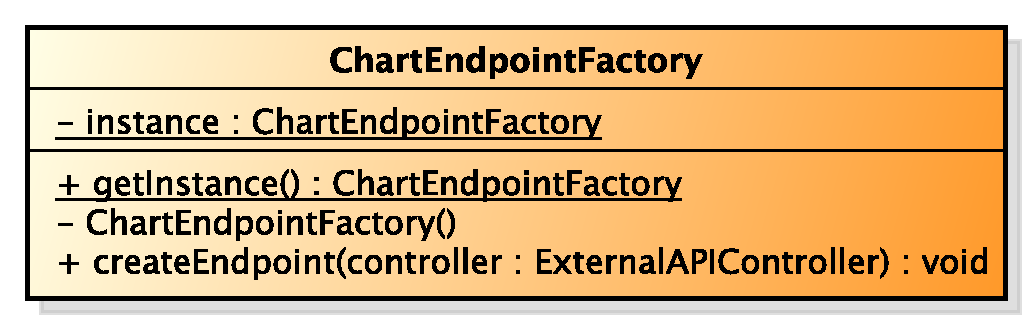
\includegraphics[scale=0.5]{DefinizioneDiProdotto/Pics/Classi/Norris--ExternalAPIManager--ChartEndpoint--ChartEndpointFactory}
				\caption{Norris::ExternalAPIManager::ChartEndpoint::ChartEndpointFactory}
			\end{figure}
		}
	
			
			\begin{itemize}
			\item \textbf{Nome:} ChartEndpointFactory
			\item \textbf{Tipo:} classe
			
		\item \textbf{Astratta:}
		no
			\item \textbf{Visibilità:} private
			\item \textbf{Descrizione:} Questa classe si occupa della creazione di un endpoint di tipo ChartEndpoint.  Tale classe dispone di un blocco di inizializzazione statica che registra la sua istanza nell'array endpoints della classe ExternalAPIConstructor non appena tale classe viene caricata.
			\item \textbf{Attributi:}
				\begin{itemize}
				\setlength{\itemsep}{5pt}
				
					\item[\ding{111}] \underline{--instance : ChartEndpointFactory} \\ [1mm] Questo attributo è il riferimento all'unica istanza della classe.
				\end{itemize}
		
			\item \textbf{Metodi:}
				\begin{itemize}
				\setlength{\itemsep}{5pt}
				
					\item[\ding{111}] {\underline{+getInstance() : ChartEndpointFactory}} \\ [1mm] Questo metodo permette di ottenere l'unica istanza esistente della classe.
					\item[\ding{111}] {{--ChartEndpointFactory()}} \\ [1mm] Questo metodo è il costruttore della classe. Esso è privato perchè non si vuole permettere a nessuno di poter creare un’istanza se non utilizzando il metodo getInstance().

					\item[\ding{111}] {{+createEndpoint(controller : ExternalAPIController) : void}} \\ [1mm] Questo metodo crea un'istanza della classe ChartEndpoint.
				\end{itemize}
		
			\end{itemize}

			
			\level{5}[ChartRef]{Norris::ExternalAPIManager::ChartRef}
			

		\IfFileExists{DefinizioneDiProdotto/Pics/Classi/Norris--ExternalAPIManager--ChartRef.pdf}{
			\begin{figure}[H]
				\centering
				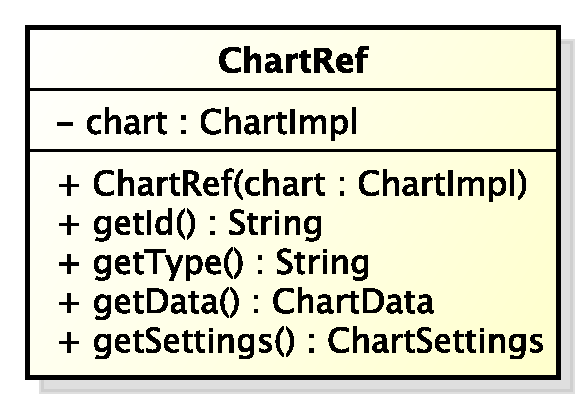
\includegraphics[scale=0.5]{DefinizioneDiProdotto/Pics/Classi/Norris--ExternalAPIManager--ChartRef}
				\caption{Norris::ExternalAPIManager::ChartRef}
			\end{figure}
		}
	
			
			\begin{itemize}
			\item \textbf{Nome:} ChartRef
			\item \textbf{Tipo:} classe
			
		\item \textbf{Estende:}
		EventEmitter
		\item \textbf{Astratta:}
		no
			\item \textbf{Visibilità:} package
			\item \textbf{Descrizione:} Questa classe contiene un riferimento ad un oggetto di tipo ChartModel. È presente un'istanza di ChartRef per ognuno dei grafici dell'istanza di Norris che sono stati richiesti tramite API esterne.
			\item \textbf{Attributi:}
				\begin{itemize}
				\setlength{\itemsep}{5pt}
				
					\item[\ding{111}] {--chart : ChartImpl} \\ [1mm] Questo attributo è un riferimento al chart di Norris rappresentato.
				\end{itemize}
		
			\item \textbf{Metodi:}
				\begin{itemize}
				\setlength{\itemsep}{5pt}
				
					\item[\ding{111}] {{+ChartRef(chart : ChartImpl)}}
					\item[\ding{111}] {{+getId() : String}} \\ [1mm] Questo metodo è il costruttore della classe. Esso dovrà reperire tale informazione dal modello dei dati sfruttando l'attributo privato chart.
					\item[\ding{111}] {{+getType() : String}} \\ [1mm] Questo metodo permette di ottenere il tipo del grafico rappresento. Esso dovrà reperire tale informazione dal modello dei dati sfruttando l'attributo privato chart.
					\item[\ding{111}] {{+getData() : ChartData}} \\ [1mm] Questo metodo permette di ottenere i dati del grafico rappresentato. Esso dovrà reperire tale informazione dal modello dei dati sfruttando l'attributo privato chart.
					\item[\ding{111}] {{+getSettings() : ChartSettings}} \\ [1mm] Questo metodo permette di ottenere le opzioni del grafico rappresentato. Esso dovrà reperire tale informazione dal modello dei dati sfruttando l'attributo privato chart.
				\end{itemize}
		
			\end{itemize}

			
			\level{5}[ExternalAPIConstructor]{Norris::ExternalAPIManager::ExternalAPIConstructor}
			

		\IfFileExists{DefinizioneDiProdotto/Pics/Classi/Norris--ExternalAPIManager--ExternalAPIConstructor.pdf}{
			\begin{figure}[H]
				\centering
				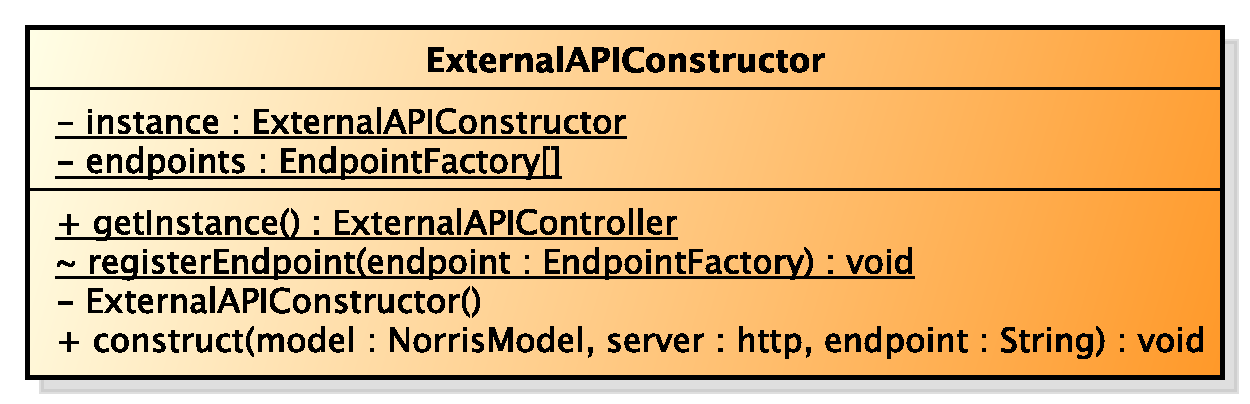
\includegraphics[scale=0.5]{DefinizioneDiProdotto/Pics/Classi/Norris--ExternalAPIManager--ExternalAPIConstructor}
				\caption{Norris::ExternalAPIManager::ExternalAPIConstructor}
			\end{figure}
		}
	
			
			\begin{itemize}
			\item \textbf{Nome:} ExternalAPIConstructor
			\item \textbf{Tipo:} classe
			
		\item \textbf{Astratta:}
		no
			\item \textbf{Visibilità:} public
			\item \textbf{Descrizione:} Questa classe ha la funzione di costruire la componente ExternalAPIManager. Dopo aver creato un'istanza di ExternalAPIController, viene creato un endpoint per ogni dipendenza salvata nell'attributo endpoints.
			\item \textbf{Attributi:}
				\begin{itemize}
				\setlength{\itemsep}{5pt}
				
					\item[\ding{111}] \underline{--instance : ExternalAPIConstructor} \\ [1mm] Questo attributo è il riferimento all'unica istanza della classe.
					\item[\ding{111}] \underline{--endpoints : EndpointFactory[]} \\ [1mm] Questo attributo contiene le dipendenze necessarie per costruire gli endpoint.
				\end{itemize}
		
			\item \textbf{Metodi:}
				\begin{itemize}
				\setlength{\itemsep}{5pt}
				
					\item[\ding{111}] {\underline{+getInstance() : ExternalAPIConstructor}} \\ [1mm] Questo metodo permette di ottenere l'unica istanza esistente della classe.
					\item[\ding{111}] {\underline{\(\sim\)registerEndpoint(endpoint : EndpointFactory) : void}} \\ [1mm] Questo metodo permette di registrare le dipendenze per la creazione di nuovi endpoint. Tale metodo permette alle factory di registrarsi nel vettore delle factory (endpoints) permettendone così l'utilizzo.
					\item[\ding{111}] {{--ExternalAPIConstructor()}} \\ [1mm] Questo metodo è il costruttore della classe.  Esso è privato perchè non si vuole permettere a nessuno di poter creare un’istanza se non utilizzando il metodo getInstance().

					\item[\ding{111}] {{+construct(model : NorrisImpl, server : http, app : express) : void}} \\ [1mm] Questo metodo permette di costruire la componente ExternalAPIManager in funzione dei parametri passati.
				\end{itemize}
		
			\end{itemize}

			
			\level{5}[ExternalAPIController]{Norris::ExternalAPIManager::ExternalAPIController}
			

		\IfFileExists{DefinizioneDiProdotto/Pics/Classi/Norris--ExternalAPIManager--ExternalAPIController.pdf}{
			\begin{figure}[H]
				\centering
				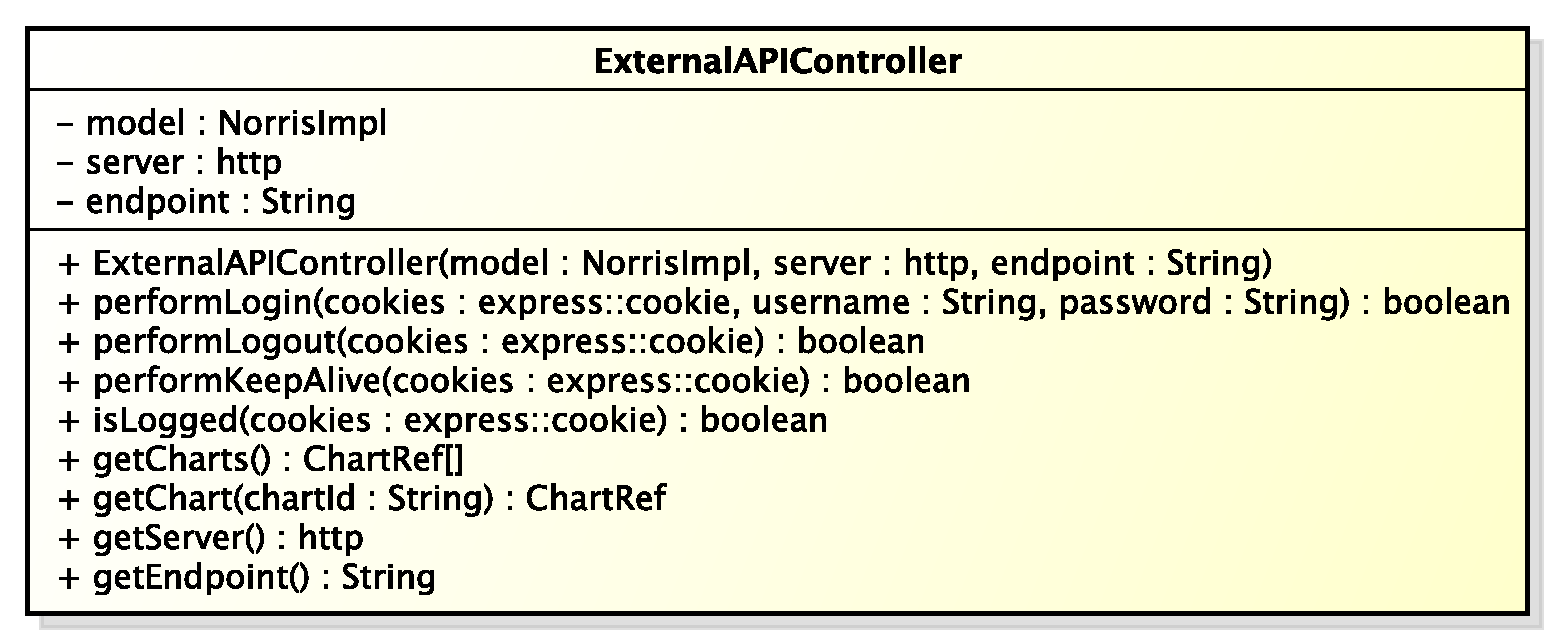
\includegraphics[scale=0.5]{DefinizioneDiProdotto/Pics/Classi/Norris--ExternalAPIManager--ExternalAPIController}
				\caption{Norris::ExternalAPIManager::ExternalAPIController}
			\end{figure}
		}
	
			
			\begin{itemize}
			\item \textbf{Nome:} ExternalAPIController
			\item \textbf{Tipo:} classe
			
		\item \textbf{Estende:}
		EventEmitter
		\item \textbf{Astratta:}
		no
			\item \textbf{Visibilità:} package
			\item \textbf{Descrizione:} Al suo interno ci sono un riferimento al NorrisModel ed un riferimento ad un oggetto del modulo http di Node.js. Contiene inoltre l'interfaccia EndPointFactory.
			\item \textbf{Attributi:}
				\begin{itemize}
				\setlength{\itemsep}{5pt}
				
					\item[\ding{111}] {--model : NorrisImpl} \\ [1mm] Questo attributo è un riferimento al modello di Norris sul quale si basa la componente ExternalAPIManager.
					\item[\ding{111}] {--server : http} \\ [1mm] Questo attributo è l'istanza del webserver che la componente utilizza per offrire le sue funzionalità.
					\item[\ding{111}] {--app : express}
				\end{itemize}
		
			\item \textbf{Metodi:}
				\begin{itemize}
				\setlength{\itemsep}{5pt}
				
					\item[\ding{111}] {{+ExternalAPIController(model : NorrisImpl, server : http, app : express)}} \\ [1mm] Questo metodo è il costruttore della classe.
					\item[\ding{111}] {{+performLogin(cookies : express::cookie, username : String, password : String) : boolean}} \\ [1mm] Questo metodo avvia una nuova sessione per l'utente e permette di impostare il token tramite il parametro cookies. 
					\item[\ding{111}] {{+performLogout(cookies : express::cookie) : boolean}} \\ [1mm] Questo metodo permette di terminare la sessione di un utente mediante i cookie passati come parametro.
					\item[\ding{111}] {{+performKeepAlive(cookies : express::cookie) : boolean}} \\ [1mm] Questo metodo permette di rinnovare la sessione di un utente mediante i cookie passati come parametro.
					\item[\ding{111}] {{+isLogged(cookies : express::cookie) : boolean}} \\ [1mm] Questo metodo permette di verificare se l'utente è autenticato tramite i cookie passati come parametro.
					\item[\ding{111}] {{+getCharts() : ChartRef[]}} \\ [1mm] Questo metodo permette di ottenere una lista di tutti i grafici presenti nell'istanza di Norris rappresentata.
					\item[\ding{111}] {{+getChart(chartId : String) : ChartRef}} \\ [1mm] Questo metodo permette di ottenere un chart contenuto nell'istanza di Norris rappresentata tramite il suo id.
					\item[\ding{111}] {{+getServer() : http}} \\ [1mm] Questo metodo permette di ottenere il server.
					\item[\ding{111}] {{+getEndpoint() : String}} \\ [1mm] Questo metodo permette di ottenere l'endpoint sul quale sono fornite le API.
					\item[\ding{111}] {{+getApp() : express}}
				\end{itemize}
		
			\end{itemize}

			
			\level{5}[ListEndpoint]{Norris::ExternalAPIManager::ListEndpoint}
			

		\IfFileExists{DefinizioneDiProdotto/Pics/Classi/Norris--ExternalAPIManager--ListEndpoint.pdf}{
			\begin{figure}[H]
				\centering
				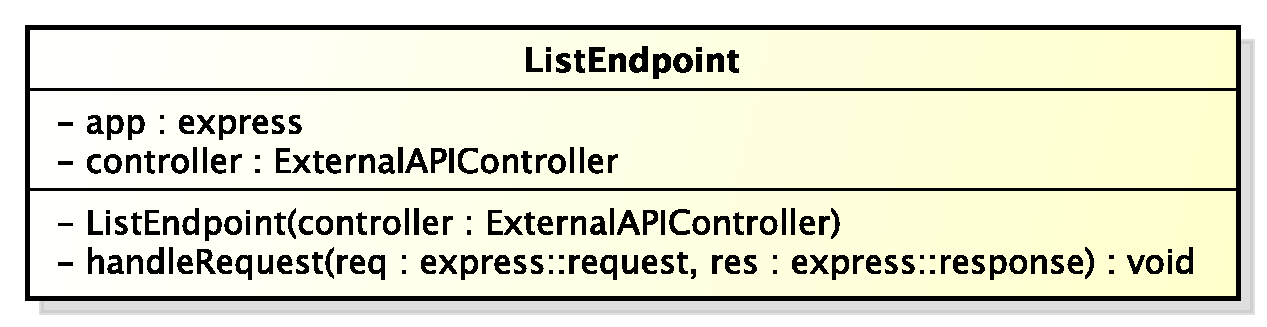
\includegraphics[scale=0.5]{DefinizioneDiProdotto/Pics/Classi/Norris--ExternalAPIManager--ListEndpoint}
				\caption{Norris::ExternalAPIManager::ListEndpoint}
			\end{figure}
		}
	
			
			\begin{itemize}
			\item \textbf{Nome:} ListEndpoint
			\item \textbf{Tipo:} classe
			
		\item \textbf{Astratta:}
		no
			\item \textbf{Visibilità:} package
			\item \textbf{Descrizione:} Questa classe si occupa di gestire le richieste della lista dei  grafici da parte dei client. In particolare, ad ogni richiesta della lista controlla se il client è autenticato all'istanza di Norris. Essa contiene un oggetto del modulo express di Node.js per gestire l'invio della lista di grafici tramite richiesta HTTP.
			\item \textbf{Attributi:}
				\begin{itemize}
				\setlength{\itemsep}{5pt}
				
					\item[\ding{111}] {--controller : ExternalAPIController} \\ [1mm] Questo attributo è un riferimento all'oggetto che permette di ricavare informazioni sull'istanza di Norris.
				\end{itemize}
		
			\item \textbf{Metodi:}
				\begin{itemize}
				\setlength{\itemsep}{5pt}
				
					\item[\ding{111}] {{--ListEndpoint(controller : ExternalAPIController)}} \\ [1mm] Questo metodo è il costruttore della classe.
					\item[\ding{111}] {{--handleRequest(req : express::request, res : express::response) : void}} \\ [1mm] Questo metodo gestisce una richiesta per l'ottenimento della lista dei grafici.
				\end{itemize}
		
			\end{itemize}

			
			\level{5}[ListEndpointFactory]{Norris::ExternalAPIManager::ListEndpoint::ListEndpointFactory}
			

		\IfFileExists{DefinizioneDiProdotto/Pics/Classi/Norris--ExternalAPIManager--ListEndpoint--ListEndpointFactory.pdf}{
			\begin{figure}[H]
				\centering
				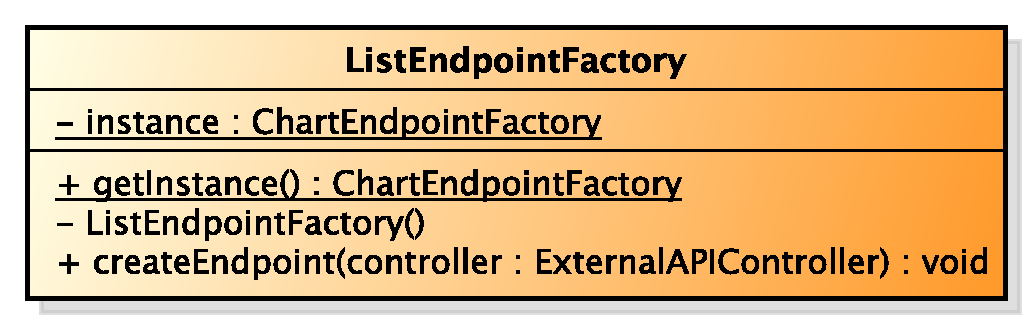
\includegraphics[scale=0.5]{DefinizioneDiProdotto/Pics/Classi/Norris--ExternalAPIManager--ListEndpoint--ListEndpointFactory}
				\caption{Norris::ExternalAPIManager::ListEndpoint::ListEndpointFactory}
			\end{figure}
		}
	
			
			\begin{itemize}
			\item \textbf{Nome:} ListEndpointFactory
			\item \textbf{Tipo:} classe
			
		\item \textbf{Astratta:}
		no
			\item \textbf{Visibilità:} private
			\item \textbf{Descrizione:} Questa classe si occupa della creazione di un endpoint di tipo ListEndpoint. Tale classe dispone di un blocco di inizializzazione statica che registra la sua istanza nell'array endpoints della classe ExternalAPIConstructor non appena tale classe viene caricata.
			\item \textbf{Attributi:}
				\begin{itemize}
				\setlength{\itemsep}{5pt}
				
					\item[\ding{111}] \underline{--instance : ChartEndpointFactory} \\ [1mm] Questo attributo è il riferimento all'unica istanza della classe.
				\end{itemize}
		
			\item \textbf{Metodi:}
				\begin{itemize}
				\setlength{\itemsep}{5pt}
				
					\item[\ding{111}] {\underline{+getInstance() : ChartEndpointFactory}} \\ [1mm] Questo metodo permette di ottenere l'unica istanza esistente della classe.
					\item[\ding{111}] {{--ListEndpointFactory()}} \\ [1mm] Questo metodo è il costruttore della classe. Esso è privato perchè non si vuole permettere a nessuno di poter creare un’istanza se non utilizzando il metodo getInstance().

					\item[\ding{111}] {{+createEndpoint(controller : ExternalAPIController) : void}} \\ [1mm] Questo metodo crea un'istanza della classe ListtEndpoint.
				\end{itemize}
		
			\end{itemize}

			
	\level{1}{Chuck}
    \level{2}{Specifica dei componenti}
        Nella presente sezione è stata riportata e documentata la progettazione di dettaglio del \insglo{prodotto} \insglo{Chuck}. Si noti che tale progettazione deriva direttamente dalla progettazione architetturale che può essere trovata all'interno del documento \insdoc{Specifica Tecnica v5.00}. I risultati ottenuti sono stati organizzati e presentati secondo la seguente struttura:
        \begin{enumerate}
            \item vengono innanzitutto presentate le varie classi che sono state individuate. Per ognuna di esse si indica il nome, il tipo, l'eventuale astrattezza, la visibilità e il fatto che estenda altre classi oppure no. In aggiunta a ciò, viene presentata una descrizione completa del ruolo e delle responsabilità della classe oltre a una documentazione completa riguardante tutti gli attributi e i metodi presenti all'interno.
            \item in secondo luogo vengono presentati i diagrammi di sequenza, che hanno lo scopo di descrivere scenari (determinate sequenze di azioni in cui tutte le scelte sono già state effettuate). Essi vengono usati per descrivere le relazioni che intercorrono, in termini di messaggi, tra attori, oggetti ed entità del sistema \insglo{Chuck}.
        \end{enumerate}
        Le regole che sono state rispettate, gli strumenti che sono stati usati e le procedure che sono state effettuate possono essere trovate all'interno del documento \insdoc{Norme di Progetto v6.00}.
        \level{3}{Gerarchie presenti in Chuck}
            Di seguito vengono elencate tutte le gerarchie presenti in \insglo{Chuck} per fornire in forma visiva tutti i tipi implementati/estesi dalle singole componenti.
            \begin{itemize}
                \item Gerarchie in Model::NorrisChart \\
                    La seguente gerarchia rappresenta tutte le tipologie di chart utilizzate in \insglo{Chuck}.
                    \begin{figure}[H]
                        \centering
                        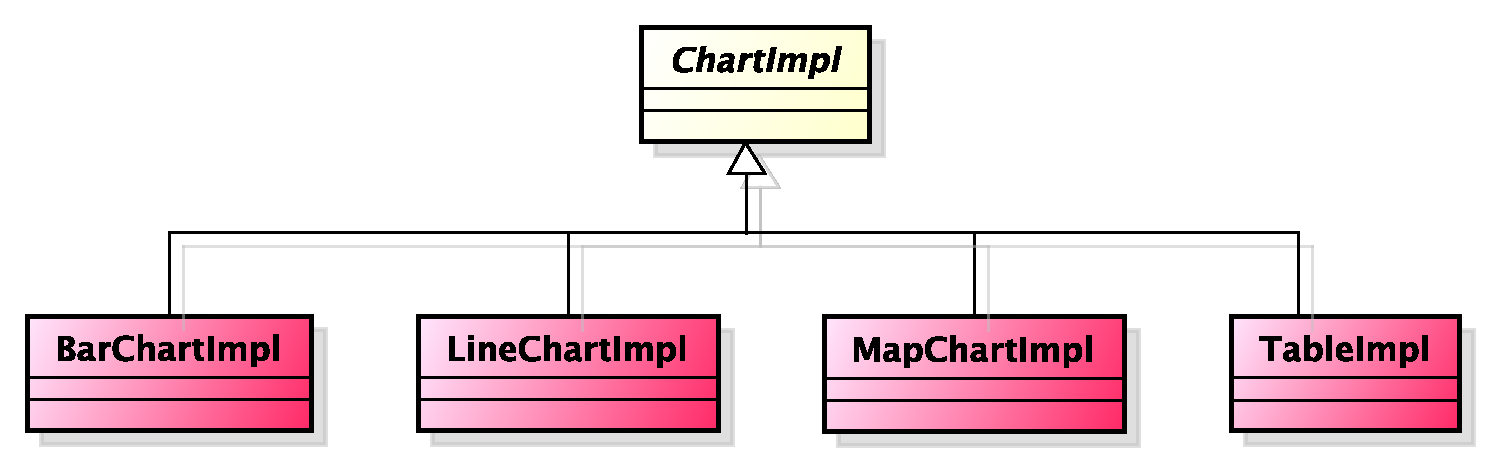
\includegraphics[width=1\textwidth]{DefinizioneDiProdotto/Pics/Gerarchie/ModelChartImpl.pdf}
                        \caption{Diagramma gerarchia ChartImpl in Chuck Model::NorrisChart }
                    \end{figure}
                    La seguente gerarchia rappresenta tutte le tipologie di chart factory che permettono la creazione dei vari chart.
                    \begin{figure}[H]
                        \centering
                        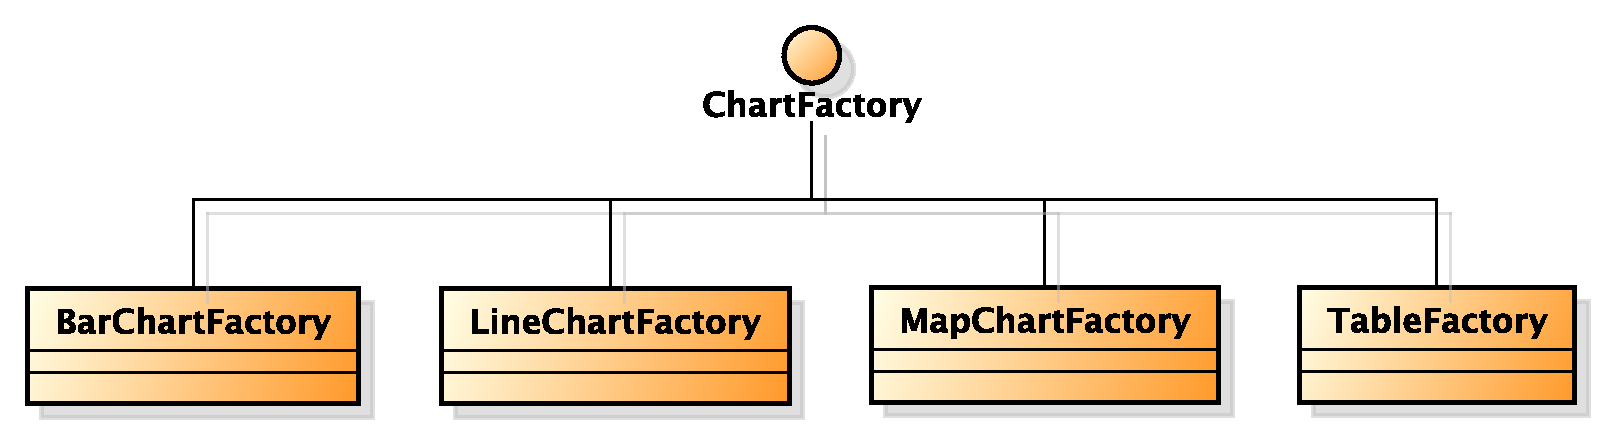
\includegraphics[width=1\textwidth]{DefinizioneDiProdotto/Pics/Gerarchie/ModelFactory.pdf}
                        \caption{Diagramma gerarchia ChartFactory in Chuck Model::NorrisChart}
                    \end{figure}
                    La seguente gerarchia rappresenta tutte le tipologie di updater che possono esser utilizzate per aggiornare un chart.
                    \begin{figure}[H]
                        \centering
                        \includegraphics[width=1\textwidth]{DefinizioneDiProdotto/Pics/Gerarchie/ModelUpdater.pdf}
                        \caption{Diagramma gerarchia Updater in Chuck Model::NorrisChart }
                    \end{figure}
                \item Gerarchie in Model::Services \\
                    La seguente gerarchia rappresenta i servizi utilizzati in \insglo{Chuck}.
                    \begin{figure}[H]
                        \centering
                        \includegraphics[width=1\textwidth]{DefinizioneDiProdotto/Pics/Gerarchie/ChuckService.pdf}
                        \caption{Diagramma gerarchia dei services in Chuck Model::Services}
                    \end{figure}
                \item Gerarchie in ViewModel \\
                    La seguente gerarchia rappresenta tutte le view-model utilizzate in \insglo{Chuck}.
                    \begin{figure}[H]
                        \centering
                        \includegraphics[width=1\textwidth]{DefinizioneDiProdotto/Pics/Gerarchie/ChuckViewModel.pdf}
                        \caption{Diagramma gerarchia dei view-model in Chuck ViewModel}
                    \end{figure}
                \item Gerarchie in Directive \\
                    La seguente gerarchia rappresenta le varie directive utilizzate in \insglo{Chuck}.
                    \begin{figure}[H]
                        \centering
                        \includegraphics[width=1\textwidth]{DefinizioneDiProdotto/Pics/Gerarchie/ChuckDirective.pdf}
                        \caption{Diagramma gerarchia delle directive in Chuck Directive}
                    \end{figure}
                \item Gerarchie in View \\
                    La seguente gerarchia rappresenta le varie view utilizzate in \insglo{Chuck}.
                    \begin{figure}[H]
                        \centering
                        \includegraphics[width=1\textwidth]{DefinizioneDiProdotto/Pics/Gerarchie/ChuckView.pdf}
                        \caption{Diagramma gerarchia delle view in Chuck View}
                    \end{figure}
            \end{itemize}

        \level{3}{Classi}
            In tale sezione sono riportate delle descrizioni dettagliate delle classi individuate all'interno del documento \insdoc{Specifica Tecnica v4.00}. Tali classi sono presentate e organizzate in modo gerarchico, mantenendo una suddivisione per \insglo{package} di appartenenza.
            \level{1}{Chuck}
    \level{2}{Specifica dei componenti}
        Nella presente sezione è stata riportata e documentata la progettazione di dettaglio del \insglo{prodotto} \insglo{Chuck}. Si noti che tale progettazione deriva direttamente dalla progettazione architetturale che può essere trovata all'interno del documento \insdoc{Specifica Tecnica v5.00}. I risultati ottenuti sono stati organizzati e presentati secondo la seguente struttura:
        \begin{enumerate}
            \item vengono innanzitutto presentate le varie classi che sono state individuate. Per ognuna di esse si indica il nome, il tipo, l'eventuale astrattezza, la visibilità e il fatto che estenda altre classi oppure no. In aggiunta a ciò, viene presentata una descrizione completa del ruolo e delle responsabilità della classe oltre a una documentazione completa riguardante tutti gli attributi e i metodi presenti all'interno.
            \item in secondo luogo vengono presentati i diagrammi di sequenza, che hanno lo scopo di descrivere scenari (determinate sequenze di azioni in cui tutte le scelte sono già state effettuate). Essi vengono usati per descrivere le relazioni che intercorrono, in termini di messaggi, tra attori, oggetti ed entità del sistema \insglo{Chuck}.
        \end{enumerate}
        Le regole che sono state rispettate, gli strumenti che sono stati usati e le procedure che sono state effettuate possono essere trovate all'interno del documento \insdoc{Norme di Progetto v6.00}.
        \level{3}{Gerarchie presenti in Chuck}
            Di seguito vengono elencate tutte le gerarchie presenti in \insglo{Chuck} per fornire in forma visiva tutti i tipi implementati/estesi dalle singole componenti.
            \begin{itemize}
                \item Gerarchie in Model::NorrisChart \\
                    La seguente gerarchia rappresenta tutte le tipologie di chart utilizzate in \insglo{Chuck}.
                    \begin{figure}[H]
                        \centering
                        \includegraphics[width=1\textwidth]{DefinizioneDiProdotto/Pics/Gerarchie/ModelChartImpl.pdf}
                        \caption{Diagramma gerarchia ChartImpl in Chuck Model::NorrisChart }
                    \end{figure}
                    La seguente gerarchia rappresenta tutte le tipologie di chart factory che permettono la creazione dei vari chart.
                    \begin{figure}[H]
                        \centering
                        \includegraphics[width=1\textwidth]{DefinizioneDiProdotto/Pics/Gerarchie/ModelFactory.pdf}
                        \caption{Diagramma gerarchia ChartFactory in Chuck Model::NorrisChart}
                    \end{figure}
                    La seguente gerarchia rappresenta tutte le tipologie di updater che possono esser utilizzate per aggiornare un chart.
                    \begin{figure}[H]
                        \centering
                        \includegraphics[width=1\textwidth]{DefinizioneDiProdotto/Pics/Gerarchie/ModelUpdater.pdf}
                        \caption{Diagramma gerarchia Updater in Chuck Model::NorrisChart }
                    \end{figure}
                \item Gerarchie in Model::Services \\
                    La seguente gerarchia rappresenta i servizi utilizzati in \insglo{Chuck}.
                    \begin{figure}[H]
                        \centering
                        \includegraphics[width=1\textwidth]{DefinizioneDiProdotto/Pics/Gerarchie/ChuckService.pdf}
                        \caption{Diagramma gerarchia dei services in Chuck Model::Services}
                    \end{figure}
                \item Gerarchie in ViewModel \\
                    La seguente gerarchia rappresenta tutte le view-model utilizzate in \insglo{Chuck}.
                    \begin{figure}[H]
                        \centering
                        \includegraphics[width=1\textwidth]{DefinizioneDiProdotto/Pics/Gerarchie/ChuckViewModel.pdf}
                        \caption{Diagramma gerarchia dei view-model in Chuck ViewModel}
                    \end{figure}
                \item Gerarchie in Directive \\
                    La seguente gerarchia rappresenta le varie directive utilizzate in \insglo{Chuck}.
                    \begin{figure}[H]
                        \centering
                        \includegraphics[width=1\textwidth]{DefinizioneDiProdotto/Pics/Gerarchie/ChuckDirective.pdf}
                        \caption{Diagramma gerarchia delle directive in Chuck Directive}
                    \end{figure}
                \item Gerarchie in View \\
                    La seguente gerarchia rappresenta le varie view utilizzate in \insglo{Chuck}.
                    \begin{figure}[H]
                        \centering
                        \includegraphics[width=1\textwidth]{DefinizioneDiProdotto/Pics/Gerarchie/ChuckView.pdf}
                        \caption{Diagramma gerarchia delle view in Chuck View}
                    \end{figure}
            \end{itemize}

        \level{3}{Classi}
            In tale sezione sono riportate delle descrizioni dettagliate delle classi individuate all'interno del documento \insdoc{Specifica Tecnica v4.00}. Tali classi sono presentate e organizzate in modo gerarchico, mantenendo una suddivisione per \insglo{package} di appartenenza.
            \input{Classi/Chuck.tex}

    \level{2}{Diagrammi di sequenza}
        In tale sezione vengono presentati i diagrammi di sequenza, che hanno lo scopo di descrivere scenari (determinate sequenze di azioni in cui tutte le scelte sono già state effettuate). Essi vengono usati per descrivere le relazioni che intercorrono, in termini di messaggi, tra attori, oggetti ed entità del sistema \insglo{Chuck}.
        \level{3}{Creazione di un chart}
             Tale diagramma riporta e descrive come viene creato un chart e collegato a quello presente all'interno di una certa istanza di \insglo{Norris}.
            \begin{figure}[H]
                \centering
                \includegraphics[scale=0.3]{DefinizioneDiProdotto/Pics/ChuckInserimentoChart}
                \caption{Diagramma di sequenza - Chuck, creazione chart}
            \end{figure}
            \begin{enumerate}
                \item ChartViewModel richiede l'ottenimento di un chart specifico presente in una istanza di \insglo{Norris} a ChartRequester;
                \item questo apre il canale socket ed imposta delle \insglo{callback} per gli eventi chart e update;
                \item ricevuto il grafico crea il modello dei dati;
                \item infine ChartViewModel esegue il metodo init che permette di inizializzare la view e visualizzare il Chart secondo i dati memorizzati.
            \end{enumerate}

        \level{3}{Aggiornamento di un chart}
            Tale diagramma descrive come viene aggiornato un chart nel momento in cui arrivano nuovi dati dall'istanza di \insglo{Norris} alla quale il grafico appartiene.
            \begin{figure}[H]
                \centering
                \includegraphics[scale=0.3]{DefinizioneDiProdotto/Pics/ChuckAggiornamentoChart}
                \caption{Diagramma di sequenza - Chuck, aggiornamento chart}
            \end{figure}
            \begin{enumerate}
                \item il messaggio iniziale rappresenta la notifica inviata da ChartRequester da parte di \insglo{Norris} attraverso il canale socket per avvertirlo dell'avvenuto aggiornamento;
                \item ChartRequester aggiorna il modello dei dati;
                \item avverte infine il ChartViewModel di un'avvenuta modifica nel modello richiedendo dunque la renderizzazione dei nuovi dati.
                \item
                \item
                \item
            \end{enumerate}


    \level{2}{Diagrammi di sequenza}
        In tale sezione vengono presentati i diagrammi di sequenza, che hanno lo scopo di descrivere scenari (determinate sequenze di azioni in cui tutte le scelte sono già state effettuate). Essi vengono usati per descrivere le relazioni che intercorrono, in termini di messaggi, tra attori, oggetti ed entità del sistema \insglo{Chuck}.
        \level{3}{Creazione di un chart}
             Tale diagramma riporta e descrive come viene creato un chart e collegato a quello presente all'interno di una certa istanza di \insglo{Norris}.
            \begin{figure}[H]
                \centering
                \includegraphics[scale=0.3]{DefinizioneDiProdotto/Pics/ChuckInserimentoChart}
                \caption{Diagramma di sequenza - Chuck, creazione chart}
            \end{figure}
            \begin{enumerate}
                \item ChartViewModel richiede l'ottenimento di un chart specifico presente in una istanza di \insglo{Norris} a ChartRequester;
                \item questo apre il canale socket ed imposta delle \insglo{callback} per gli eventi chart e update;
                \item ricevuto il grafico crea il modello dei dati;
                \item infine ChartViewModel esegue il metodo init che permette di inizializzare la view e visualizzare il Chart secondo i dati memorizzati.
            \end{enumerate}

        \level{3}{Aggiornamento di un chart}
            Tale diagramma descrive come viene aggiornato un chart nel momento in cui arrivano nuovi dati dall'istanza di \insglo{Norris} alla quale il grafico appartiene.
            \begin{figure}[H]
                \centering
                \includegraphics[scale=0.3]{DefinizioneDiProdotto/Pics/ChuckAggiornamentoChart}
                \caption{Diagramma di sequenza - Chuck, aggiornamento chart}
            \end{figure}
            \begin{enumerate}
                \item il messaggio iniziale rappresenta la notifica inviata da ChartRequester da parte di \insglo{Norris} attraverso il canale socket per avvertirlo dell'avvenuto aggiornamento;
                \item ChartRequester aggiorna il modello dei dati;
                \item avverte infine il ChartViewModel di un'avvenuta modifica nel modello richiedendo dunque la renderizzazione dei nuovi dati.
                \item
                \item
                \item
            \end{enumerate}

	\level{2}{Applicazione Android}
    Il diagramma sottostante rappresenta la vista ad alto livello dell'applicazione Android.
   
    \begin{figure}[H]\centering
        \includegraphics[width=\textwidth]{SpecificaTecnica/Pics/AndroidAppComponentDiagramLevel0.png}
        \caption{Diagramma delle componenti App Android}
    \end{figure}

    \level{3}{Descrizione delle componenti principali della app}
    	\level{4}{Model} 
        Il Model è la componente che rappresenta l'astrazione dei grafici visualizzati nell'applicazione. In essa sono contenuti i dati riguardanti i grafici, assieme alle relative impostazioni. In particolare sono presenti i modelli di tutte le tipologie di chart implementati da Norris. Il Data Model fornisce per ciascuna tipologia di grafico i metodi per inserire i dati e configurare alcune impostazioni. 
    
       \level{4}{View}
        La View è il componente che rappresenta le varie UI dell'applicazione e i vari widget dei grafici da inserire nelle UI. In tale componente potrebbero esser sollevati degli eventi scatenati dall'utente.
       \level{4}{Controller}
        Questo componente ha il compito di gestire tutto il controllo dell'applicazione. Le operazioni che esso gestisce sono riassunte nel seguente elenco:
        	\begin{itemize}
        		\item creazione del modello qualora questo sia necessario;
        		\item utilizzo delle API esterne di Norris;
        		\item interpretazione dei pacchetti ricevuti dal server contenenti i dati delle richieste API;
        		\item ascolto sul canale socket per ricevere gli aggiornamenti di stato dei chart;
        		\item interpretazione dei pacchetti di aggiornamento;
        		\item richiesta al modello di aggiornare il proprio stato;
        		\item richiesta della creazione dei widget dei grafici da inserire nelle UI dell'applicazioe;
        		\item avvio delle varie activity dell'applicazione;
        		\item gestione delle gesture dell'utente.
        \end{itemize}
    \level{2}{Descrizione delle interazioni che i componenti dell'app hanno tra di loro}
    	Le interazioni tra i componenti sono rappresentati con una freccia. Sono presenti due tipologie di frecce:
    	\begin{itemize}
    			\item{continua: } rappresenta l'invocazione di un metodo;
    			\item{tratteggiata: } rappresenta lo scatenarsi di un evento.
    		\end{itemize}
    	Riportiamo di seguito la descrizione di ogni interazione.
    	\level{4}{User Gesture}
	    La freccia etichettata con il termine "User Gesture" rappresenta l'interazione tra View e Controller. In seguito all'esecuzione di una gesture da parte dell'utente, la View notifica il Controller tramite l'emissione di un evento opportuno. Il Controller si occupa quindi di gestire tale evento. Questa interazione si verifica in particolare quando l'utente seleziona un item della lista dei grafici presenti nell'istanza di Norris richiesta.
	    \level{4}{API Request}
	    La freccia etichettata con il termine "API Request" rappresenta l'interazione tra il Controller e le API esterne di Norris. Il Controller richiama le API esterne per connettersi ad un'istaza di Norris, per richiedere la lista di grafici presenti presso quell'istanza e per ottenere le informazioni sui singoli grafici. Le API esterne rispondono al Controller con l'invio dei dati richiesti solo se l'autenticazione è andata a buon fine. Per la spiegazione in dettaglio delle funzionalità offerte dalle API esterne, si rimanda al documento \insdoc{Analisi dei Requisiti v.X.xx}.
	    \level{4}{Update Notification}
	   	La freccia etichettata con il termine "Update Notification" rappresenta l'interazione tra le API esterne di Norris e il Controller. Le API esterne notificano il Controller che è stato aggiornato il modello di un grafico nel Server. Tramite il canale socket viene inviato l'aggiornamento avvenuto e l'id del grafico che è stato aggiornato, in modo che il Controller possa occuparsi della gestione dell'aggiornamento nell'applicazione.
	    	
	    \level{4}{State Change}
	    La freccia etichettata con il termine "State Change" rappresenta l'interazione tra il Controller e il Model. Il Controller richiede al Model di modificare il proprio stato in seguito alla richiesta di un nuovo grafico o in seguito all'aggiornamento di un grafico già presente.
	    \level{4}{Change Notification}
	   	La freccia etichettata con il termine "Change Notification" rappresenta l'interazione tra il Model e la View. Il Model notifica le View che lo osservano ogniqualvolta il suo stato viene modificato. Le View dovranno quindi modificare a loro volta il proprio stato, in modo da essere sempre coerenti col modello.
	    \level{4}{State Query}
	   	La freccia etichettata con il termine "State Query" rappresenta l'interazione tra la View e il Model. Questa interazione rappresenta la richiesta dello stato del Model da parte della View. Viene effettuata quando la View ha la necessità di esporre i dati del Model o qualcosa che sia dipendente dallo stato di quest'ultimo. Ciò si verifica quando si deve mostrare un nuovo grafico o quando si devono mostrare gli aggiornamenti di un grafico già presente.
	    \level{4}{View Selection}
	   	La freccia etichettata con il termine "View Selection" rappresenta l'interazione tra il Controller e la View. Tale interazione rappresenta la richiesta da parte del Controller di visualizzare una specifica Activity.


	\level{1}{Dashboard}
    Nel documento \insdoc{Specifica Tecnica v4.00} è stato definito in modo generale quali sono i componenti di cui è composta la Dashboard e ne sono stati definiti in modo preciso i ruoli. In esso, inoltre, è stato descritto il modo in cui l'utilizzatore di Norris deve procedere per creare e rendere disponibile la Dashboard.\\
    I task che lo sviluppatore deve eseguire durante la creazione della Dashboard sono talvolta complessi, nel senso che alcuni di essi implicano operazioni ulteriori rispetto al semplice uso dell API interne fornite da Norris. Si è dunque deciso di suddividere l'intera logica di creazione e aggiornamento dei grafici e della pagina che andranno a formare la Dashboard in diverse funzioni. È stato fatto questo perchè in tale modo il codice è più modulare e comprensibile.
    \level{2}{Funzioni}
        Nel presente paragrafo vengono presentate le funzioni nelle quali è stato suddiviso il codice necessario alla creazione e all'aggiornamento della Dashboard. Tali funzioni, si ricordi, fanno riferimento ai task che sono stati presentati e descritti nel documento \insdoc{Specifica Tecnica v4.00}.\\
        Si noti che le funzioni qui presentate rappresentano solo una ulteriore semplificazione fornita agli sviluppatori per creare una Dashboard basata sui dati messi a disposizione dall'APS. Nessuno vieta loro, infatti, di utilizzare in modo base le API interne che sono messe a disposizione da Norris e che sono descritte e documentate all'interno del presente documento.\\
        All'appendice \nameref{app:aps} si possono trovare le specifiche con le quali vengono effettuate le richieste al server APS. In tale appendice è riportato anche il formato della risposta che si ottiene, oltre ai criteri per interpretarlo.

        \begin{description}

            \item \textbf{init\_norris() : Norris} \\
            Tale funzione ha il compito di inizializzare l'istanza di Norris. Ciò fa si che nel webserver si crei l'istanza vera e propria e ne vengano settate le impostazioni. Ne viene infine montato il middleware con express e ritornato.
            
            \item \textbf{init\_map(norris : Norris) : Chart} \\
            Tale funzione ha il compito di inizializzare un map chart nell'istanza di Norris. Il chart non conterrà dati (che saranno inseriti in seguito, tramite aggiornamenti). Vengono inoltre impostate alcune opzioni di default. Il map chart che è stato creato da tale funzione viene ritornato, in modo che sia utilizzabile dallo sviluppatore in modo autonomo.
            
            \item \textbf{init\_bar(norris : Norris) : Chart} \\
            Tale funzione ha il compito di inizializzare un bar chart nell'istanza di Norris. Il chart non conterrà dati (che saranno inseriti in seguito, tramite aggiornamenti). Vengono inoltre impostate alcune opzioni di default. Il bar chart che è stato creato da tale funzione viene ritornato, in modo che sia utilizzabile dallo sviluppatore in modo autonomo.
            
            \item \textbf{init\_table(norris : Norris) : Chart} \\
            Tale funzione ha il compito di inizializzare una table nell'istanza di Norris. Il chart viene inizializzato con dati riguardanti alcuni dei principali punti di interesse di Padova (Prato della Valle, Stazione FS, Ospedale Civile), che però sono impostati su "unknown". Essi saranno correttamente aggiornati in un momento successivo, quando vengono ricevuti i dati dal server APS.
            
            \item \textbf{init\_page(norris : Norris, charts : Chart[]) : Page} \\
            Tale funzione ha il compito di inizializzare una pagina in una certa istanza di Norris. La pagina viene creata a partire dai grafici che sono stati passati come parametro alla funzione, e che presumibilmente (ma non obbligatoriamente) sono quelli ottenuti a partire dalle funzioni presentate in precedenza. Tale funzione si occupa inoltre di impostare alcune opzioni di default per la pagina.
            
            \item \textbf{getLines() : Dataset[]} \\
            Tale funzione ha il compito di ottenere tutti i dati riguardanti le linee che il server APS mette a disposizione. Si noti che i dati che vengono ritornati sono nel formato fornito dall'APS, e quindi devono essere correttamente interpretati e convertiti prima di essere usati tramite le API di Norris. Il formato con il quale sono restituiti i dati da tale funzione sono descritti nell'appendice \nameref{app:aps}.
            
            \item \textbf{update\_map(chart : Chart, old\_values : Dataset[], new\_values : Dataset[]) : void} \\
            Tale funzione ha il compito di aggiornare il map chart a partire dai dati che sono stati passati come parametro alla funzione. Tali dati sono quelli che sono stati ritornati dalla funzione getLines: essi sono dunque prima di tutto convertiti in un formato fruibile da Norris. In seguito, questi dati vengono utilizzati tramite le API interne per aggiornare il map chart: vengono aggiornate le posizioni di tutti i punti sulla mappa, vengono aggiunti eventuali nuovi punti e vengono tolti quelli non più presenti.
            
            \item \textbf{update\_bar(chart : Chart, old\_values : Dataset[], new\_values : Dataset[]) : void} \\
            Tale funzione ha il compito di aggiornare il bar chart a partire dai dati che sono stati passati come parametro alla funzione. Tali dati sono quelli che sono stati ritornati dalla funzione getLines: essi devono dunque subire un'elaborazione, in quanto il bar chart deve contenere un'aggregazione dei dati che sono stati ottenuti, e non ogni singolo dato. In particolare, tale funzione si occupa di calcolare quanti mezzi sono attivi per ciascuna linea. A partire poi dal risultato ottenuto viene creato il pacchetto di aggiornamento tramite il quale le API interne possono effettuare l'aggiornamento vero e proprio del grafico.
            
            \item \textbf{update\_table(chart : Chart, old\_values : Dataset[], new\_values : Dataset[]) : void} \\
            Tale funzione ha il compito di aggiornare la table a partire dai dati che sono stati passati come parametro alla funzione. Tali dati sono quelli che sono stati ritornati dalla funzione getLines: essi devono dunque subire un'elaborazione, in quanto la table deve contenere un'aggregazione dei dati che sono stati ottenuti, e non ogni singolo dato. In particolare, tale funzione si occupa di calcolare qual'è il mezzo più vicino ai vari punti di interesse e qual'è il tempo di attesa medio. A partire poi dal risultato ottenuto viene creato il pacchetto di aggiornamento tramite il quale le API interne possono effettuare l'aggiornamento vero e proprio del grafico.

        \end{description}
	
		\newpage
		\level{1}{Stime di fattibilità e di bisogno di risorse}
Dopo aver definito l'architettura a un sufficiente livello di dettaglio, il \insglo{team} di sviluppo è in grado di fornire una stima della fattibilità.\\
Grazie alle tecnologie individuate si prevede di riuscire ad adempiere a tutte le richieste fatte dal proponente.\\
In questi mesi, infatti, il gruppo ha studiato le tecnologie necessarie per implementare il \insglo{prodotto}, prima sconosciute, capendo il loro utilizzo e i loro pregi e difetti, grazie anche all'interazione col proponente. Anche il fatto che uno dei membri del \insglo{team} stia seguendo un corso di Programmazione Embedded ha aiutato molto nella realizzazione dell'architettura dell'applicazione \insglo{Android} richiesta. \\
Altri fattori che ci avvantaggiano sono che l'architettura del \insglo{prodotto} richiesto sia simile a quella di altri prodotti sul mercato, come Agenda (\url{https://\insglo{github}.com/rschmukler/agenda}), e la presenza in rete di numerose librerie per la gestione della parte grafica ed esempi sull'implementazione degli aggiornamenti in tempo reale.\\
Nell'ottica della suddivisione del lavoro, il fatto che il \insglo{prodotto} abbia un elevato livello di modularità agevolerà il \insrole{Responsabile di Progetto} nell'assegnazione dei prossimi task di codifica.\\

	
		\newpage
		\section{Requisiti e tracciamento}

\subsection{Fonti}
\input{Fonti.tex}

\subsection{Requisiti}
\level{1}{Requisiti}

Di seguito sono riportati tutti i requisiti, i quali sono stati individuati dopo un'analisi sulla base del capitolato, dei casi d'uso, degli incontri con il proponente e delle riunioni interne.\\
I requisiti sono tutti identificati da un codice univoco. Per capire la sintassi alla quale fanno riferimento tali codici si consulti il documento \insdoc{Norme di Progetto v3.00}.

%\level{2}{Elenco delle fonti}
%
				\begin{longtabu} spread 1cm [c]{|X[-1,l]|X[-1,l]|}
					\hline
					\rowfont{\bf \centering}
					Codice &
					Dettaglio \\
					\hline
					\endhead
					
					Capitolato &
                Capitolato d'appalto C3\\\hline UCA0 &
                UCA0 Utilizzo dell'applicazione Android\\\hline UCA1 &
                UCA1 Accedere a un istanza di Norris\\\hline UCA1.1 &
                UCA1.1 Inserire indirizzo di un istanza di Norris\\\hline UCA1.2 &
                UCA1.2 Inserire username\\\hline UCA1.3 &
                UCA1.3 Inserire password\\\hline UCA2 &
                UCA2 Visualizzare elenco grafici\\\hline UCA2.1 &
                UCA2.1 Visualizzare ID grafici\\\hline UCA2.2 &
                UCA2.2 Visualizzare titolo grafici\\\hline UCA2.3 &
                UCA2.3 Visualizzare tipo grafici\\\hline UCA2.4 &
                UCA2.4 Visualizzare descrizione grafici\\\hline UCA3 &
                UCA3 Visualizzare singolo grafico\\\hline UCA3.1 &
                UCA3.1 Selezione di un grafico dall'elenco di grafici esistenti\\\hline UCA3.2 &
                UCA3.2 Visualizzare il grafico selezionato\\\hline UCA4 &
                UCA4 Visualizzare errore dati di accesso non validi\\\hline UCA4.1 &
                UCA4.1 Visualizzare errore indirizzo dell istanza Norris non valido\\\hline UCA4.2 &
                UCA4.2 Visualizzare errore credenziali di accesso non valide\\\hline UCD0 &
                UCD0 Utilizzo della dashboard\\\hline UCD1 &
                UCD1 Visualizzazione posizione autobus APS in tempo reale\\\hline UCD2 &
                UCD2 Visualizzazione numero di autobus attivi per ciascuna linea\\\hline UCD2.1 &
                UCD2.1 Selezione della linea della quale si vuole visualizzare il numero di bus\\\hline UCD2.2 &
                UCD2.2 Visualizzare il numero di autobus attivi per una linea\\\hline UCD3 &
                UCD3 Filtrare autobus per linea di appartenenza\\\hline UCD3.1 &
                UCD3.1 Selezionare le linee che si intende visualizzare\\\hline UCD3.2 &
                UCD3.2 Visualizzare i bus appartenenti alle linee scelte\\\hline UCN0 &
                UCN0 Utilizzo del framework Norris\\\hline UCN1 &
                UCN1 Utilizzo API interne di Norris\\\hline UCN1.1 &
                UCN1.1 Creare modello chart\\\hline UCN1.1.1 &
                UCN1.1.1 Inserire il titolo del chart\\\hline UCN1.1.2 &
                UCN1.1.2 Scegliere una descrizione per il chart\\\hline UCN1.10 &
                UCN1.10 Visualizzare errore tipologia di aggiornamento non valida\\\hline UCN1.11 &
                UCN1.11 Visualizzare errore raggiunto limite grafici inseribili in una pagina\\\hline UCN1.12 &
                UCN1.12 Fornire funzioni di autenticazione\\\hline UCN1.12.1 &
                UCN1.12.1 Fornire funzione di login\\\hline UCN1.12.2 &
                UCN1.12.2 Fornire funzione di logout\\\hline UCN1.12.3 &
                UCN1.12.3 Fornire funzione di verifica autenticazione\\\hline UCN1.2 &
                UCN1.2 Aggiornare un modello chart\\\hline UCN1.2.1 &
                UCN1.2.1 Aggiornare un modello bar chart\\\hline UCN1.2.1.1 &
                UCN1.2.1.1 Aggiornare un modello bar chart selezionato con metodo in place\\\hline UCN1.2.2 &
                UCN1.2.2 Aggiornare un modello line chart\\\hline UCN1.2.2.1 &
                UCN1.2.2.1 Aggiornare un modello line chart con metodo in place\\\hline UCN1.2.2.2 &
                UCN1.2.2.2 Aggiornare un modello line chart con metodo stream\\\hline UCN1.2.3 &
                UCN1.2.3 Aggiornare un modello map chart\\\hline UCN1.2.3.1 &
                UCN1.2.3.1 Aggiornare un modello map chart con metodo in place\\\hline UCN1.2.3.2 &
                UCN1.2.3.2 Aggiornare un modello map chart con metodo movie\\\hline UCN1.2.4 &
                UCN1.2.4 Aggiornare un modello table\\\hline UCN1.2.4.1 &
                UCN1.2.4.1 Aggiornare un modello table con metodo in place\\\hline UCN1.2.4.2 &
                UCN1.2.4.2 Aggiornare un modello table con metodo stream\\\hline UCN1.3 &
                UCN1.3 Creare pagina\\\hline UCN1.3.1 &
                UCN1.3.1 Inserire il titolo della pagina\\\hline UCN1.3.2 &
                UCN1.3.2 Scegliere le opzioni di visualizzazione della pagina\\\hline UCN1.3.2.1 &
                UCN1.3.2.1 Scegliere il massimo numero di grafici visualizzabili su una riga\\\hline UCN1.3.2.2 &
                UCN1.3.2.2 Scegliere il massimo numero di grafici visualizzabili su una colonna\\\hline UCN1.3.3 &
                UCN1.3.3 Aggiungere grafico alla pagina\\\hline UCN1.4 &
                UCN1.4 Creare modello bar chart\\\hline UCN1.4.1 &
                UCN1.4.1 Scegliere opzioni bar chart\\\hline UCN1.4.1.1 &
                UCN1.4.1.1 Scegliere il colore di ciascun set di barre\\\hline UCN1.4.1.2 &
                UCN1.4.1.2 Scegliere l'orientamento delle barre\\\hline UCN1.4.1.3 &
                UCN1.4.1.3 Scegliere il formato di stampa dei valori del bar chart\\\hline UCN1.4.1.3.1 &
                UCN1.4.1.3.1 Scegliere la dimensione dello spazio tra due serie del bar chart\\\hline UCN1.4.1.3.2 &
                UCN1.4.1.3.2 Scegliere la dimensione dello spazio tra due valori del bar chart\\\hline UCN1.4.1.4 &
                UCN1.4.1.4 Scegliere il nome di ciascun set di barre\\\hline UCN1.4.1.5 &
                UCN1.4.1.5 Scegliere le opzioni riguardanti la legenda di un bar chart\\\hline UCN1.4.1.5.1 &
                UCN1.4.1.5.1 Scegliere se la legenda è visualizzata\\\hline UCN1.4.1.5.2 &
                UCN1.4.1.5.2 Scegliere la posizione in cui è visualizzata la legenda\\\hline UCN1.4.1.6 &
                UCN1.4.1.6 Scegliere le opzioni riguardanti il piano cartesiano del bar chart\\\hline UCN1.4.1.6.1 &
                UCN1.4.1.6.1 Scegliere il nome degli assi\\\hline UCN1.4.1.6.2 &
                UCN1.4.1.6.2 Scegliere se le linee della griglia sono visualizzate\\\hline UCN1.4.1.7 &
                UCN1.4.1.7 Scegliere il massimo numero di barre da visualizzare per ogni serie\\\hline UCN1.4.2 &
                UCN1.4.2 Inserire dati bar chart\\\hline UCN1.4.2.1 &
                UCN1.4.2.1 Inserire i valori indipendenti nel bar chart\\\hline UCN1.4.2.2 &
                UCN1.4.2.2 Inserire i valori dipendenti per ciascun set di barre\\\hline UCN1.5 &
                UCN1.5 Creare modello line chart\\\hline UCN1.5.1 &
                UCN1.5.1 Scegliere opzioni line chart\\\hline UCN1.5.1.1 &
                UCN1.5.1.1 Scegliere il colore di ciascuna linea\\\hline UCN1.5.1.2 &
                UCN1.5.1.2 Scegliere il formato di stampa dei valori del line chart\\\hline UCN1.5.1.2.1 &
                UCN1.5.1.2.1 Scegliere la dimensione dei punti del line chart\\\hline UCN1.5.1.2.2 &
                UCN1.5.1.2.2 Scegliere se la linea del line chart è curva o segmentata\\\hline UCN1.5.1.3 &
                UCN1.5.1.3 Scegliere il nome di ciascuna linea\\\hline UCN1.5.1.4 &
                UCN1.5.1.4 Scegliere il massimo numero di punti visualizzati sull'asse dei valori indipendenti\\\hline UCN1.5.1.5 &
                UCN1.5.1.5 Scegliere le opzioni riguardanti la legenda di un line chart\\\hline UCN1.5.1.5.1 &
                UCN1.5.1.5.1 Scegliere se la legenda è visualizzata\\\hline UCN1.5.1.5.2 &
                UCN1.5.1.5.2 Scegliere la posizione in cui è visualizzata la legenda\\\hline UCN1.5.1.6 &
                UCN1.5.1.6 Scegliere le opzioni riguardanti il piano cartesiano del line chart\\\hline UCN1.5.1.6.1 &
                UCN1.5.1.6.1 Scegliere il nome degli assi\\\hline UCN1.5.1.6.2 &
                UCN1.5.1.6.2 Scegliere se le linee della griglia sono visualizzate\\\hline UCN1.5.2 &
                UCN1.5.2 Inserire dati line chart\\\hline UCN1.5.2.1 &
                UCN1.5.2.1 Inserire i valori indipendenti nel line chart\\\hline UCN1.5.2.2 &
                UCN1.5.2.2 Inserire i valori dipendenti per ciascuna linea\\\hline UCN1.6 &
                UCN1.6 Creare modello map chart\\\hline UCN1.6.1 &
                UCN1.6.1 Scegliere opzioni map chart\\\hline UCN1.6.1.1 &
                UCN1.6.1.1 Scegliere il formato di stampa dei valori del map chart\\\hline UCN1.6.1.1.1 &
                UCN1.6.1.1.1 Scegliere la forma dei marcatori del map chart\\\hline UCN1.6.1.2 &
                UCN1.6.1.2 Scegliere le dimensioni dell'area mostrata sulla mappa\\\hline UCN1.6.1.3 &
                UCN1.6.1.3 Scegliere il massimo numero di punti da visualizzare per ogni serie\\\hline UCN1.6.1.4 &
                UCN1.6.1.4 Scegliere le coordinate del punto centrale della mappa\\\hline UCN1.6.1.5 &
                UCN1.6.1.5 Scegliere il colore di ciascuna serie di punti\\\hline UCN1.6.1.6 &
                UCN1.6.1.6 Scegliere il nome di ciascuna serie di punti\\\hline UCN1.6.1.7 &
                UCN1.6.1.7 Scegliere le opzioni riguardanti la legenda di un map chart\\\hline UCN1.6.1.7.1 &
                UCN1.6.1.7.1 Scegliere se la legenda è visualizzata\\\hline UCN1.6.1.7.2 &
                UCN1.6.1.7.2 Scegliere la posizione in cui è visualizzata la legenda\\\hline UCN1.6.2 &
                UCN1.6.2 Inserire nuova serie di punti\\\hline UCN1.7 &
                UCN1.7 Creare modello table\\\hline UCN1.7.1 &
                UCN1.7.1 Scegliere opzioni table\\\hline UCN1.7.1.1 &
                UCN1.7.1.1 Scegliere il formato di una cella della table\\\hline UCN1.7.1.1.1 &
                UCN1.7.1.1.1 Scegliere il colore del testo contenuto in una cella\\\hline UCN1.7.1.1.2 &
                UCN1.7.1.1.2 Scegliere il colore dello sfondo di una cella\\\hline UCN1.7.1.2 &
                UCN1.7.1.2 Scegliere l'intestazione di una singola colonna\\\hline UCN1.7.1.3 &
                UCN1.7.1.3 Scegliere il massimo numero di righe da visualizzare\\\hline UCN1.7.1.4 &
                UCN1.7.1.4 Scegliere se è possibile ordinare le righe rispetto ai valori di una colonna\\\hline UCN1.7.1.5 &
                UCN1.7.1.5 Scegliere la posizione in cui vengono aggiunte nuove righe\\\hline UCN1.7.1.6 &
                UCN1.7.1.6 Scegliere se le linee della tabella sono visualizzate\\\hline UCN1.7.2 &
                UCN1.7.2 Inserire nuova riga\\\hline UCN1.8 &
                UCN1.8 Ottenere middleware\\\hline UCN1.9 &
                UCN1.9 Visualizzare errore dati non corretti\\\hline UCN2 &
                UCN2 Utilizzo API esterne di Norris\\\hline UCN2.1 &
                UCN2.1 Accedere a un istanza di Norris\\\hline UCN2.1.1 &
                UCN2.1.1 Inserire indirizzo di un istanza di Norris\\\hline UCN2.1.2 &
                UCN2.1.2 Inserire username\\\hline UCN2.1.3 &
                UCN2.1.3 Inserire password\\\hline UCN2.2 &
                UCN2.2 Ottenere lista dei grafici presenti in un'istanza di Norris\\\hline UCN2.2.1 &
                UCN2.2.1 Ottenere l'ID di ciascun grafico\\\hline UCN2.2.2 &
                UCN2.2.2 Ottenere il titolo di ciascun grafico\\\hline UCN2.2.3 &
                UCN2.2.3 Ottenere il tipo di ciascun grafico\\\hline UCN2.2.4 &
                UCN2.2.4 Ottenere la descrizione di ciascun grafico\\\hline UCN2.3 &
                UCN2.3 Ottenere un grafico presente in un'istanza di Norris\\\hline UCN2.4 &
                UCN2.4 Scollegarsi da un istanza di Norris\\\hline UCN3 &
                UCN3 Utilizzo API fornite da Chuck\\\hline UCN3.1 &
                UCN3.1 Selezionare il modello di grafico che si vuole rappresentare\\\hline UCN3.2 &
                UCN3.2 Scegliere il tag HTML nel quale si vuole inserire la rappresentazione del grafico\\\hline UCN3.3 &
                UCN3.3 Cambiare opzioni di visualizzazione di un grafico\\\hline UCN3.4 &
                UCN3.4 Cambiare opzioni di visualizzazione di un bar chart\\\hline UCN3.4.1 &
                UCN3.4.1 Cambiare il colore di un set di barre\\\hline UCN3.4.2 &
                UCN3.4.2 Cambiare le opzioni riguardanti la legenda di un bar chart\\\hline UCN3.4.2.1 &
                UCN3.4.2.1 Cambiare il fatto che la legenda sia visualizzata o meno\\\hline UCN3.4.2.2 &
                UCN3.4.2.2 Cambiare la posizione in cui è visualizzata la legenda\\\hline UCN3.4.3 &
                UCN3.4.3 Cambiare il fatto che la griglia del piano cartesiano sia visualizzata o meno\\\hline UCN3.5 &
                UCN3.5 Cambiare opzioni di visualizzazione di un line chart\\\hline UCN3.5.1 &
                UCN3.5.1 Cambiare il colore di una linea\\\hline UCN3.5.2 &
                UCN3.5.2 Cambiare le opzioni riguardanti la legenda di un line chart\\\hline UCN3.5.2.1 &
                UCN3.5.2.1 Cambiare il fatto che la legenda sia visualizzata o meno\\\hline UCN3.5.2.2 &
                UCN3.5.2.2 Cambiare la posizione in cui è visualizzata la legenda\\\hline UCN3.5.3 &
                UCN3.5.3 Cambiare il fatto che la griglia del piano cartesiano sia visualizzata o meno\\\hline UCN3.6 &
                UCN3.6 Cambiare opzioni di visualizzazione di un map chart\\\hline UCN3.6.1 &
                UCN3.6.1 Cambiare il colore di una serie di punti\\\hline UCN3.6.2 &
                UCN3.6.2 Cambiare le opzioni riguardanti la legenda di un map chart\\\hline UCN3.6.2.1 &
                UCN3.6.2.1 Cambiare il fatto che la legenda sia visualizzata o meno\\\hline UCN3.6.2.2 &
                UCN3.6.2.2 Cambiare la posizione in cui è visualizzata la legenda\\\hline UCN3.7 &
                UCN3.7 Cambiare opzioni di visualizzazione di una table\\\hline UCN3.7.1 &
                UCN3.7.1 Cambiare le opzioni riguardanti il formato di una cella\\\hline UCN3.7.1.1 &
                UCN3.7.1.1 Cambiare il colore del testo contenuto in una cella\\\hline UCN3.7.1.2 &
                UCN3.7.1.2 - Cambiare il colore di sfondo di una cella\\\hline UCN3.8 &
                UCN3.8 Accedere a un istanza di Norris\\\hline UCN3.8.1 &
                UCN3.8.1 Inserire indirizzo di un istanza di Norris\\\hline UCN3.8.2 &
                UCN3.8.2 Inserire Username\\\hline UCN3.8.3 &
                UCN3.8.3 Inserire password\\\hline UCN3.9 &
                UCN3.9 Scollegarsi da un istanza di Norris\\\hline                 \caption{Fonti}
				\end{longtabu}

\level{2}{Tracciamento requisiti-fonti}

				
				\begin{longtabu}[c]{|X[0.7,l]|X[l]|X[2.5,l]|X[l]|}
				    \hline
					\rowfont{\bf \centering}
				    Codice &
					Tipologia &
					Descrizione &
					Fonti \\
					\hline
					\endhead
					
					
                RRF1 & 
                \parbox[t]{4cm}{ Obbligatorio \\ Funzionale} & Il framework deve permettere la creazione di grafici tramite le API interne & \parbox[t]{4cm}{Capitolato \\ UCN0 \\ UCN1 \\ UCN1.1 }  \\ 
                \hline
                
                RRF1.1 & 
                \parbox[t]{4cm}{ Obbligatorio \\ Funzionale} & Il framework deve permettere la creazione di bar chart & \parbox[t]{4cm}{Capitolato \\ UCN1.4 }  \\ 
                \hline
                
                RRF1.2 & 
                \parbox[t]{4cm}{ Obbligatorio \\ Funzionale} & Il framework deve permettere la creazione di line chart & \parbox[t]{4cm}{Capitolato \\ UCN1.5 }  \\ 
                \hline
                
                RRF1.3 & 
                \parbox[t]{4cm}{ Obbligatorio \\ Funzionale} & Il framework deve permettere la creazione di map chart & \parbox[t]{4cm}{Capitolato \\ UCN1.6 }  \\ 
                \hline
                
                RRF1.4 & 
                \parbox[t]{4cm}{ Obbligatorio \\ Funzionale} & Il framework deve permettere la creazione di table & \parbox[t]{4cm}{Capitolato \\ UCN1.7 }  \\ 
                \hline
                
                RRF1.5 & 
                \parbox[t]{4cm}{ Obbligatorio \\ Funzionale} & Ogni grafico deve permettere la scelta delle impostazioni & \parbox[t]{4cm}{Capitolato \\ UCN1.4.1 \\ UCN1.5.1 \\ UCN1.6.1 \\ UCN1.7.1 }  \\ 
                \hline
                
                RRF1.5.1 & 
                \parbox[t]{4cm}{ Obbligatorio \\ Funzionale} & Il grafico line chart deve permettere la scelta delle impostazioni riguardanti la legenda & \parbox[t]{4cm}{Capitolato \\ UCN1.5.1.5 }  \\ 
                \hline
                
                RRF1.5.1.1 & 
                \parbox[t]{4cm}{ Obbligatorio \\ Funzionale} & Deve essere possibile scegliere se la legenda è visualizzata o nascosta & \parbox[t]{4cm}{Capitolato \\ UCN1.5.1.5.1 }  \\ 
                \hline
                
                RRF1.5.1.2 & 
                \parbox[t]{4cm}{ Obbligatorio \\ Funzionale} & Deve essere possibile scegliere la posizione in cui è visualizzata la legenda & \parbox[t]{4cm}{Capitolato \\ UCN1.5.1.5.2 }  \\ 
                \hline
                
                RRF1.5.2 & 
                \parbox[t]{4cm}{ Obbligatorio \\ Funzionale} & Il grafico bar chart deve permettere la scelta delle impostazioni riguardanti la legenda & \parbox[t]{4cm}{Capitolato \\ UCN1.4.1.5 }  \\ 
                \hline
                
                RRF1.5.2.1 & 
                \parbox[t]{4cm}{ Obbligatorio \\ Funzionale} & Deve essere possibile scegliere se la legenda è visualizzata o nascosta & \parbox[t]{4cm}{Capitolato \\ UCN1.4.1.5.1 }  \\ 
                \hline
                
                RRF1.5.2.2 & 
                \parbox[t]{4cm}{ Obbligatorio \\ Funzionale} & Deve essere possibile scegliere la posizione in cui è visualizzata la legenda & \parbox[t]{4cm}{Capitolato \\ UCN1.4.1.5.2 }  \\ 
                \hline
                
                RRF1.5.3 & 
                \parbox[t]{4cm}{ Obbligatorio \\ Funzionale} & Il grafico map chart deve permettere la scelta delle impostazioni riguardanti la legenda & \parbox[t]{4cm}{Capitolato \\ UCN1.6.1.7 }  \\ 
                \hline
                
                RRF1.5.3.1 & 
                \parbox[t]{4cm}{ Obbligatorio \\ Funzionale} & Deve essere possibile scegliere se la legenda è visualizzata o nascosta & \parbox[t]{4cm}{Capitolato \\ UCN1.6.1.7.1 }  \\ 
                \hline
                
                RRF1.5.3.2 & 
                \parbox[t]{4cm}{ Obbligatorio \\ Funzionale} & Deve essere possibile scegliere la posizione in cui è visualizzata la legenda & \parbox[t]{4cm}{Capitolato \\ UCN1.6.1.7.2 }  \\ 
                \hline
                
                RDF1.5.4 & 
                \parbox[t]{4cm}{ Desiderabile \\ Funzionale} & Ogni grafico deve permettere l'inserimento di una descrizione testuale & \parbox[t]{4cm}{UCN1.1.2 }  \\ 
                \hline
                
                RRF1.5.5 & 
                \parbox[t]{4cm}{ Obbligatorio \\ Funzionale} & Un grafico line chart deve consentire la scelta delle impostazioni riguardanti il piano cartesiano & \parbox[t]{4cm}{Capitolato \\ UCN1.5.1.6 }  \\ 
                \hline
                
                RRF1.5.5.1 & 
                \parbox[t]{4cm}{ Obbligatorio \\ Funzionale} & Deve essere possibile inserire il nome dei due assi cartesiani in un line chart & \parbox[t]{4cm}{Capitolato \\ UCN1.5.1.6.1 }  \\ 
                \hline
                
                RRF1.5.5.2 & 
                \parbox[t]{4cm}{ Obbligatorio \\ Funzionale} & Deve essere possibile scegliere se le linee della griglia sono visualizzate o nascoste in un line chart & \parbox[t]{4cm}{Capitolato \\ UCN1.5.1.6.2 }  \\ 
                \hline
                
                RRF1.5.6 & 
                \parbox[t]{4cm}{ Obbligatorio \\ Funzionale} & Un grafico bar chart deve consentire la scelta delle impostazioni riguardanti il piano cartesiano & \parbox[t]{4cm}{Capitolato \\ UCN1.4.1.6 }  \\ 
                \hline
                
                RRF1.5.6.1 & 
                \parbox[t]{4cm}{ Obbligatorio \\ Funzionale} & Deve essere possibile inserire il nome dei due assi cartesiani in un bar chart & \parbox[t]{4cm}{Capitolato \\ UCN1.4.1.6.1 }  \\ 
                \hline
                
                RRF1.5.6.2 & 
                \parbox[t]{4cm}{ Obbligatorio \\ Funzionale} & Deve essere possibile scegliere se le linee della griglia sono visualizzate o nascoste in un bar chart & \parbox[t]{4cm}{Capitolato \\ UCN1.4.1.6.2 }  \\ 
                \hline
                
                RRF1.5.7 & 
                \parbox[t]{4cm}{ Obbligatorio \\ Funzionale} & Per ogni grafico deve essere possibile scegliere il formato di stampa dei dati & \parbox[t]{4cm}{Capitolato \\ UCN1.4.1.3 \\ UCN1.5.1.2 \\ UCN1.6.1.1 \\ UCN1.7.1.1 }  \\ 
                \hline
                
                RRF1.5.7.1 & 
                \parbox[t]{4cm}{ Obbligatorio \\ Funzionale} & La table deve permettere la scelta del colore del testo di ogni cella & \parbox[t]{4cm}{Capitolato \\ UCN1.7.1.1.1 }  \\ 
                \hline
                
                RRF1.5.7.2 & 
                \parbox[t]{4cm}{ Obbligatorio \\ Funzionale} & La table deve consentire la scelta del colore di sfondo di ogni cella & \parbox[t]{4cm}{Capitolato \\ UCN1.7.1.1.2 }  \\ 
                \hline
                
                RDF1.5.7.3 & 
                \parbox[t]{4cm}{ Desiderabile \\ Funzionale} & Il bar chart deve consentire di impostare la dimensione dello spazio tra due serie & \parbox[t]{4cm}{UCN1.4.1.3.1 }  \\ 
                \hline
                
                RRF1.5.7.4 & 
                \parbox[t]{4cm}{ Obbligatorio \\ Funzionale} & Il bar chart deve consentire di impostare la dimensione dello spazio tra due valori & \parbox[t]{4cm}{UCN1.4.1.3.2 }  \\ 
                \hline
                
                RDF1.5.7.5 & 
                \parbox[t]{4cm}{ Desiderabile \\ Funzionale} & Deve esser possibile scegliere la forma dei marcatori del map chart & \parbox[t]{4cm}{UCN1.6.1.1.1 }  \\ 
                \hline
                
                RDF1.5.7.6 & 
                \parbox[t]{4cm}{ Desiderabile \\ Funzionale} & Deve essere possibile impostare la dimensione dei punti nel line chart & \parbox[t]{4cm}{UCN1.5.1.2.1 }  \\ 
                \hline
                
                RRF1.5.7.7 & 
                \parbox[t]{4cm}{ Obbligatorio \\ Funzionale} & Deve esser possibile scegliere se la linea di un line chart è curva o segmentata & \parbox[t]{4cm}{UCN1.5.1.2.2 }  \\ 
                \hline
                
                RRF1.5.8 & 
                \parbox[t]{4cm}{ Obbligatorio \\ Funzionale} & Il bar chart deve permettere la scelta dell'orientamento delle barre tra verticale e orizzontale & \parbox[t]{4cm}{Capitolato \\ UCN1.4.1.2 }  \\ 
                \hline
                
                RRF1.5.9 & 
                \parbox[t]{4cm}{ Obbligatorio \\ Funzionale} & Il map chart deve permette la scelta delle dimensioni dell'area visualizzata & \parbox[t]{4cm}{Capitolato \\ UCN1.6.1.2 }  \\ 
                \hline
                
                RRF1.5.10 & 
                \parbox[t]{4cm}{ Obbligatorio \\ Funzionale} & Il map chart deve permettere la scelta del punto centrale della mappa & \parbox[t]{4cm}{Capitolato \\ UCN1.6.1.4 }  \\ 
                \hline
                
                RRF1.5.11 & 
                \parbox[t]{4cm}{ Obbligatorio \\ Funzionale} & Line chart, bar chart e map chart devono permettere la scelta del massimo numero di dati visualizzati per ogni serie & \parbox[t]{4cm}{Capitolato \\ UCN1.5.1.4 \\ UCN1.6.1.3 \\ UCN1.4.1.7 }  \\ 
                \hline
                
                RRF1.5.12 & 
                \parbox[t]{4cm}{ Obbligatorio \\ Funzionale} & La table deve permettere la scelta del massimo numero di righe visualizzate & \parbox[t]{4cm}{Capitolato \\ UCN1.7.1.3 }  \\ 
                \hline
                
                RRF1.5.13 & 
                \parbox[t]{4cm}{ Obbligatorio \\ Funzionale} & La table deve permettere la scelta di rendere disponibile l'ordinamento per colonna & \parbox[t]{4cm}{Capitolato \\ UCN1.7.1.4 }  \\ 
                \hline
                
                RRF1.5.14 & 
                \parbox[t]{4cm}{ Obbligatorio \\ Funzionale} & La table deve consentire la scelta della posizione in cui vengono aggiunte nuove righe & \parbox[t]{4cm}{Capitolato \\ UCN1.7.1.5 }  \\ 
                \hline
                
                RRF1.5.15 & 
                \parbox[t]{4cm}{ Obbligatorio \\ Funzionale} & La table deve consentire la scelta dell'intestazione di ciascuna colonna & \parbox[t]{4cm}{Capitolato \\ UCN1.7.1.2 }  \\ 
                \hline
                
                RRF1.5.16 & 
                \parbox[t]{4cm}{ Obbligatorio \\ Funzionale} & La table deve permettere la scelta se le linee della tabella sono visualizzate o nascoste & \parbox[t]{4cm}{Capitolato \\ UCN1.7.1.6 }  \\ 
                \hline
                
                RRF1.5.17 & 
                \parbox[t]{4cm}{ Obbligatorio \\ Funzionale} & Ogni grafico deve permettere l'impostazione del titolo & \parbox[t]{4cm}{Capitolato \\ UCN1.1.1 }  \\ 
                \hline
                
                RRF1.5.18 & 
                \parbox[t]{4cm}{ Obbligatorio \\ Funzionale} & I grafici line chart devono permettere la scelta del colore per ciascun set di dati & \parbox[t]{4cm}{Capitolato \\ UCN1.5.1.1 }  \\ 
                \hline
                
                RRF1.5.19 & 
                \parbox[t]{4cm}{ Obbligatorio \\ Funzionale} & I grafici bar chart devono permettere la scelta del colore per ciascun set di dati & \parbox[t]{4cm}{Capitolato \\ UCN1.4.1.1 }  \\ 
                \hline
                
                RRF1.5.20 & 
                \parbox[t]{4cm}{ Obbligatorio \\ Funzionale} & I grafici map chart devono permettere la scelta del colore per ciascun set di dati & \parbox[t]{4cm}{}  \\ 
                \hline
                
                RRF1.5.21 & 
                \parbox[t]{4cm}{ Obbligatorio \\ Funzionale} & I grafici line chart devono permettere la scelta del nome per ciascun set di dati & \parbox[t]{4cm}{Capitolato \\ UCN1.5.1.3 }  \\ 
                \hline
                
                RRF1.5.22 & 
                \parbox[t]{4cm}{ Obbligatorio \\ Funzionale} & I grafici bar chart devono permettere la scelta del nome per ciascun set di dati & \parbox[t]{4cm}{Capitolato \\ UCN1.4.1.4 }  \\ 
                \hline
                
                RRF1.5.23 & 
                \parbox[t]{4cm}{ Obbligatorio \\ Funzionale} & I grafici map chart devono permettere la scelta del nome per ciascun set di dati & \parbox[t]{4cm}{Capitolato \\ UCN1.6.1.6 }  \\ 
                \hline
                
                RRF1.6 & 
                \parbox[t]{4cm}{ Obbligatorio \\ Funzionale} & Per ogni grafico deve essere permesso l'inserimento dei dati & \parbox[t]{4cm}{Capitolato \\ UCN1.4.2 \\ UCN1.4.2.1 \\ UCN1.4.2.2 \\ UCN1.5.2 \\ UCN1.5.2.1 \\ UCN1.5.2.2 \\ UCN1.6.2 \\ UCN1.7.2 }  \\ 
                \hline
                
                RRF1.7 & 
                \parbox[t]{4cm}{ Obbligatorio \\ Funzionale} & Deve esser visualizzato un errore qualora i dati passati per l'aggiornamento di un grafico siano scorretti & \parbox[t]{4cm}{UCN1.9 }  \\ 
                \hline
                
                RRF1.8 & 
                \parbox[t]{4cm}{ Obbligatorio \\ Funzionale} & Deve esser visualizzato un errore qualora i dati passati per la creazione di un grafico siano scorretti & \parbox[t]{4cm}{UCN1.9 }  \\ 
                \hline
                
                RRF1.9 & 
                \parbox[t]{4cm}{ Obbligatorio \\ Funzionale} & Deve esser visualizzato un errore qualora si cerchi di inserire un grafico oltre il limite consentito dalla pagina & \parbox[t]{4cm}{UCN1.11 }  \\ 
                \hline
                
                RRF1.10 & 
                \parbox[t]{4cm}{ Obbligatorio \\ Funzionale} & Deve esser visualizzato un errore qualora si cerchi di aggiornare un grafico con un tipo di aggiornamento da lui non permesso & \parbox[t]{4cm}{UCN1.10 }  \\ 
                \hline
                
                RRF2 & 
                \parbox[t]{4cm}{ Obbligatorio \\ Funzionale} & Il framework deve permettere l'aggiornamento di un grafico tramite le API interne & \parbox[t]{4cm}{Capitolato \\ UCN0 \\ UCN1 \\ UCN1.2 \\ UCN1.2.1 \\ UCN1.2.2 \\ UCN1.2.3 \\ UCN1.2.4 }  \\ 
                \hline
                
                RRF2.1 & 
                \parbox[t]{4cm}{ Obbligatorio \\ Funzionale} & Un grafico line chart deve consentire l'aggiornamento stream & \parbox[t]{4cm}{Capitolato \\ UCN1.2.2.2 }  \\ 
                \hline
                
                RRF2.2 & 
                \parbox[t]{4cm}{ Obbligatorio \\ Funzionale} & Un grafico table deve consentire l'aggiornamento stream & \parbox[t]{4cm}{Capitolato \\ UCN1.2.4.2 }  \\ 
                \hline
                
                RRF2.3 & 
                \parbox[t]{4cm}{ Obbligatorio \\ Funzionale} & Un grafico map chart deve consentire l'aggiornamento movie & \parbox[t]{4cm}{Capitolato \\ UCN1.2.3.2 }  \\ 
                \hline
                
                RRF2.4 & 
                \parbox[t]{4cm}{ Obbligatorio \\ Funzionale} & Un grafico bar chart deve consentire l'aggiornamento in place & \parbox[t]{4cm}{Capitolato \\ UCN1.2.1.1 }  \\ 
                \hline
                
                RRF2.5 & 
                \parbox[t]{4cm}{ Obbligatorio \\ Funzionale} & Un grafico line chart deve consentire l'aggiornamento in place & \parbox[t]{4cm}{Capitolato \\ UCN1.2.2.1 }  \\ 
                \hline
                
                RRF2.6 & 
                \parbox[t]{4cm}{ Obbligatorio \\ Funzionale} & Un grafico map chart deve consentire l'aggiornamento in place & \parbox[t]{4cm}{Capitolato \\ UCN1.2.3.1 }  \\ 
                \hline
                
                RRF2.7 & 
                \parbox[t]{4cm}{ Obbligatorio \\ Funzionale} & Un grafico table deve consentire l'aggiornamento in place & \parbox[t]{4cm}{Capitolato \\ UCN1.2.4.1 }  \\ 
                \hline
                
                RRF3 & 
                \parbox[t]{4cm}{ Obbligatorio \\ Funzionale} & Il framework deve permettere la creazione di una pagina HTML contenente alcuni grafici tramite le API interne & \parbox[t]{4cm}{Capitolato \\ UCN0 \\ UCN1 \\ UCN1.3 }  \\ 
                \hline
                
                RRF3.1 & 
                \parbox[t]{4cm}{ Obbligatorio \\ Funzionale} & Ogni pagina deve permettere l'inserimento del titolo & \parbox[t]{4cm}{Capitolato \\ UCN1.3.1 }  \\ 
                \hline
                
                RRF3.2 & 
                \parbox[t]{4cm}{ Obbligatorio \\ Funzionale} & Ogni pagina deve consentire la scelta delle opzioni di visualizzazione & \parbox[t]{4cm}{Capitolato \\ UCN1.3.2 }  \\ 
                \hline
                
                RRF3.2.1 & 
                \parbox[t]{4cm}{ Obbligatorio \\ Funzionale} & Deve essere possibile impostare il massimo numero di grafici visualizzabile per riga & \parbox[t]{4cm}{Capitolato \\ UCN1.3.2.1 }  \\ 
                \hline
                
                RRF3.2.2 & 
                \parbox[t]{4cm}{ Obbligatorio \\ Funzionale} & Deve essere possibile impostare il massimo numero di grafici visualizzabile per colonna & \parbox[t]{4cm}{Capitolato \\ UCN1.3.2.2 }  \\ 
                \hline
                
                RRF3.3 & 
                \parbox[t]{4cm}{ Obbligatorio \\ Funzionale} & Ogni pagina deve consentire l'aggiunta di grafici & \parbox[t]{4cm}{Capitolato \\ UCN1.3.3 }  \\ 
                \hline
                
                RRF4 & 
                \parbox[t]{4cm}{ Obbligatorio \\ Funzionale} & Il framework deve fornire un middleware per Express.js tramite le API interne & \parbox[t]{4cm}{Capitolato \\ UCN0 \\ UCN1 \\ UCN1.8 }  \\ 
                \hline
                
                RRF5 & 
                \parbox[t]{4cm}{ Obbligatorio \\ Funzionale} & Il framework deve permettere di ottenere tramite le API esterne le informazioni sui grafici creati con le API interne & \parbox[t]{4cm}{Capitolato \\ UCN0 \\ UCN2 }  \\ 
                \hline
                
                RRF5.1 & 
                \parbox[t]{4cm}{ Obbligatorio \\ Funzionale} & Le API esterne devono fornire la lista dei grafici presenti & \parbox[t]{4cm}{Capitolato \\ UCN2.2 }  \\ 
                \hline
                
                RRF5.1.1 & 
                \parbox[t]{4cm}{ Obbligatorio \\ Funzionale} & La lista dei grafici deve fornire ID, titolo, tipo e descrizione di ciascun grafico & \parbox[t]{4cm}{UCN2.2.1 \\ UCN2.2.2 \\ UCN2.2.3 \\ UCN2.2.4 }  \\ 
                \hline
                
                RRF5.2 & 
                \parbox[t]{4cm}{ Obbligatorio \\ Funzionale} & Le API esterne devono fornire i grafici con relativi aggiornamenti & \parbox[t]{4cm}{Capitolato \\ UCN2.3 }  \\ 
                \hline
                
                RRF5.3 & 
                \parbox[t]{4cm}{ Obbligatorio \\ Funzionale} & Deve essere possibile accedere a un'istanza di Norris tramite username e password utilizzando le API esterne & \parbox[t]{4cm}{UCN2.1 \\ UCN2.1.1 \\ UCN2.1.2 \\ UCN2.1.3 }  \\ 
                \hline
                
                RRF5.4 & 
                \parbox[t]{4cm}{ Obbligatorio \\ Funzionale} & Deve essere possibile scollegarsi da un'istanza di Norris utilizzando le API esterne & \parbox[t]{4cm}{UCN2.4 }  \\ 
                \hline
                
                RRF6 & 
                \parbox[t]{4cm}{ Obbligatorio \\ Funzionale} & Il framework deve fornire una libreria per l'inserimento di grafici all'interno di pagine HTML & \parbox[t]{4cm}{UCN0 \\ UCN3 }  \\ 
                \hline
                
                RRF6.1 & 
                \parbox[t]{4cm}{ Obbligatorio \\ Funzionale} & La libreria deve consentire l'inserimento di un grafico all'interno di un determinato tag HTML & \parbox[t]{4cm}{UCN3.1 \\ UCN3.2 }  \\ 
                \hline
                
                RDF6.2 & 
                \parbox[t]{4cm}{ Desiderabile \\ Funzionale} & La libreria deve consentire la modifica delle principali impostazioni di un grafico & \parbox[t]{4cm}{UCN3.3 \\ UCN3.4 \\ UCN3.5 \\ UCN3.6 \\ UCN3.7 }  \\ 
                \hline
                
                RDF6.2.1 & 
                \parbox[t]{4cm}{ Desiderabile \\ Funzionale} & Per un grafico line chart la libreria deve consentire la modifica della scelta se visualizzare o meno la legenda & \parbox[t]{4cm}{UCN3.5.2 \\ UCN3.5.2.1 }  \\ 
                \hline
                
                RDF6.2.2 & 
                \parbox[t]{4cm}{ Desiderabile \\ Funzionale} & Per un grafico bar chart la libreria deve consentire la modifica della scelta se visualizzare o meno la legenda & \parbox[t]{4cm}{UCN3.4.2 \\ UCN3.4.2.1 }  \\ 
                \hline
                
                RDF6.2.3 & 
                \parbox[t]{4cm}{ Desiderabile \\ Funzionale} & Per un grafico map chart la libreria deve consentire la modifica della scelta se visualizzare o meno la legenda & \parbox[t]{4cm}{UCN3.6.2 \\ UCN3.6.2.1 }  \\ 
                \hline
                
                RDF6.2.4 & 
                \parbox[t]{4cm}{ Desiderabile \\ Funzionale} & Per un grafico line chart la libreria deve consentire la modifica della posizione in cui è visualizzata la legenda & \parbox[t]{4cm}{UCN3.5.2 \\ UCN3.5.2.2 }  \\ 
                \hline
                
                RDF6.2.5 & 
                \parbox[t]{4cm}{ Desiderabile \\ Funzionale} & Per un grafico bar chart a libreria deve consentire la modifica della posizione in cui è visualizzata la legenda & \parbox[t]{4cm}{UCN3.4.2 \\ UCN3.4.2.2 }  \\ 
                \hline
                
                RDF6.2.6 & 
                \parbox[t]{4cm}{ Desiderabile \\ Funzionale} & Per un grafico map chart la libreria deve consentire la modifica della posizione in cui è visualizzata la legenda & \parbox[t]{4cm}{UCN3.6.2 \\ UCN3.6.2.2 }  \\ 
                \hline
                
                RDF6.2.7 & 
                \parbox[t]{4cm}{ Desiderabile \\ Funzionale} & Per un grafico line chart la libreria deve consentire la modifica della scelta se la griglia del piano cartesiano è visualizzata o meno & \parbox[t]{4cm}{UCN3.5.3 }  \\ 
                \hline
                
                RDF6.2.8 & 
                \parbox[t]{4cm}{ Desiderabile \\ Funzionale} & Per un grafico bar chart la libreria deve consentire la modifica della scelta se la griglia del piano cartesiano è visualizzata o meno & \parbox[t]{4cm}{UCN3.4.3 }  \\ 
                \hline
                
                RDF6.2.9 & 
                \parbox[t]{4cm}{ Desiderabile \\ Funzionale} & Per un grafico line chart la libreria deve consentire la modifica del colore di ciascun set di dati & \parbox[t]{4cm}{UCN3.5.1 }  \\ 
                \hline
                
                RDF6.2.10 & 
                \parbox[t]{4cm}{ Desiderabile \\ Funzionale} & Per un grafico bar chart la libreria deve consentire la modifica del colore di ciascun set di dati & \parbox[t]{4cm}{UCN3.4.1 }  \\ 
                \hline
                
                RDF6.2.11 & 
                \parbox[t]{4cm}{ Desiderabile \\ Funzionale} & Per un grafico map chart la libreria deve consentire la modifica del colore di ciascun set di dati & \parbox[t]{4cm}{UCN3.6.1 }  \\ 
                \hline
                
                RDF6.2.12 & 
                \parbox[t]{4cm}{ Desiderabile \\ Funzionale} & La libreria deve consentire la modifica del colore di sfondo di ogni cella per la table & \parbox[t]{4cm}{UCN3.7.1 \\ UCN3.7.1.2 }  \\ 
                \hline
                
                RDF6.2.13 & 
                \parbox[t]{4cm}{ Desiderabile \\ Funzionale} & La libreria deve consentire la modifica del colore del testo contenuto in ogni cella per la table & \parbox[t]{4cm}{UCN3.7.1 \\ UCN3.7.1.1 }  \\ 
                \hline
                
                RRF6.3 & 
                \parbox[t]{4cm}{ Obbligatorio \\ Funzionale} & Deve essere possibile accedere a un'istanza di Norris tramite username e password utilizzando le API fornite da Chuck & \parbox[t]{4cm}{UCN3.8 \\ UCN3.8.1 \\ UCN3.8.2 \\ UCN3.8.3 }  \\ 
                \hline
                
                RRF6.4 & 
                \parbox[t]{4cm}{ Obbligatorio \\ Funzionale} & Deve essere possibile scollegarsi da un'istanza di Norris utilizzando le API fornite da Chuck & \parbox[t]{4cm}{UCN3.9 }  \\ 
                \hline
                
                RRF7 & 
                \parbox[t]{4cm}{ Obbligatorio \\ Funzionale} & Deve essere fornita una dashboard per visualizzare in tempo reali gli autobus dell'APS & \parbox[t]{4cm}{Capitolato \\ UCD0 \\ UCD1 }  \\ 
                \hline
                
                RRF7.1 & 
                \parbox[t]{4cm}{ Obbligatorio \\ Funzionale} & Deve essere possibile la visualizzazione del numero di autobus attivi per ciascuna linea & \parbox[t]{4cm}{Capitolato \\ UCD2 \\ UCD2.1 \\ UCD2.2 }  \\ 
                \hline
                
                RRF7.2 & 
                \parbox[t]{4cm}{ Obbligatorio \\ Funzionale} & Deve essere possibile filtrare gli autobus per linea di appartenenza e visualizzarli di conseguenza & \parbox[t]{4cm}{Capitolato \\ UCD3 \\ UCD3.1 \\ UCD3.2 }  \\ 
                \hline
                
                ROF8 & 
                \parbox[t]{4cm}{ Opzionale \\ Funzionale} & Deve essere fornita un'applicazione Android per la visualizzazione dei grafici & \parbox[t]{4cm}{Capitolato \\ UCA0 }  \\ 
                \hline
                
                RRF8.1 & 
                \parbox[t]{4cm}{ Obbligatorio \\ Funzionale} & Deve essere possibile accedere a un'istanza di Norris tramite username e password & \parbox[t]{4cm}{Capitolato \\ UCA1 \\ UCA1.1 \\ UCA1.2 \\ UCA1.3 }  \\ 
                \hline
                
                RRF8.2 & 
                \parbox[t]{4cm}{ Obbligatorio \\ Funzionale} & Deve essere possibile visualizzare l'elenco dei grafici esistenti nell'istanza Norris con relativo ID, titolo, tipo e descrizione & \parbox[t]{4cm}{Capitolato \\ UCA2 \\ UCA2.1 \\ UCA2.2 \\ UCA2.3 \\ UCA2.4 }  \\ 
                \hline
                
                RRF8.3 & 
                \parbox[t]{4cm}{ Obbligatorio \\ Funzionale} & Deve essere possibile selezionare e visualizzare un singolo grafico dell'istanza di Norris & \parbox[t]{4cm}{Capitolato \\ UCA3 \\ UCA3.1 \\ UCA3.2 }  \\ 
                \hline
                
                RRF8.4 & 
                \parbox[t]{4cm}{ Obbligatorio \\ Funzionale} & Deve essere visualizzato un errore quando viene immesso un indirizzo per un'istanza di Norris non valido & \parbox[t]{4cm}{UCA4 \\ UCA4.1 }  \\ 
                \hline
                
                RRF8.5 & 
                \parbox[t]{4cm}{ Obbligatorio \\ Funzionale} & Deve essere visualizzato un errore quando vengono immessi dati di accesso (username e password) per un'istanza di Norris non validi & \parbox[t]{4cm}{UCA4 \\ UCA4.2 }  \\ 
                \hline
                
                RRF9 & 
                \parbox[t]{4cm}{ Obbligatorio \\ Funzionale} & Il framework deve permettere al suo utilizzatore di fornire delle funzioni tramite le quali si può gestire l'autenticazione & \parbox[t]{4cm}{UCN1.12 \\ UCN1.12.1 \\ UCN1.12.2 \\ UCN1.12.3 }  \\ 
                \hline
                
                RRC10 & 
                \parbox[t]{4cm}{ Obbligatorio \\ Di vincolo} & Si deve utilizzare il framework Express.js per la realizzazione dell'infrastruttura web & \parbox[t]{4cm}{Capitolato }  \\ 
                \hline
                
                RRC11 & 
                \parbox[t]{4cm}{ Obbligatorio \\ Di vincolo} & Si deve utilizzare la libreria Socket.io per la componente WebSocket che realizza le notifiche push degli aggiornamenti & \parbox[t]{4cm}{Capitolato }  \\ 
                \hline
                
                RRC12 & 
                \parbox[t]{4cm}{ Obbligatorio \\ Di vincolo} & L'uso del framework deve essere compatibile con l'utilizzo standard dei middleware di Express.js & \parbox[t]{4cm}{Capitolato }  \\ 
                \hline
                
                RRQ13 & 
                \parbox[t]{4cm}{ Obbligatorio \\ Di qualità} & Il progetto deve essere pubblicato su GitHub & \parbox[t]{4cm}{Capitolato }  \\ 
                \hline
                
                RRQ14 & 
                \parbox[t]{4cm}{ Obbligatorio \\ Di qualità} & Devono essere utilizzate le issue di GitHub per la segnalazione dei bug & \parbox[t]{4cm}{Capitolato }  \\ 
                \hline
                
                RRC15 & 
                \parbox[t]{4cm}{ Obbligatorio \\ Di vincolo} & Il framework deve essere compatibile con la versione 38.0.x o superiori di Chrome & \parbox[t]{4cm}{Capitolato }  \\ 
                \hline
                
                RRC16 & 
                \parbox[t]{4cm}{ Obbligatorio \\ Di vincolo} & Il framework deve essere compatibile con la versione 32.x o superiori di Firefox & \parbox[t]{4cm}{Capitolato }  \\ 
                \hline
                
                RRC17 & 
                \parbox[t]{4cm}{ Obbligatorio \\ Di vincolo} & Ciascun grafico deve venire aggiornato in modo indipendente dagli altri grafici & \parbox[t]{4cm}{Capitolato }  \\ 
                \hline
                
                RDC18 & 
                \parbox[t]{4cm}{ Desiderabile \\ Di vincolo} & Deve essere utilizzato Angular.js per le componenti grafiche di front-end & \parbox[t]{4cm}{Capitolato }  \\ 
                \hline
                
                RRQ19 & 
                \parbox[t]{4cm}{ Obbligatorio \\ Di qualità} & Deve essere fornito il manuale d'uso del framework & \parbox[t]{4cm}{Capitolato }  \\ 
                \hline
                
                RDQ20 & 
                \parbox[t]{4cm}{ Desiderabile \\ Di qualità} & Deve essere fornito il manuale d'uso del framework in lingua inglese & \parbox[t]{4cm}{Capitolato }  \\ 
                \hline
                
                RDQ21 & 
                \parbox[t]{4cm}{ Desiderabile \\ Di qualità} & Ci si avvale del continuous deployment su Heroku & \parbox[t]{4cm}{Capitolato }  \\ 
                \hline
                
                RRC22 & 
                \parbox[t]{4cm}{ Obbligatorio \\ Di vincolo} & Norris deve essere un framework basato su Node.js & \parbox[t]{4cm}{Capitolato }  \\ 
                \hline
                                \caption{Requisiti}
				\end{longtabu}

%\level{2}{Tracciamento requisiti-fonti}
%
				\begin{longtabu} spread 1cm [c]{|X[l]|X[l]|}
					\hline
					\rowfont{\bf \centering}
					Requisito &
					Fonti \\
					\hline
					\endhead
					
					RRF1 & \parbox[t]{4cm}{ Capitolato \\ UCN0 \\ UCN1 \\ UCN1.1 } \\ 
                \hline
                RRF1.1 & \parbox[t]{4cm}{ Capitolato \\ UCN1.4 } \\ 
                \hline
                RRF1.5 & \parbox[t]{4cm}{ Capitolato \\ UCN1.6.1 \\ UCN1.7.1 \\ UCN1.5.1 \\ UCN1.4.1 } \\ 
                \hline
                RRF1.5.17 & \parbox[t]{4cm}{ Capitolato \\ UCN1.1.1 } \\ 
                \hline
                RRF1.5.1 & \parbox[t]{4cm}{ Capitolato \\ UCN1.5.1.5 } \\ 
                \hline
                RRF1.5.1.1 & \parbox[t]{4cm}{ Capitolato \\ UCN1.5.1.5.1 } \\ 
                \hline
                RRF1.5.1.2 & \parbox[t]{4cm}{ Capitolato \\ UCN1.5.1.5.2 } \\ 
                \hline
                RRF1.5.5 & \parbox[t]{4cm}{ Capitolato \\ UCN1.5.1.6 } \\ 
                \hline
                RRF1.5.5.1 & \parbox[t]{4cm}{ Capitolato \\ UCN1.5.1.6.1 } \\ 
                \hline
                RRF1.5.5.2 & \parbox[t]{4cm}{ Capitolato \\ UCN1.5.1.6.2 } \\ 
                \hline
                RDF1.5.4 & \parbox[t]{4cm}{ UCN1.1.2 } \\ 
                \hline
                RRF1.5.18 & \parbox[t]{4cm}{ Capitolato \\ UCN1.5.1.1 } \\ 
                \hline
                RRF1.5.7 & \parbox[t]{4cm}{ Capitolato \\ UCN1.4.1.3 \\ UCN1.5.1.2 \\ UCN1.6.1.1 \\ UCN1.7.1.1 } \\ 
                \hline
                RRF1.5.7.1 & \parbox[t]{4cm}{ Capitolato \\ UCN1.7.1.1.1 } \\ 
                \hline
                RRF1.5.7.2 & \parbox[t]{4cm}{ Capitolato \\ UCN1.7.1.1.2 } \\ 
                \hline
                RDF1.5.7.3 & \parbox[t]{4cm}{ UCN1.4.1.3.1 } \\ 
                \hline
                RRF1.5.7.4 & \parbox[t]{4cm}{ UCN1.4.1.3.2 } \\ 
                \hline
                RDF1.5.7.6 & \parbox[t]{4cm}{ UCN1.5.1.2.1 } \\ 
                \hline
                RRF1.5.7.7 & \parbox[t]{4cm}{ UCN1.5.1.2.2 } \\ 
                \hline
                RDF1.5.7.5 & \parbox[t]{4cm}{ UCN1.6.1.1.1 } \\ 
                \hline
                RRF1.5.8 & \parbox[t]{4cm}{ Capitolato \\ UCN1.4.1.2 } \\ 
                \hline
                RRF1.5.21 & \parbox[t]{4cm}{ Capitolato \\ UCN1.5.1.3 } \\ 
                \hline
                RRF1.5.9 & \parbox[t]{4cm}{ Capitolato \\ UCN1.6.1.2 } \\ 
                \hline
                RRF1.5.10 & \parbox[t]{4cm}{ Capitolato \\ UCN1.6.1.4 } \\ 
                \hline
                RRF1.5.11 & \parbox[t]{4cm}{ UCN1.5.1.4 \\ Capitolato \\ UCN1.6.1.3 \\ UCN1.4.1.7 } \\ 
                \hline
                RRF1.5.12 & \parbox[t]{4cm}{ Capitolato \\ UCN1.7.1.3 } \\ 
                \hline
                RRF1.5.13 & \parbox[t]{4cm}{ Capitolato \\ UCN1.7.1.4 } \\ 
                \hline
                RRF1.5.14 & \parbox[t]{4cm}{ Capitolato \\ UCN1.7.1.5 } \\ 
                \hline
                RRF1.5.15 & \parbox[t]{4cm}{ Capitolato \\ UCN1.7.1.2 } \\ 
                \hline
                RRF1.5.16 & \parbox[t]{4cm}{ Capitolato \\ UCN1.7.1.6 } \\ 
                \hline
                RRF1.5.2 & \parbox[t]{4cm}{ Capitolato \\ UCN1.4.1.5 } \\ 
                \hline
                RRF1.5.2.1 & \parbox[t]{4cm}{ Capitolato \\ UCN1.4.1.5.1 } \\ 
                \hline
                RRF1.5.2.2 & \parbox[t]{4cm}{ Capitolato \\ UCN1.4.1.5.2 } \\ 
                \hline
                RRF1.5.3 & \parbox[t]{4cm}{ Capitolato \\ UCN1.6.1.7 } \\ 
                \hline
                RRF1.5.3.1 & \parbox[t]{4cm}{ Capitolato \\ UCN1.6.1.7.1 } \\ 
                \hline
                RRF1.5.3.2 & \parbox[t]{4cm}{ Capitolato \\ UCN1.6.1.7.2 } \\ 
                \hline
                RRF1.5.6 & \parbox[t]{4cm}{ Capitolato \\ UCN1.4.1.6 } \\ 
                \hline
                RRF1.5.6.1 & \parbox[t]{4cm}{ Capitolato \\ UCN1.4.1.6.1 } \\ 
                \hline
                RRF1.5.6.2 & \parbox[t]{4cm}{ Capitolato \\ UCN1.4.1.6.2 } \\ 
                \hline
                RRF1.5.19 & \parbox[t]{4cm}{ Capitolato \\ UCN1.4.1.1 } \\ 
                \hline
                RRF1.5.20 & \parbox[t]{4cm}{ } \\ 
                \hline
                RRF1.5.22 & \parbox[t]{4cm}{ Capitolato \\ UCN1.4.1.4 } \\ 
                \hline
                RRF1.5.23 & \parbox[t]{4cm}{ Capitolato \\ UCN1.6.1.6 } \\ 
                \hline
                RRF1.6 & \parbox[t]{4cm}{ Capitolato \\ UCN1.4.2 \\ UCN1.5.2 \\ UCN1.6.2 \\ UCN1.7.2 \\ UCN1.5.2.1 \\ UCN1.5.2.2 \\ UCN1.4.2.1 \\ UCN1.4.2.2 } \\ 
                \hline
                RRF1.2 & \parbox[t]{4cm}{ Capitolato \\ UCN1.5 } \\ 
                \hline
                RRF1.3 & \parbox[t]{4cm}{ Capitolato \\ UCN1.6 } \\ 
                \hline
                RRF1.4 & \parbox[t]{4cm}{ Capitolato \\ UCN1.7 } \\ 
                \hline
                RRF1.7 & \parbox[t]{4cm}{ UCN1.9 } \\ 
                \hline
                RRF1.8 & \parbox[t]{4cm}{ UCN1.9 } \\ 
                \hline
                RRF1.9 & \parbox[t]{4cm}{ UCN1.11 } \\ 
                \hline
                RRF1.10 & \parbox[t]{4cm}{ UCN1.10 } \\ 
                \hline
                RRF2 & \parbox[t]{4cm}{ Capitolato \\ UCN0 \\ UCN1 \\ UCN1.2 \\ UCN1.2.1 \\ UCN1.2.3 \\ UCN1.2.4 \\ UCN1.2.2 } \\ 
                \hline
                RRF2.1 & \parbox[t]{4cm}{ Capitolato \\ UCN1.2.2.2 } \\ 
                \hline
                RRF2.2 & \parbox[t]{4cm}{ Capitolato \\ UCN1.2.4.2 } \\ 
                \hline
                RRF2.3 & \parbox[t]{4cm}{ Capitolato \\ UCN1.2.3.2 } \\ 
                \hline
                RRF2.4 & \parbox[t]{4cm}{ Capitolato \\ UCN1.2.1.1 } \\ 
                \hline
                RRF2.5 & \parbox[t]{4cm}{ Capitolato \\ UCN1.2.2.1 } \\ 
                \hline
                RRF2.6 & \parbox[t]{4cm}{ Capitolato \\ UCN1.2.3.1 } \\ 
                \hline
                RRF2.7 & \parbox[t]{4cm}{ Capitolato \\ UCN1.2.4.1 } \\ 
                \hline
                RRF3 & \parbox[t]{4cm}{ Capitolato \\ UCN0 \\ UCN1 \\ UCN1.3 } \\ 
                \hline
                RRF3.1 & \parbox[t]{4cm}{ UCN1.3.1 \\ Capitolato } \\ 
                \hline
                RRF3.2 & \parbox[t]{4cm}{ Capitolato \\ UCN1.3.2 } \\ 
                \hline
                RRF3.2.1 & \parbox[t]{4cm}{ Capitolato \\ UCN1.3.2.1 } \\ 
                \hline
                RRF3.2.2 & \parbox[t]{4cm}{ Capitolato \\ UCN1.3.2.2 } \\ 
                \hline
                RRF3.3 & \parbox[t]{4cm}{ Capitolato \\ UCN1.3.3 } \\ 
                \hline
                RRF4 & \parbox[t]{4cm}{ Capitolato \\ UCN0 \\ UCN1 \\ UCN1.8 } \\ 
                \hline
                RRF5 & \parbox[t]{4cm}{ Capitolato \\ UCN0 \\ UCN2 } \\ 
                \hline
                RRF5.1 & \parbox[t]{4cm}{ Capitolato \\ UCN2.2 } \\ 
                \hline
                RRF5.1.1 & \parbox[t]{4cm}{ UCN2.2.1 \\ UCN2.2.2 \\ UCN2.2.3 \\ UCN2.2.4 } \\ 
                \hline
                RRF5.2 & \parbox[t]{4cm}{ Capitolato \\ UCN2.3 } \\ 
                \hline
                RRF5.3 & \parbox[t]{4cm}{ UCN2.1 \\ UCN2.1.1 \\ UCN2.1.2 \\ UCN2.1.3 } \\ 
                \hline
                RRF5.4 & \parbox[t]{4cm}{ UCN2.4 } \\ 
                \hline
                RRF6 & \parbox[t]{4cm}{ UCN0 \\ UCN3 } \\ 
                \hline
                RRF6.1 & \parbox[t]{4cm}{ UCN3.1 \\ UCN3.2 } \\ 
                \hline
                RDF6.2 & \parbox[t]{4cm}{ UCN3.3 \\ UCN3.4 \\ UCN3.5 \\ UCN3.6 \\ UCN3.7 } \\ 
                \hline
                RDF6.2.1 & \parbox[t]{4cm}{ UCN3.5.2 \\ UCN3.5.2.1 } \\ 
                \hline
                RDF6.2.4 & \parbox[t]{4cm}{ UCN3.5.2 \\ UCN3.5.2.2 } \\ 
                \hline
                RDF6.2.7 & \parbox[t]{4cm}{ UCN3.5.3 } \\ 
                \hline
                RDF6.2.9 & \parbox[t]{4cm}{ UCN3.5.1 } \\ 
                \hline
                RDF6.2.12 & \parbox[t]{4cm}{ UCN3.7.1 \\ UCN3.7.1.2 } \\ 
                \hline
                RDF6.2.13 & \parbox[t]{4cm}{ UCN3.7.1 \\ UCN3.7.1.1 } \\ 
                \hline
                RDF6.2.10 & \parbox[t]{4cm}{ UCN3.4.1 } \\ 
                \hline
                RDF6.2.11 & \parbox[t]{4cm}{ UCN3.6.1 } \\ 
                \hline
                RDF6.2.8 & \parbox[t]{4cm}{ UCN3.4.3 } \\ 
                \hline
                RDF6.2.5 & \parbox[t]{4cm}{ UCN3.4.2 \\ UCN3.4.2.2 } \\ 
                \hline
                RDF6.2.6 & \parbox[t]{4cm}{ UCN3.6.2 \\ UCN3.6.2.2 } \\ 
                \hline
                RDF6.2.2 & \parbox[t]{4cm}{ UCN3.4.2 \\ UCN3.4.2.1 } \\ 
                \hline
                RDF6.2.3 & \parbox[t]{4cm}{ UCN3.6.2 \\ UCN3.6.2.1 } \\ 
                \hline
                RRF6.3 & \parbox[t]{4cm}{ UCN3.8 \\ UCN3.8.1 \\ UCN3.8.2 \\ UCN3.8.3 } \\ 
                \hline
                RRF6.4 & \parbox[t]{4cm}{ UCN3.9 } \\ 
                \hline
                RRF7 & \parbox[t]{4cm}{ Capitolato \\ UCD0 \\ UCD1 } \\ 
                \hline
                RRF7.1 & \parbox[t]{4cm}{ Capitolato \\ UCD2 \\ UCD2.2 \\ UCD2.1 } \\ 
                \hline
                RRF7.2 & \parbox[t]{4cm}{ Capitolato \\ UCD3 \\ UCD3.1 \\ UCD3.2 } \\ 
                \hline
                ROF8 & \parbox[t]{4cm}{ Capitolato \\ UCA0 } \\ 
                \hline
                RRF8.1 & \parbox[t]{4cm}{ Capitolato \\ UCA1 \\ UCA1.1 \\ UCA1.2 \\ UCA1.3 } \\ 
                \hline
                RRF8.2 & \parbox[t]{4cm}{ Capitolato \\ UCA2 \\ UCA2.1 \\ UCA2.2 \\ UCA2.3 \\ UCA2.4 } \\ 
                \hline
                RRF8.3 & \parbox[t]{4cm}{ Capitolato \\ UCA3 \\ UCA3.1 \\ UCA3.2 } \\ 
                \hline
                RRF8.4 & \parbox[t]{4cm}{ UCA4 \\ UCA4.1 } \\ 
                \hline
                RRF8.5 & \parbox[t]{4cm}{ UCA4 \\ UCA4.2 } \\ 
                \hline
                RRC22 & \parbox[t]{4cm}{ Capitolato } \\ 
                \hline
                RRC10 & \parbox[t]{4cm}{ Capitolato } \\ 
                \hline
                RRC11 & \parbox[t]{4cm}{ Capitolato } \\ 
                \hline
                RRC12 & \parbox[t]{4cm}{ Capitolato } \\ 
                \hline
                RRQ13 & \parbox[t]{4cm}{ Capitolato } \\ 
                \hline
                RRQ14 & \parbox[t]{4cm}{ Capitolato } \\ 
                \hline
                RRC15 & \parbox[t]{4cm}{ Capitolato } \\ 
                \hline
                RRC16 & \parbox[t]{4cm}{ Capitolato } \\ 
                \hline
                RRC17 & \parbox[t]{4cm}{ Capitolato } \\ 
                \hline
                RDC18 & \parbox[t]{4cm}{ Capitolato } \\ 
                \hline
                RRQ19 & \parbox[t]{4cm}{ Capitolato } \\ 
                \hline
                RDQ20 & \parbox[t]{4cm}{ Capitolato } \\ 
                \hline
                RDQ21 & \parbox[t]{4cm}{ Capitolato } \\ 
                \hline
                RRF9 & \parbox[t]{4cm}{ UCN1.12 \\ UCN1.12.1 \\ UCN1.12.2 \\ UCN1.12.3 } \\ 
                \hline
                                \caption{Tracciamento requisiti-fonti}
				\end{longtabu}

\level{2}{Tracciamento fonti-requisiti}

				\begin{longtabu} spread 1cm [c]{|X[l]|X[l]|X[l]|}
					\hline
					\rowfont{\bf \centering}
					Codice &
					Dettaglio &
					Requisiti abbinati \\
					\hline
					\endhead
					
					Capitolato & Capitolato d'appalto C3 & \parbox[t]{4cm}{ RRF1 \\ RRF2 \\ RRF3 \\ RRF4 \\ RRF5 \\ RRF1.1 \\ RRF1.5.17 \\ RRF1.5 \\ RRF1.5.1 \\ RRF1.5.5 \\ RRF1.5.5.1 \\ RRF1.5.5.2 \\ RRF1.5.1.1 \\ RRF1.5.1.2 \\ RRF1.5.18 \\ RRF1.5.7 \\ RRF1.5.8 \\ RRF1.5.21 \\ RRF1.5.9 \\ RRF1.5.10 \\ RRF1.5.12 \\ RRF1.5.13 \\ RRF1.5.14 \\ RRF1.5.16 \\ RRF1.5.15 \\ RRF1.5.7.1 \\ RRF1.5.7.2 \\ RRF1.6 \\ RRF2.1 \\ RRF2.2 \\ RRF2.3 \\ RRF3.1 \\ RRF3.2 \\ RRF3.3 \\ RRF3.2.1 \\ RRF3.2.2 \\ RRF5.1 \\ RRF5.2 \\ RRF7 \\ RRF7.1 \\ RRF7.2 \\ ROF8 \\ RRF8.1 \\ RRF8.2 \\ RRF8.3 \\ RRC22 \\ RRC10 \\ RRC11 \\ RRC12 \\ RRQ13 } \\ \hline
                                        Capitolato & Capitolato d'appalto C3 & \parbox[t]{4cm}{RRQ14 \\ RRC15 \\ RRC16 \\ RRC17 \\ RDC18 \\ RRQ19 \\ RDQ20 \\ RDQ21 \\ RRF1.2 \\ RRF1.3 \\ RRF1.4 \\ RRF2.4 \\ RRF2.5 \\ RRF2.6 \\ RRF2.7 \\ RRF1.5.2 \\ RRF1.5.3 \\ RRF1.5.2.1 \\ RRF1.5.3.1 \\ RRF1.5.2.2 \\ RRF1.5.3.2 \\ RRF1.5.6 \\ RRF1.5.6.1 \\ RRF1.5.6.2 \\ RRF1.5.11 \\ RRF1.5.19 \\ RRF1.5.22 \\ RRF1.5.23 }\\
                \hline
                UCA0 & UCA0 Utilizzo dell'applicazione Android & \parbox[t]{4cm}{ ROF8 }\\
                \hline
                UCA1 & UCA1 Accedere a un istanza di Norris & \parbox[t]{4cm}{ RRF8.1 }\\
                \hline
                UCA1.1 & UCA1.1 Inserire indirizzo di un istanza di Norris & \parbox[t]{4cm}{ RRF8.1 }\\
                \hline
                UCA1.2 & UCA1.2 Inserire username & \parbox[t]{4cm}{ RRF8.1 }\\
                \hline
                UCA1.3 & UCA1.3 Inserire password & \parbox[t]{4cm}{ RRF8.1 }\\
                \hline
                UCA2 & UCA2 Visualizzare elenco grafici & \parbox[t]{4cm}{ RRF8.2 }\\
                \hline
                UCA2.1 & UCA2.1 Visualizzare ID grafici & \parbox[t]{4cm}{ RRF8.2 }\\
                \hline
                UCA2.2 & UCA2.2 Visualizzare titolo grafici & \parbox[t]{4cm}{ RRF8.2 }\\
                \hline
                UCA2.3 & UCA2.3 Visualizzare tipo grafici & \parbox[t]{4cm}{ RRF8.2 }\\
                \hline
                UCA2.4 & UCA2.4 Visualizzare descrizione grafici & \parbox[t]{4cm}{ RRF8.2 }\\
                \hline
                UCA3 & UCA3 Visualizzare singolo grafico & \parbox[t]{4cm}{ RRF8.3 }\\
                \hline
                UCA3.1 & UCA3.1 Selezione di un grafico dall'elenco di grafici esistenti & \parbox[t]{4cm}{ RRF8.3 }\\
                \hline
                UCA3.2 & UCA3.2 Visualizzare il grafico selezionato & \parbox[t]{4cm}{ RRF8.3 }\\
                \hline
                UCA4 & UCA4 Visualizzare errore dati di accesso non validi & \parbox[t]{4cm}{ RRF8.4 \\ RRF8.5 }\\
                \hline
                UCA4.1 & UCA4.1 Visualizzare errore indirizzo dell istanza Norris non valido & \parbox[t]{4cm}{ RRF8.4 }\\
                \hline
                UCA4.2 & UCA4.2 Visualizzare errore credenziali di accesso non valide & \parbox[t]{4cm}{ RRF8.5 }\\
                \hline
                UCD0 & UCD0 Utilizzo della dashboard & \parbox[t]{4cm}{ RRF7 }\\
                \hline
                UCD1 & UCD1 Visualizzazione posizione autobus APS in tempo reale & \parbox[t]{4cm}{ RRF7 }\\
                \hline
                UCD2 & UCD2 Visualizzazione numero di autobus attivi per ciascuna linea & \parbox[t]{4cm}{ RRF7.1 }\\
                \hline
                UCD2.1 & UCD2.1 Selezione della linea della quale si vuole visualizzare il numero di bus & \parbox[t]{4cm}{ RRF7.1 }\\
                \hline
                UCD2.2 & UCD2.2 Visualizzare il numero di autobus attivi per una linea & \parbox[t]{4cm}{ RRF7.1 }\\
                \hline
                UCD3 & UCD3 Filtrare autobus per linea di appartenenza & \parbox[t]{4cm}{ RRF7.2 }\\
                \hline
                UCD3.1 & UCD3.1 Selezionare le linee che si intende visualizzare & \parbox[t]{4cm}{ RRF7.2 }\\
                \hline
                UCD3.2 & UCD3.2 Visualizzare i bus appartenenti alle linee scelte & \parbox[t]{4cm}{ RRF7.2 }\\
                \hline
                UCN0 & UCN0 Utilizzo del framework Norris & \parbox[t]{4cm}{ RRF1 \\ RRF2 \\ RRF3 \\ RRF4 \\ RRF5 \\ RRF6 }\\
                \hline
                UCN1 & UCN1 Utilizzo API interne di Norris & \parbox[t]{4cm}{ RRF1 \\ RRF2 \\ RRF3 \\ RRF4 }\\
                \hline
                UCN1.1 & UCN1.1 Creare modello chart & \parbox[t]{4cm}{ RRF1 }\\
                \hline
                UCN1.1.1 & UCN1.1.1 Inserire il titolo del chart & \parbox[t]{4cm}{ RRF1.5.17 }\\
                \hline
                UCN1.1.2 & UCN1.1.2 Scegliere una descrizione per il chart & \parbox[t]{4cm}{ RDF1.5.4 }\\
                \hline
                UCN1.10 & UCN1.10 Visualizzare errore tipologia di aggiornamento non valida & \parbox[t]{4cm}{ RRF1.10 }\\
                \hline
                UCN1.11 & UCN1.11 Visualizzare errore raggiunto limite grafici inseribili in una pagina & \parbox[t]{4cm}{ RRF1.9 }\\
                \hline
                UCN1.12 & UCN1.12 Fornire funzioni di autenticazione & \parbox[t]{4cm}{ RRF9 }\\
                \hline
                UCN1.12.1 & UCN1.12.1 Fornire funzione di login & \parbox[t]{4cm}{ RRF9 }\\
                \hline
                UCN1.12.2 & UCN1.12.2 Fornire funzione di logout & \parbox[t]{4cm}{ RRF9 }\\
                \hline
                UCN1.12.3 & UCN1.12.3 Fornire funzione di verifica autenticazione & \parbox[t]{4cm}{ RRF9 }\\
                \hline
                UCN1.2 & UCN1.2 Aggiornare un modello chart & \parbox[t]{4cm}{ RRF2 }\\
                \hline
                UCN1.2.1 & UCN1.2.1 Aggiornare un modello bar chart & \parbox[t]{4cm}{ RRF2 }\\
                \hline
                UCN1.2.1.1 & UCN1.2.1.1 Aggiornare un modello bar chart selezionato con metodo in place & \parbox[t]{4cm}{ RRF2.4 }\\
                \hline
                UCN1.2.2 & UCN1.2.2 Aggiornare un modello line chart & \parbox[t]{4cm}{ RRF2 }\\
                \hline
                UCN1.2.2.1 & UCN1.2.2.1 Aggiornare un modello line chart con metodo in place & \parbox[t]{4cm}{ RRF2.5 }\\
                \hline
                UCN1.2.2.2 & UCN1.2.2.2 Aggiornare un modello line chart con metodo stream & \parbox[t]{4cm}{ RRF2.1 }\\
                \hline
                UCN1.2.3 & UCN1.2.3 Aggiornare un modello map chart & \parbox[t]{4cm}{ RRF2 }\\
                \hline
                UCN1.2.3.1 & UCN1.2.3.1 Aggiornare un modello map chart con metodo in place & \parbox[t]{4cm}{ RRF2.6 }\\
                \hline
                UCN1.2.3.2 & UCN1.2.3.2 Aggiornare un modello map chart con metodo movie & \parbox[t]{4cm}{ RRF2.3 }\\
                \hline
                UCN1.2.4 & UCN1.2.4 Aggiornare un modello table & \parbox[t]{4cm}{ RRF2 }\\
                \hline
                UCN1.2.4.1 & UCN1.2.4.1 Aggiornare un modello table con metodo in place & \parbox[t]{4cm}{ RRF2.7 }\\
                \hline
                UCN1.2.4.2 & UCN1.2.4.2 Aggiornare un modello table con metodo stream & \parbox[t]{4cm}{ RRF2.2 }\\
                \hline
                UCN1.3 & UCN1.3 Creare pagina & \parbox[t]{4cm}{ RRF3 }\\
                \hline
                UCN1.3.1 & UCN1.3.1 Inserire il titolo della pagina & \parbox[t]{4cm}{ RRF3.1 }\\
                \hline
                UCN1.3.2 & UCN1.3.2 Scegliere le opzioni di visualizzazione della pagina & \parbox[t]{4cm}{ RRF3.2 }\\
                \hline
                UCN1.3.2.1 & UCN1.3.2.1 Scegliere il massimo numero di grafici visualizzabili su una riga & \parbox[t]{4cm}{ RRF3.2.1 }\\
                \hline
                UCN1.3.2.2 & UCN1.3.2.2 Scegliere il massimo numero di grafici visualizzabili su una colonna & \parbox[t]{4cm}{ RRF3.2.2 }\\
                \hline
                UCN1.3.3 & UCN1.3.3 Aggiungere grafico alla pagina & \parbox[t]{4cm}{ RRF3.3 }\\
                \hline
                UCN1.4 & UCN1.4 Creare modello bar chart & \parbox[t]{4cm}{ RRF1.1 }\\
                \hline
                UCN1.4.1 & UCN1.4.1 Scegliere opzioni bar chart & \parbox[t]{4cm}{ RRF1.5 }\\
                \hline
                UCN1.4.1.1 & UCN1.4.1.1 Scegliere il colore di ciascun set di barre & \parbox[t]{4cm}{ RRF1.5.19 }\\
                \hline
                UCN1.4.1.2 & UCN1.4.1.2 Scegliere l'orientamento delle barre & \parbox[t]{4cm}{ RRF1.5.8 }\\
                \hline
                UCN1.4.1.3 & UCN1.4.1.3 Scegliere il formato di stampa dei valori del bar chart & \parbox[t]{4cm}{ RRF1.5.7 }\\
                \hline
                UCN1.4.1.3.1 & UCN1.4.1.3.1 Scegliere la dimensione dello spazio tra due serie del bar chart & \parbox[t]{4cm}{ RDF1.5.7.3 }\\
                \hline
                UCN1.4.1.3.2 & UCN1.4.1.3.2 Scegliere la dimensione dello spazio tra due valori del bar chart & \parbox[t]{4cm}{ RRF1.5.7.4 }\\
                \hline
                UCN1.4.1.4 & UCN1.4.1.4 Scegliere il nome di ciascun set di barre & \parbox[t]{4cm}{ RRF1.5.22 }\\
                \hline
                UCN1.4.1.5 & UCN1.4.1.5 Scegliere le opzioni riguardanti la legenda di un bar chart & \parbox[t]{4cm}{ RRF1.5.2 }\\
                \hline
                UCN1.4.1.5.1 & UCN1.4.1.5.1 Scegliere se la legenda è visualizzata & \parbox[t]{4cm}{ RRF1.5.2.1 }\\
                \hline
                UCN1.4.1.5.2 & UCN1.4.1.5.2 Scegliere la posizione in cui è visualizzata la legenda & \parbox[t]{4cm}{ RRF1.5.2.2 }\\
                \hline
                UCN1.4.1.6 & UCN1.4.1.6 Scegliere le opzioni riguardanti il piano cartesiano del bar chart & \parbox[t]{4cm}{ RRF1.5.6 }\\
                \hline
                UCN1.4.1.6.1 & UCN1.4.1.6.1 Scegliere il nome degli assi & \parbox[t]{4cm}{ RRF1.5.6.1 }\\
                \hline
                UCN1.4.1.6.2 & UCN1.4.1.6.2 Scegliere se le linee della griglia sono visualizzate & \parbox[t]{4cm}{ RRF1.5.6.2 }\\
                \hline
                UCN1.4.1.7 & UCN1.4.1.7 Scegliere il massimo numero di barre da visualizzare per ogni serie & \parbox[t]{4cm}{ RRF1.5.11 }\\
                \hline
                UCN1.4.2 & UCN1.4.2 Inserire dati bar chart & \parbox[t]{4cm}{ RRF1.6 }\\
                \hline
                UCN1.4.2.1 & UCN1.4.2.1 Inserire i valori indipendenti nel bar chart & \parbox[t]{4cm}{ RRF1.6 }\\
                \hline
                UCN1.4.2.2 & UCN1.4.2.2 Inserire i valori dipendenti per ciascun set di barre & \parbox[t]{4cm}{ RRF1.6 }\\
                \hline
                UCN1.5 & UCN1.5 Creare modello line chart & \parbox[t]{4cm}{ RRF1.2 }\\
                \hline
                UCN1.5.1 & UCN1.5.1 Scegliere opzioni line chart & \parbox[t]{4cm}{ RRF1.5 }\\
                \hline
                UCN1.5.1.1 & UCN1.5.1.1 Scegliere il colore di ciascuna linea & \parbox[t]{4cm}{ RRF1.5.18 }\\
                \hline
                UCN1.5.1.2 & UCN1.5.1.2 Scegliere il formato di stampa dei valori del line chart & \parbox[t]{4cm}{ RRF1.5.7 }\\
                \hline
                UCN1.5.1.2.1 & UCN1.5.1.2.1 Scegliere la dimensione dei punti del line chart & \parbox[t]{4cm}{ RDF1.5.7.6 }\\
                \hline
                UCN1.5.1.2.2 & UCN1.5.1.2.2 Scegliere se la linea del line chart è curva o segmentata & \parbox[t]{4cm}{ RRF1.5.7.7 }\\
                \hline
                UCN1.5.1.3 & UCN1.5.1.3 Scegliere il nome di ciascuna linea & \parbox[t]{4cm}{ RRF1.5.21 }\\
                \hline
                UCN1.5.1.4 & UCN1.5.1.4 Scegliere il massimo numero di punti visualizzati sull'asse dei valori indipendenti & \parbox[t]{4cm}{ RRF1.5.11 }\\
                \hline
                UCN1.5.1.5 & UCN1.5.1.5 Scegliere le opzioni riguardanti la legenda di un line chart & \parbox[t]{4cm}{ RRF1.5.1 }\\
                \hline
                UCN1.5.1.5.1 & UCN1.5.1.5.1 Scegliere se la legenda è visualizzata & \parbox[t]{4cm}{ RRF1.5.1.1 }\\
                \hline
                UCN1.5.1.5.2 & UCN1.5.1.5.2 Scegliere la posizione in cui è visualizzata la legenda & \parbox[t]{4cm}{ RRF1.5.1.2 }\\
                \hline
                UCN1.5.1.6 & UCN1.5.1.6 Scegliere le opzioni riguardanti il piano cartesiano del line chart & \parbox[t]{4cm}{ RRF1.5.5 }\\
                \hline
                UCN1.5.1.6.1 & UCN1.5.1.6.1 Scegliere il nome degli assi & \parbox[t]{4cm}{ RRF1.5.5.1 }\\
                \hline
                UCN1.5.1.6.2 & UCN1.5.1.6.2 Scegliere se le linee della griglia sono visualizzate & \parbox[t]{4cm}{ RRF1.5.5.2 }\\
                \hline
                UCN1.5.2 & UCN1.5.2 Inserire dati line chart & \parbox[t]{4cm}{ RRF1.6 }\\
                \hline
                UCN1.5.2.1 & UCN1.5.2.1 Inserire i valori indipendenti nel line chart & \parbox[t]{4cm}{ RRF1.6 }\\
                \hline
                UCN1.5.2.2 & UCN1.5.2.2 Inserire i valori dipendenti per ciascuna linea & \parbox[t]{4cm}{ RRF1.6 }\\
                \hline
                UCN1.6 & UCN1.6 Creare modello map chart & \parbox[t]{4cm}{ RRF1.3 }\\
                \hline
                UCN1.6.1 & UCN1.6.1 Scegliere opzioni map chart & \parbox[t]{4cm}{ RRF1.5 }\\
                \hline
                UCN1.6.1.1 & UCN1.6.1.1 Scegliere il formato di stampa dei valori del map chart & \parbox[t]{4cm}{ RRF1.5.7 }\\
                \hline
                UCN1.6.1.1.1 & UCN1.6.1.1.1 Scegliere la forma dei marcatori del map chart & \parbox[t]{4cm}{ RDF1.5.7.5 }\\
                \hline
                UCN1.6.1.2 & UCN1.6.1.2 Scegliere le dimensioni dell'area mostrata sulla mappa & \parbox[t]{4cm}{ RRF1.5.9 }\\
                \hline
                UCN1.6.1.3 & UCN1.6.1.3 Scegliere il massimo numero di punti da visualizzare per ogni serie & \parbox[t]{4cm}{ RRF1.5.11 }\\
                \hline
                UCN1.6.1.4 & UCN1.6.1.4 Scegliere le coordinate del punto centrale della mappa & \parbox[t]{4cm}{ RRF1.5.10 }\\
                \hline
                UCN1.6.1.5 & UCN1.6.1.5 Scegliere il colore di ciascuna serie di punti & \parbox[t]{4cm}{ }\\
                \hline
                UCN1.6.1.6 & UCN1.6.1.6 Scegliere il nome di ciascuna serie di punti & \parbox[t]{4cm}{ RRF1.5.23 }\\
                \hline
                UCN1.6.1.7 & UCN1.6.1.7 Scegliere le opzioni riguardanti la legenda di un map chart & \parbox[t]{4cm}{ RRF1.5.3 }\\
                \hline
                UCN1.6.1.7.1 & UCN1.6.1.7.1 Scegliere se la legenda è visualizzata & \parbox[t]{4cm}{ RRF1.5.3.1 }\\
                \hline
                UCN1.6.1.7.2 & UCN1.6.1.7.2 Scegliere la posizione in cui è visualizzata la legenda & \parbox[t]{4cm}{ RRF1.5.3.2 }\\
                \hline
                UCN1.6.2 & UCN1.6.2 Inserire nuova serie di punti & \parbox[t]{4cm}{ RRF1.6 }\\
                \hline
                UCN1.7 & UCN1.7 Creare modello table & \parbox[t]{4cm}{ RRF1.4 }\\
                \hline
                UCN1.7.1 & UCN1.7.1 Scegliere opzioni table & \parbox[t]{4cm}{ RRF1.5 }\\
                \hline
                UCN1.7.1.1 & UCN1.7.1.1 Scegliere il formato di una cella della table & \parbox[t]{4cm}{ RRF1.5.7 }\\
                \hline
                UCN1.7.1.1.1 & UCN1.7.1.1.1 Scegliere il colore del testo contenuto in una cella & \parbox[t]{4cm}{ RRF1.5.7.1 }\\
                \hline
                UCN1.7.1.1.2 & UCN1.7.1.1.2 Scegliere il colore dello sfondo di una cella & \parbox[t]{4cm}{ RRF1.5.7.2 }\\
                \hline
                UCN1.7.1.2 & UCN1.7.1.2 Scegliere l'intestazione di una singola colonna & \parbox[t]{4cm}{ RRF1.5.15 }\\
                \hline
                UCN1.7.1.3 & UCN1.7.1.3 Scegliere il massimo numero di righe da visualizzare & \parbox[t]{4cm}{ RRF1.5.12 }\\
                \hline
                UCN1.7.1.4 & UCN1.7.1.4 Scegliere se è possibile ordinare le righe rispetto ai valori di una colonna & \parbox[t]{4cm}{ RRF1.5.13 }\\
                \hline
                UCN1.7.1.5 & UCN1.7.1.5 Scegliere la posizione in cui vengono aggiunte nuove righe & \parbox[t]{4cm}{ RRF1.5.14 }\\
                \hline
                UCN1.7.1.6 & UCN1.7.1.6 Scegliere se le linee della tabella sono visualizzate & \parbox[t]{4cm}{ RRF1.5.16 }\\
                \hline
                UCN1.7.2 & UCN1.7.2 Inserire nuova riga & \parbox[t]{4cm}{ RRF1.6 }\\
                \hline
                UCN1.8 & UCN1.8 Ottenere middleware & \parbox[t]{4cm}{ RRF4 }\\
                \hline
                UCN1.9 & UCN1.9 Visualizzare errore dati non corretti & \parbox[t]{4cm}{ RRF1.7 \\ RRF1.8 }\\
                \hline
                UCN2 & UCN2 Utilizzo API esterne di Norris & \parbox[t]{4cm}{ RRF5 }\\
                \hline
                UCN2.1 & UCN2.1 Accedere a un istanza di Norris & \parbox[t]{4cm}{ RRF5.3 }\\
                \hline
                UCN2.1.1 & UCN2.1.1 Inserire indirizzo di un istanza di Norris & \parbox[t]{4cm}{ RRF5.3 }\\
                \hline
                UCN2.1.2 & UCN2.1.2 Inserire username & \parbox[t]{4cm}{ RRF5.3 }\\
                \hline
                UCN2.1.3 & UCN2.1.3 Inserire password & \parbox[t]{4cm}{ RRF5.3 }\\
                \hline
                UCN2.2 & UCN2.2 Ottenere lista dei grafici presenti in un'istanza di Norris & \parbox[t]{4cm}{ RRF5.1 }\\
                \hline
                UCN2.2.1 & UCN2.2.1 Ottenere l'ID di ciascun grafico & \parbox[t]{4cm}{ RRF5.1.1 }\\
                \hline
                UCN2.2.2 & UCN2.2.2 Ottenere il titolo di ciascun grafico & \parbox[t]{4cm}{ RRF5.1.1 }\\
                \hline
                UCN2.2.3 & UCN2.2.3 Ottenere il tipo di ciascun grafico & \parbox[t]{4cm}{ RRF5.1.1 }\\
                \hline
                UCN2.2.4 & UCN2.2.4 Ottenere la descrizione di ciascun grafico & \parbox[t]{4cm}{ RRF5.1.1 }\\
                \hline
                UCN2.3 & UCN2.3 Ottenere un grafico presente in un'istanza di Norris & \parbox[t]{4cm}{ RRF5.2 }\\
                \hline
                UCN2.4 & UCN2.4 Scollegarsi da un istanza di Norris & \parbox[t]{4cm}{ RRF5.4 }\\
                \hline
                UCN3 & UCN3 Utilizzo API fornite da Chuck & \parbox[t]{4cm}{ RRF6 }\\
                \hline
                UCN3.1 & UCN3.1 Selezionare il modello di grafico che si vuole rappresentare & \parbox[t]{4cm}{ RRF6.1 }\\
                \hline
                UCN3.2 & UCN3.2 Scegliere il tag HTML nel quale si vuole inserire la rappresentazione del grafico & \parbox[t]{4cm}{ RRF6.1 }\\
                \hline
                UCN3.3 & UCN3.3 Cambiare opzioni di visualizzazione di un grafico & \parbox[t]{4cm}{ RDF6.2 }\\
                \hline
                UCN3.4 & UCN3.4 Cambiare opzioni di visualizzazione di un bar chart & \parbox[t]{4cm}{ RDF6.2 }\\
                \hline
                UCN3.4.1 & UCN3.4.1 Cambiare il colore di un set di barre & \parbox[t]{4cm}{ RDF6.2.10 }\\
                \hline
                UCN3.4.2 & UCN3.4.2 Cambiare le opzioni riguardanti la legenda di un bar chart & \parbox[t]{4cm}{ RDF6.2.5 \\ RDF6.2.2 }\\
                \hline
                UCN3.4.2.1 & UCN3.4.2.1 Cambiare il fatto che la legenda sia visualizzata o meno & \parbox[t]{4cm}{ RDF6.2.2 }\\
                \hline
                UCN3.4.2.2 & UCN3.4.2.2 Cambiare la posizione in cui è visualizzata la legenda & \parbox[t]{4cm}{ RDF6.2.5 }\\
                \hline
                UCN3.4.3 & UCN3.4.3 Cambiare il fatto che la griglia del piano cartesiano sia visualizzata o meno & \parbox[t]{4cm}{ RDF6.2.8 }\\
                \hline
                UCN3.5 & UCN3.5 Cambiare opzioni di visualizzazione di un line chart & \parbox[t]{4cm}{ RDF6.2 }\\
                \hline
                UCN3.5.1 & UCN3.5.1 Cambiare il colore di una linea & \parbox[t]{4cm}{ RDF6.2.9 }\\
                \hline
                UCN3.5.2 & UCN3.5.2 Cambiare le opzioni riguardanti la legenda di un line chart & \parbox[t]{4cm}{ RDF6.2.1 \\ RDF6.2.4 }\\
                \hline
                UCN3.5.2.1 & UCN3.5.2.1 Cambiare il fatto che la legenda sia visualizzata o meno & \parbox[t]{4cm}{ RDF6.2.1 }\\
                \hline
                UCN3.5.2.2 & UCN3.5.2.2 Cambiare la posizione in cui è visualizzata la legenda & \parbox[t]{4cm}{ RDF6.2.4 }\\
                \hline
                UCN3.5.3 & UCN3.5.3 Cambiare il fatto che la griglia del piano cartesiano sia visualizzata o meno & \parbox[t]{4cm}{ RDF6.2.7 }\\
                \hline
                UCN3.6 & UCN3.6 Cambiare opzioni di visualizzazione di un map chart & \parbox[t]{4cm}{ RDF6.2 }\\
                \hline
                UCN3.6.1 & UCN3.6.1 Cambiare il colore di una serie di punti & \parbox[t]{4cm}{ RDF6.2.11 }\\
                \hline
                UCN3.6.2 & UCN3.6.2 Cambiare le opzioni riguardanti la legenda di un map chart & \parbox[t]{4cm}{ RDF6.2.6 \\ RDF6.2.3 }\\
                \hline
                UCN3.6.2.1 & UCN3.6.2.1 Cambiare il fatto che la legenda sia visualizzata o meno & \parbox[t]{4cm}{ RDF6.2.3 }\\
                \hline
                UCN3.6.2.2 & UCN3.6.2.2 Cambiare la posizione in cui è visualizzata la legenda & \parbox[t]{4cm}{ RDF6.2.6 }\\
                \hline
                UCN3.7 & UCN3.7 Cambiare opzioni di visualizzazione di una table & \parbox[t]{4cm}{ RDF6.2 }\\
                \hline
                UCN3.7.1 & UCN3.7.1 Cambiare le opzioni riguardanti il formato di una cella & \parbox[t]{4cm}{ RDF6.2.12 \\ RDF6.2.13 }\\
                \hline
                UCN3.7.1.1 & UCN3.7.1.1 Cambiare il colore del testo contenuto in una cella & \parbox[t]{4cm}{ RDF6.2.13 }\\
                \hline
                UCN3.7.1.2 & UCN3.7.1.2 - Cambiare il colore di sfondo di una cella & \parbox[t]{4cm}{ RDF6.2.12 }\\
                \hline
                UCN3.8 & UCN3.8 Accedere a un istanza di Norris & \parbox[t]{4cm}{ RRF6.3 }\\
                \hline
                UCN3.8.1 & UCN3.8.1 Inserire indirizzo di un istanza di Norris & \parbox[t]{4cm}{ RRF6.3 }\\
                \hline
                UCN3.8.2 & UCN3.8.2 Inserire Username & \parbox[t]{4cm}{ RRF6.3 }\\
                \hline
                UCN3.8.3 & UCN3.8.3 Inserire password & \parbox[t]{4cm}{ RRF6.3 }\\
                \hline
                UCN3.9 & UCN3.9 Scollegarsi da un istanza di Norris & \parbox[t]{4cm}{ RRF6.4 }\\
                \hline
                                \caption{Tracciamento fonti-requisiti}
				\end{longtabu}
				

\level{2}{Riepilogo}

				\begin{longtabu} spread 1cm [c]{|X[-1,l]|X[-1,l]|X[-1,l]|X[-1,l]|}
					\hline
					\rowfont{\bf \centering}
					Categoria &
					Obbligatorio &
					Desiderabile &
					Opzionale \\
					\hline
					\endhead
					
					Funzionale & 81 & 18 & 1 \\ \hline Prestazionale & 0 & 0 & 0 \\ \hline Di qualità & 3 & 2 & 0 \\ \hline Di vincolo & 7 & 1 & 0 \\ \hline                 \caption{Riepilogo dei requisiti}
				\end{longtabu}


\subsection{Tracciamento requisiti-fonti}
\input{RequisitiFonti.tex}

\subsection{Tracciamento fonti-requisiti}
\input{FontiRequisiti.tex}
	
		\appendix
		
		\newpage
		\level{1}{Design Patterns} \label{app:designpattern}
	\level{2}{Model View Controller} \label{app:MVC}
		\begin{figure}[H]\centering
        \includegraphics[scale=0.7]{SpecificaTecnica/Pics/MVC}
        \caption{Struttura del pattern Model View Controller}
		\end{figure}
		Model-View-Controller (MVC) è un pattern architetturale utilizzato per dividere il codice in blocchi di funzionalità ben distinte, e viene utilizzato molto frequentemente nelle applicazioni in cui un insieme di informazioni deve essere rappresentato attraverso una interfaccia grafica.
		\level{3}{Componenti}
			MVC è quindi basato sul principio del disaccoppiamento dei tre oggetti di cui è composto, ovvero sulla riduzione del loro grado di dipendenza reciproca, allo scopo di fornire una maggiore robustezza, modularità e manutenibilità al software.\\
			Di seguito si riporta una breve descrizione dei componenti e delle loro caratteristiche. 
			\level{4}{Model}
				Il Model è il nucleo dell'applicazione. Definisce il modello dei dati realizzando la business logic, ovvero definisce gli oggetti secondo la logica di utilizzo dell'applicazione indicante anche le possibili operazioni effettuabili su di essi.\\
				Questo componente viene generalmente progettato attraverso tecniche object oriented.\\
				Nella struttura del pattern MVC, il Model è un componente passivo, che non ha relazioni uscenti forti, ma si occupa di notificare alla View eventuali aggiornamenti avvenuti in esso, solitamente attraverso l'implementazione del pattern Observer.
			\level{4}{View}
				La View si occupa di visualizzare i dati contenuti nel Model e fornisce l'interfaccia di interazione con utenti e agenti.\\
				Nella struttura del pattern MVC, la View cattura gli input dell'utente e li passa al Controller affinché esegua le corrette operazioni sul Model. \\
				La View può essere soggetta a due tipi di aggiornamento:
				\begin{itemize}
					\item \textbf{Push model:} viene implementato attraverso il pattern Observer e soltanto quando MVC è usato in un solo ambiente di esecuzione; consiste nel fatto che sia il Model a emettere, senza essere sollecitato, la notifica in seguito alla quale la View verrà aggiornata.
					\item \textbf{Pull model:} viene implementato quando MVC è usato su diversi ambienti di esecuzione; in questo caso la View richiede al Model se sia necessario un aggiornamento solo al verificarsi di particolari eventi.
				\end{itemize}
			\level{4}{Controller}
				Il Controller è il collante fra la View e il Model. Si occupa infatti di implementare l'application logic, cioè l'insieme di operazioni eseguibili sul modello dei dati attraverso una particolare vista.\\
				Poiché potenzialmente possono esistere più View (si pensi per esempio ad una applicazione che dispone sia di una interfaccia web che di una applicazione per smartphone) è necessario che ad ogni View corrisponda un Controller.
 		\level{3}{Vantaggi nell'uso di MVC}
			Come detto, l'utilizzo del pattern MVC porta la riduzione delle dipendenze, offrendo diversi vantaggi. La modularità ottenuta permette il riutilizzo del Model in applicazioni con diverse View, oltre a rendere più semplice e rapida l'esecuzione di test. 
 		\level{3}{Svantaggi nell'uso di MVC}
			L'utilizzo del pattern MVC nello sviluppo di un software non ha solo benefici, ma ha anche un piccolo costo, derivante da una maggiore complessità e dalla necessità di un maggior numero di aggiornamenti.\\
  			La maggiore complessità è data dai livelli di indirezione introdotti dal pattern e dall'implementazione ad eventi necessaria per far comunicare i tre componenti. La maggiore frequenza degli aggiornamenti, invece, è un effetto collaterale della modularizzazione: frequenti cambiamenti al modello comportano spesso cambiamenti nelle View e quindi nei Controller.
	\level{2}{Singleton} \label{app:singleton}
		\begin{figure}[H]\centering
        \includegraphics[scale=0.7]{SpecificaTecnica/Pics/Singleton}
        \caption{Struttura del pattern Singleton}
		\end{figure}
		Lo scopo del pattern creazionale denominato Singleton è 
		assicurare l'esistenza di un'unica istanza di una classe e fornire
		un punto di accesso globale ad essa.\\
		Questo pattern è nato per rispondere alla necessità di non avere più
		istanze della stessa classe, anche nei linguaggi in cui non è possibile 
		usare una variabile globale, pur dando la possibilità alla classe di
		tener traccia di quella sua istanza.\\
		Il pattern Singleton è quindi applicabile ogniqualvolta debba esistere una 
		sola istanza di una certa classe in tutta l'applicazione, prestando però attenzione 
		al fatto che l'istanza sia estendibile tramite ereditarietà.\\
		Viene generalmente utilizzato per implementare altri pattern come Factory, 
		Builder e Façade.
		\level{3}{Vantaggi nell'uso del Singleton}
		L'utilizzo del Singleton nell'implementazione di un software apporta i seguenti 
		vantaggi:
		\begin{itemize}
		\item controllo completo di come e quando i client accedono all'interfaccia;
		\item evita l'utilizzo ingiustificato di variabili globali;
		\item consente di ridefinire le operazioni definite nel Singleton;
		\item permette di porre un limite massimo al numero di istanze di una certa classe.
		\end{itemize}
	\level{2}{Dependency injection} \label{app:dependencyinjection}
Dependency Injection è un pattern architetturale utilizzato nella programmazione Object-Oriented il cui scopo è separare il comportamento di una componente dalla risoluzione delle sue dipendenze. \\
Questo particolare pattern si basa su tre elementi:
\begin{itemize}
\item una componente dipendente;
\item la dichiarazione delle dipendenze della componente, dette interface contracts;
\item un injector, detto anche provider, che crea su richiesta le istanze delle classi che implementano le dipendenze.
\end{itemize}
Il principio di programmazione adottato è quello dell'inversione di controllo, secondo il quale il ciclo di vita degli oggetti viene gestito da un'entità esterna (container).\\
Nel Dependency Injection implementato con l'inversione di controllo le dipendenze vengono inserite dal container, la componente si limita a dichiararle. In questo modo viene raggiunto l'obiettivo di ridurre le dipendenze fra classi.\\
Esistono due tipi di Dependency Injection:
\begin{description}
	\item[Constructor injection:] le dipendenze vengono dichiarate come parametri del costruttore; in questo modo un oggetto è valido appena viene istanziato.
	\item[Setter injection:] le dipendenze vengono dichiarate come metodi setter; in questo modo vengono evidenziate le dipendenze.
\end{description}

\level{3}{Vantaggi nell'uso di dependency injection}
L'utilizzo del pattern Dependency Injection nella progettazione dell'architettura di un software porta i seguenti vantaggi:
\begin{itemize}
\item la componente individuata come client è più facile da testare singolarmente attraverso l'uso di stub;
\item permette di esternalizzare i dettagli della configurazione del sistema in un file di configurazione, consentendo così di riconfigurare il sistema senza ricompilarlo;
\item permette lo sviluppo concorrente e indipendente del software;
\item diminuisce l'accoppiamento tra una classe e la sua dipendenza.
\end{itemize}
\level{3}{Svantaggi nell'uso di dependency injection}
Dependency Injection ha anche delle possibili ripercussioni negative sul software che lo utilizza. Esso infatti può rendere il codice difficile da leggere in quanto permette la separazione fra dichiarazione e comportamento, oltre a richiedere più righe di codice rispetto alla scrittura di codice“tradizionale”per ottenere lo stesso comportamento.

	\level{2}{Observer} \label{app:observer}
		\begin{figure}[H]\centering
        \includegraphics[scale=0.7]{SpecificaTecnica/Pics/Observer}
        \caption{Struttura del pattern Observer}
		\end{figure}
		Observer è un pattern comportamentale, implementato in numerose librerie di programmazione e sistemi, il cui scopo è quello di tenere sotto controllo lo stato di diversi oggetti legati ad un soggetto (dipendenza uno a molti). \\
		Il paradigma corrisponde al modello Publisher and Subscribe: i sottoscrittori si registrano presso un pubblicatore e quest’ultimo li informa ogni volta che ci sono nuove notizie (del genere sottoscritto).\\
		Il pattern è composto da:
		\begin{itemize}
		\item una classe astratta “Subject”, da cui eredita il soggetto concreto, che mantiene una lista di riferimenti agli oggetti dipendenti per poterli avvisare;
		\item Un’interfaccia “Observer” implementata dagli osservatori concreti, che tengono il riferimento al soggetto per poterne leggere lo stato.
		\end{itemize}
		\level{3}{Vantaggi nell’uso di observer}
			L’utilizzo del pattern Observer nella progettazione dell’architettura porta i seguenti vantaggi:
			\begin{itemize}
			\item minimizzazione dell’accoppiamento tra Observer e Subject, che possono essere usati indipendentemente gli uni dagli altri;
			\item aumento del grado di riuso dei singoli tipi;
			\item non si debbono fare assunzioni sugli oggetti dipendenti se si ha necessità di comunicare con loro;
			\item libertà di aggiungere osservatori dinamicamente alla lista, senza modificare il Subject.
			\end{itemize}

			\level{3}{Svantaggi nell'uso di Observer}
			L’utilizzo di Observer potrebbe causare:
			\begin{itemize}
			\item possibile cascata di notifiche: poiché gli observer mutuamente si ignorano, una richiesta di modifica può avere effetti incontrollati, scatenando la reazione degli altri;
			\item “memory leak” in quanto nelle implementazioni di base il subject richiede sia l’esplicita registrazione che l’esplicita rimozione dalla lista delle dipendenze legandosi in modo forte agli observer, tenendoli attivi. Questo problema può essere prevenuto riferendo in modo debole gli observer.
			\end{itemize}
\level{2}{Abstract Factory} \label{app:abstractfactory}
		\begin{figure}[H]\centering
        \includegraphics[scale=0.7]{SpecificaTecnica/Pics/AbstractFactory}
        \caption{Struttura del pattern Abstract Factory}
		\end{figure}
Abstract Factory è un design pattern creazionale utilizzato allo scopo di fornire un'interfaccia per la creazione di famiglie di prodotti, senza dover specificare classi concrete.\\
Il pattern si basa sui seguenti elementi:
\begin{description}
\item[AbstractFactory:] dichiara un'interfaccia per operazioni che creano prodotti astratti;
\item[ConcreteFactory:] implementa le operazioni per creare prodotti concreti;
\item[AbstractProduct:] dichiara un'interfaccia per un tipo di prodotto;
\item[ConcreteProduct:] definisce un prodotto che deve creato dalla corrispondente factory concreta e implementa l'interfaccia di AbstractProduct.
\end{description}
La principale ragione per cui viene utilizzato questo pattern è la possibilità di rendere l'applicazione configurabile con diverse famiglie di prodotti. La flessibilità garantita dal pattern fa si che esso venga implementato ogniqualvolta:
\begin{itemize}
\item si voglia rendere il sistema indipendente dal modo in cui i suoi componenti sono creati;
\item si voglia rendere il sistema configurabile con più famiglie di prodotti;
\item le componenti di una famiglia debbano essere usate insieme;
\item si voglia fornire una libreria di classi prodotto, senza fornire informazioni circa la loro implementazione.
\end{itemize}
\level{3}{Vantaggi nell'uso di Abstract Factory}
L'impiego dell'Abstract Factory nella progettazione dell'architettura di un prodotto software porta i seguenti vantaggi:
\begin{itemize}
\item isolamento dei tipi concreti, in quanto ai client risultano visibili solo le interfacce dei prodotti, con la conseguenza di una maggiore flessibilità del software;
\item maggiore semplicità nell'introdurre e usare diverse famiglie di prodotti;
\item favorisce la consistenza dei prodotti concreti.
\end{itemize}
\level{3}{Svantaggi nell'uso di Abstract Factory}
Come tutti i pattern, anche Abstract Factory ha delle ripercussioni negative nella progettazione del software: in questo caso risulta difficile estendere la classe factory astratta, perchè ciò comporta il cambiamento di tutte le sotto classi.

\level{2}{Adapter} \label{app:adapter}
	\begin{figure}[H]\centering
    \includegraphics[scale=0.7]{SpecificaTecnica/Pics/ClassAdapter}
    \caption{Struttura del pattern Adapter nella versione ClassAdapter}
	\end{figure}
	\begin{figure}[H]\centering
    \includegraphics[scale=0.7]{SpecificaTecnica/Pics/ObjectAdapter}
    \caption{Struttura del pattern Adapter nella versione ObjectAdapter}
	\end{figure}
Adapter è un pattern strutturale che, come suggerisce il suo nome, viene utilizzato per adattare l'interfaccia di una classe in un'altra permettendo alle classi di lavorare assieme, cosa altrimenti non possibile.\\
Gli elementi del pattern sono:
\begin{description}
\item[Target:] è l'interfaccia di dominio, quella che di desidera mettere a disposizione del Client;
\item[Adaptee:] è l'interfaccia esistente che si vuole adattare (ad esempio una libreria esterna);
\item[Adapter:] è la classe concreta che adatta Adaptee in Target.
\end{description}

Esso viene utilizzato ogni qualvolta sia necessario:
\begin{itemize}
\item utilizzare una classe esistente non conforme all'interfaccia Target;
\item creare classi riusabili anche con classi arbitrarie;
\item adattare un'interfaccia che non può essere adattata in altri modi.
\end{itemize}

Si può implementare questo pattern in due modi:
\begin{description}
\item[Class adapter:] in questo caso viene realizzata una classe concreta che implementa allo stesso tempo l'interfaccia esistente (quella da adattare) e l'interfaccia che si desidera per l'applicazione (detta interfaccia di dominio). Il vantaggio di questo metodo è che permette ad Adapter di modificare (anche estendendo) le caratteristiche di Adaptee; lo svantaggio è che non funziona quando bisogna adattare una classe alla base di una gerarchia;
\item[Object adapter:] in questo caso l'adattamento avviene sfruttando un campo dati del tipo dell'interfaccia da adattare all'interno della classe concreta; in questo modo l'interfaccia di dominio verrà implementata invocando i metodi dell'interfaccia Adaptee attraverso il campo dati. Il vantaggio di questo metodo è che permette ad Adapter di adattare più tipi; lo svantaggio è che non consente di modificare le caratteristiche dell'Adaptee.
\end{description}
Ne consegue che la scelta fra i due metodi va fatta in considerazione dell'uso che se ne vuole fare.

\level{2}{Bridge} \label{app:bridge}
	\begin{figure}[H]\centering
    \includegraphics[scale=0.7]{SpecificaTecnica/Pics/Bridge}
    \caption{Struttura del pattern Bridge}
	\end{figure}
Bridge è un pattern strutturale che permette di separare l’interfaccia di una classe dalla sua implementazione. \\
Il pattern è composto da un’interfaccia che fa da ponte rendendo indipendenti le funzionalità della classe concreta dall’interfaccia che la implementa. Entrambe i tipi di classi possono essere modificati senza che questo causi problemi l’uno all’altro. \\
Viene utilizzato quando:
\begin{itemize}
\item si desidera evitare un binding permanente tra astrazione e interfaccia;
\item è necessario rendere estensibili tramite sub-classing astrazioni e implementazioni;
\item si vuole nascondere al client l'implementazione di un'astrazione;
\item si vuole condividere un'implementazione tra oggetti multipli nascondendo questo fatto al client.
\end{itemize}

\level{3}{Vantaggi nell’uso di Bridge}
L’utilizzo del pattern Bridge nella progettazione dell’architettura porta i seguenti vantaggi:
\begin{itemize}
\item maggiore estensibilità data dalla possibilità di estendere indipendentemente le gerarchie delle interfacce e delle classi che le implementano;
\item mascheramento dei dettagli implementativi permesso dall'implementazione nascosta delle interfacce.
\end{itemize}

	

		\end{document}

	